% Template for PLoS
% Version 1.0 January 2009
%
% To compile to pdf, run:
% latex plos.template
% bibtex plos.template
% latex plos.template
% latex plos.template
% dvipdf plos.template

\documentclass[10pt]{article}

% amsmath package, useful for mathematical formulas
\usepackage{amsmath}
% amssymb package, useful for mathematical symbols
\usepackage{amssymb}

% graphicx package, useful for including eps and pdf graphics
% include graphics with the command \includegraphics
\usepackage{graphicx}

% cite package, to clean up citations in the main text. Do not remove.
\usepackage{cite}

\usepackage{color} 

% Use doublespacing - comment out for single spacing
%\usepackage{setspace} 
%\doublespacing

% Text layout
\topmargin 0.0cm
\oddsidemargin 0.5cm
\evensidemargin 0.5cm
\textwidth 16cm 
\textheight 21cm

% Bold the 'Figure #' in the caption and separate it with a period
% Captions will be left justified
\usepackage[labelfont=bf,labelsep=period,justification=raggedright]{caption}

% Use the PLoS provided bibtex style
\bibliographystyle{plos2009}

% Remove brackets from numbering in List of References
\makeatletter
\renewcommand{\@biblabel}[1]{\quad#1.}
\makeatother


% Leave date blank
\date{}

\pagestyle{myheadings}
%% ** EDIT HERE **

%% ** EDIT HERE **
%% PLEASE INCLUDE ALL MACROS BELOW

\usepackage{psfrag}
\usepackage{subfigure}

%% END MACROS SECTION

\begin{document}

% Title must be 150 characters or less
\begin{flushleft}
{\Large
\textbf{Matrix compression methods}
}
% Insert Author names, affiliations and corresponding author email.
\\
Author1$^{1}$, 
Author2$^{2}$, 
Author3$^{3,\ast}$
\\
\bf{1} Author1 Dept/Program/Center, Institution Name, City, State, Country
\\
\bf{2} Author2 Dept/Program/Center, Institution Name, City, State, Country
\\
\bf{3} Author3 Dept/Program/Center, Institution Name, City, State, Country
\\
$\ast$ E-mail: Corresponding author@institute.edu
\end{flushleft}

% Please keep the abstract between 250 and 300 words
\section*{Abstract}

% Please keep the Author Summary between 150 and 200 words
% Use first person. PLoS ONE authors please skip this step. 
% Author Summary not valid for PLoS ONE submissions.   
\section*{Author Summary}

\section*{Introduction}

The term compression can be defined as the converting process a data file in another file so that the compressed file size is less than the original \cite{salomon}. In many cases, data compression is required so that transmission process by internet can occur, even filing and information processing contained in the data file. Although it may be necessary to compress this file can be allocated on a device, for example, data allocation in a computer memory for processing.

Usually the techniques that involve data processing try to work around problems, arise in this case the the data file size, to perform processing. At present and due to the increased speed with which information is generated, it becomes necessary to develop methods which allow such management information in large scale, mostly so that no loss occurs. The information storage on a large scale, especially in digital form, can assist in advancing science \cite{lynch}.

There are different methods that perform this compression procedure, which can be classified based on their characteristics. We highlight the main information loss as characteristics during the compression process, the data manipulation procedure, methodology used, among others \cite{salomon2}.

If after compression, data suffer a information loss, this causes loss if the file is uncompressed. The compressed data can not be recovered in its original form. Therefore you can choose the method based on the ratio of the loss characteristics. The data that can be recovered in spite of presenting information loss do not invalidate its use. However, there are other processes that the data must be recovered in full.

According to the loss or not, the information manipulated, one can classify the data types on which compression can occur. When there is information loss, so that this does not undermine the use of the data, we have a method called nondestructive. An example of the data manipulated in this method are sound files (mp3), picture (JPEG) and movies (mpeg). As for the other data after being compressed, it can not have losses, they are called non-destructive. The types of manipulated file by this method are based on text and numbers \cite{salomon,salomon2}.

There is another method classification compression with respect to how it is done, its can be symmetrical or asymmetrical. In the case of symmetrical, time compression and decompression of data occurs synchronously, ie, it take the same time for being compressed and decompressed. In this classification, the fit into based dictionary-algorithm, such as LZW, which use dictionaries for performing the compression. Already another classification, the asymmetric demand different times in implementing the compression and decompression processes, as an example it can highlight the compressing audio method, mpeg \cite{salomon,salomon2}.

Another feature that is considered to distinguish compression types is related to the way in which the process runs. In this new approach, there are methods that are considered adaptive and non-adaptive. As the compression process is executed, the method can be adapted to optimize the processing. Considering this new feature, we can highlight the Golomb code among and other as non-adaptive. Already on the other hand, we have dictionary-based algorithms, LZ77 and LZ78, and adaptive as those based on Huffman coding, arithmetic coding, and others, can be both adaptive and non-adaptive \cite{salomon, salomon2}.

Besides the problem involved with compression, there is another related to the way in which data large volumes must be represented in memory. The procedures described up to now, in large part only function to compress the data file and in some cases access them. When these data should be accessed for manipulation, there is a need to be represented, in the computer case, in memory. From there arise a problem with the representation of this large volume of data in memory. Among the many techniques developed to solve this problem, there is the technique of memory-mapped files that seeks to use main memory to reference the data file in disk as the data are requested, they are loaded into main memory. This technique allows data large volumes can be handled, but still there is a limit, in which case the memory size. Another problem is related to access time data to disk, which is relatively higher compared to the memory access. Some programming languages ​​like Python, R and other, allow the use of this feature. 
In Python this feature is available in the standard library, already in the R this feature can be used by the package bigmemmory \cite{big}.

In this paper we present two methods that allow the compression of large data sets, such as the type of big data, for direct manipulation of files into memory. These methods allow direct access to data in compressed form, its handling and recovery occurs without loss. The proposed method also allows to use the techniques already presented to perform a subsequent compression process only if these data should be stored on physical media. We describe the process of compression and decompression, using as an example strips of bits to represent numerical arrays, the method sparse string \cite{salomon,salomon2}, to illustrate the methods. We also present a discussion of some results on the characteristics of each proposed method and elucidated the best options in which each can be applied. We have also emphasized that the methods allow information to be accessed after the compression process, which allows the handling and updating, if necessary. At the end of the paper we present their conclusions about using of 
the proposed methods.

% Results and Discussion can be combined.
\section*{Results}

Consider a matrix such that the elements are integers. The results will be presented that indicate the compression process propose two methods. These methods create a new matrix, so that the values ​​of the original matrix are stored in a new matrix, only using less computational resources, in this case memory to be represented.

To check the efficiency of these methods, we consider that this matrix is composed of numbers generated from random variables that follow a probability distributions mixture.
 
Now for simplicity and functionality will be used by a probability distributions mixture Beta. The probability density function (pdf) of the mixture of two Beta distributions is shown in equation \ref{eq:52}. The shape parameters $\alpha$ and $\beta$ will be correlated to the bit number to represent the values ​​in the data matrix to be compressed. Already the parameter $\lambda$ defines the proportion of each distribution make mixture. From this value range​​, one can by distributing generate other and different sets of values ​​to fill the matrix, then one can sweep all possibilities and estimating the efficiency of the compression process.

\begin{equation}\label{eq:52}
 f(x,\alpha_1,\beta_1,\alpha_2,\beta_2) = \lambda\frac{\Gamma(\alpha_1+\beta_1)}{\Gamma(\alpha_1)\Gamma(\beta_1)}x^{\alpha_1-1}(1-x)^{\beta_1-1} + (1-\lambda)\frac{\Gamma(\alpha_2+\beta_2)}{\Gamma(\alpha_2)\Gamma(\beta_2)}x^{\alpha_2-1}(1-x)^{\beta_2-1}
\end{equation}

Assume $ X_1 \sim Beta(\alpha_1,\beta_1)$ and $X_2 \sim Beta(\alpha_2,\beta_2)$, such that $X$ is mixture resulting of values $X_1$ and $X_2$, then $X$ has the probability density function described in Equation \ref{eq:52}. Therefore, their mean and variance for a variable $X$ that follows a Beta distribution mixture are shown in Equations \ref{eq:53} and \ref{eq:54}.

\begin{equation}\label{eq:53}
 E(X) = \lambda E(X_1) + (1-\lambda) E(X_2) = \lambda \frac{\alpha_1}{\alpha_1+\beta_1} + (1-\lambda)\frac{\alpha_2}{\alpha_2+\beta_2}
\end{equation}

\begin{equation}\label{eq:54}
 Var(X) = \lambda Var(X_1) + (1-\lambda) Var(X_2) + \lambda (1-\lambda) (E(X_1)^2 - E(X_2)^2)
 \end{equation}

From these values​​, which represent the expected value with respect to the parameters $\alpha$ and $\beta$, holds up a conversion for representing the bit number required to represent the values ​​in matrix to be compacted. With this, it becomes possible to describe the efficiency as a function of the parameters $\alpha$ and $\beta$ and the corresponding expectation and variance values ​​generated from this parameter. For a sample of size n, such that the sample fills a matrix with M with $r$ rows and $c$ columns ($n = r  \times c$), the expected value for the matrix M can be calculated by the equation \ref{eq:53}. From equation \ref{eq:55}, we can calculate the expected value for different values ​​of $\alpha$ and $\beta$ by performing a transformation to adjust the values ​​generated from the mixture of Betas distributions belong to the interval $[1,64]$. Recalling that the values ​​generated are truncated and only the integer values ​​will be used.

\begin{equation}\label{eq:55}
  \eta(\alpha,\beta) \approx 64 \times E(X) + 1
\end{equation}
 
Defined method for generation of samples to be analyzed, it now remains to estimate the expected efficiency for different values ​​of $\alpha$ and $\beta$. To do this, we use the equation \ref{eq:22} and \ref{eq:37}, regarding the efficiency of proposed methods 1 and 2. At first, we assume that $\lambda=0$, ie, the M values matrix  are only generated from a Beta distribution. In Figure \ref{fig:02} you can check the different distributions that can be generated from the Beta distribution, only changing the parameters $\alpha_1$ and $\beta_1$ . The histograms represented the distribution of the bit numbers used to represent a sample with 10,000 elements of an array. 

\begin{figure}[ht]
  \centering
  \subfigure[$\alpha=1,\beta_1=1$]{
  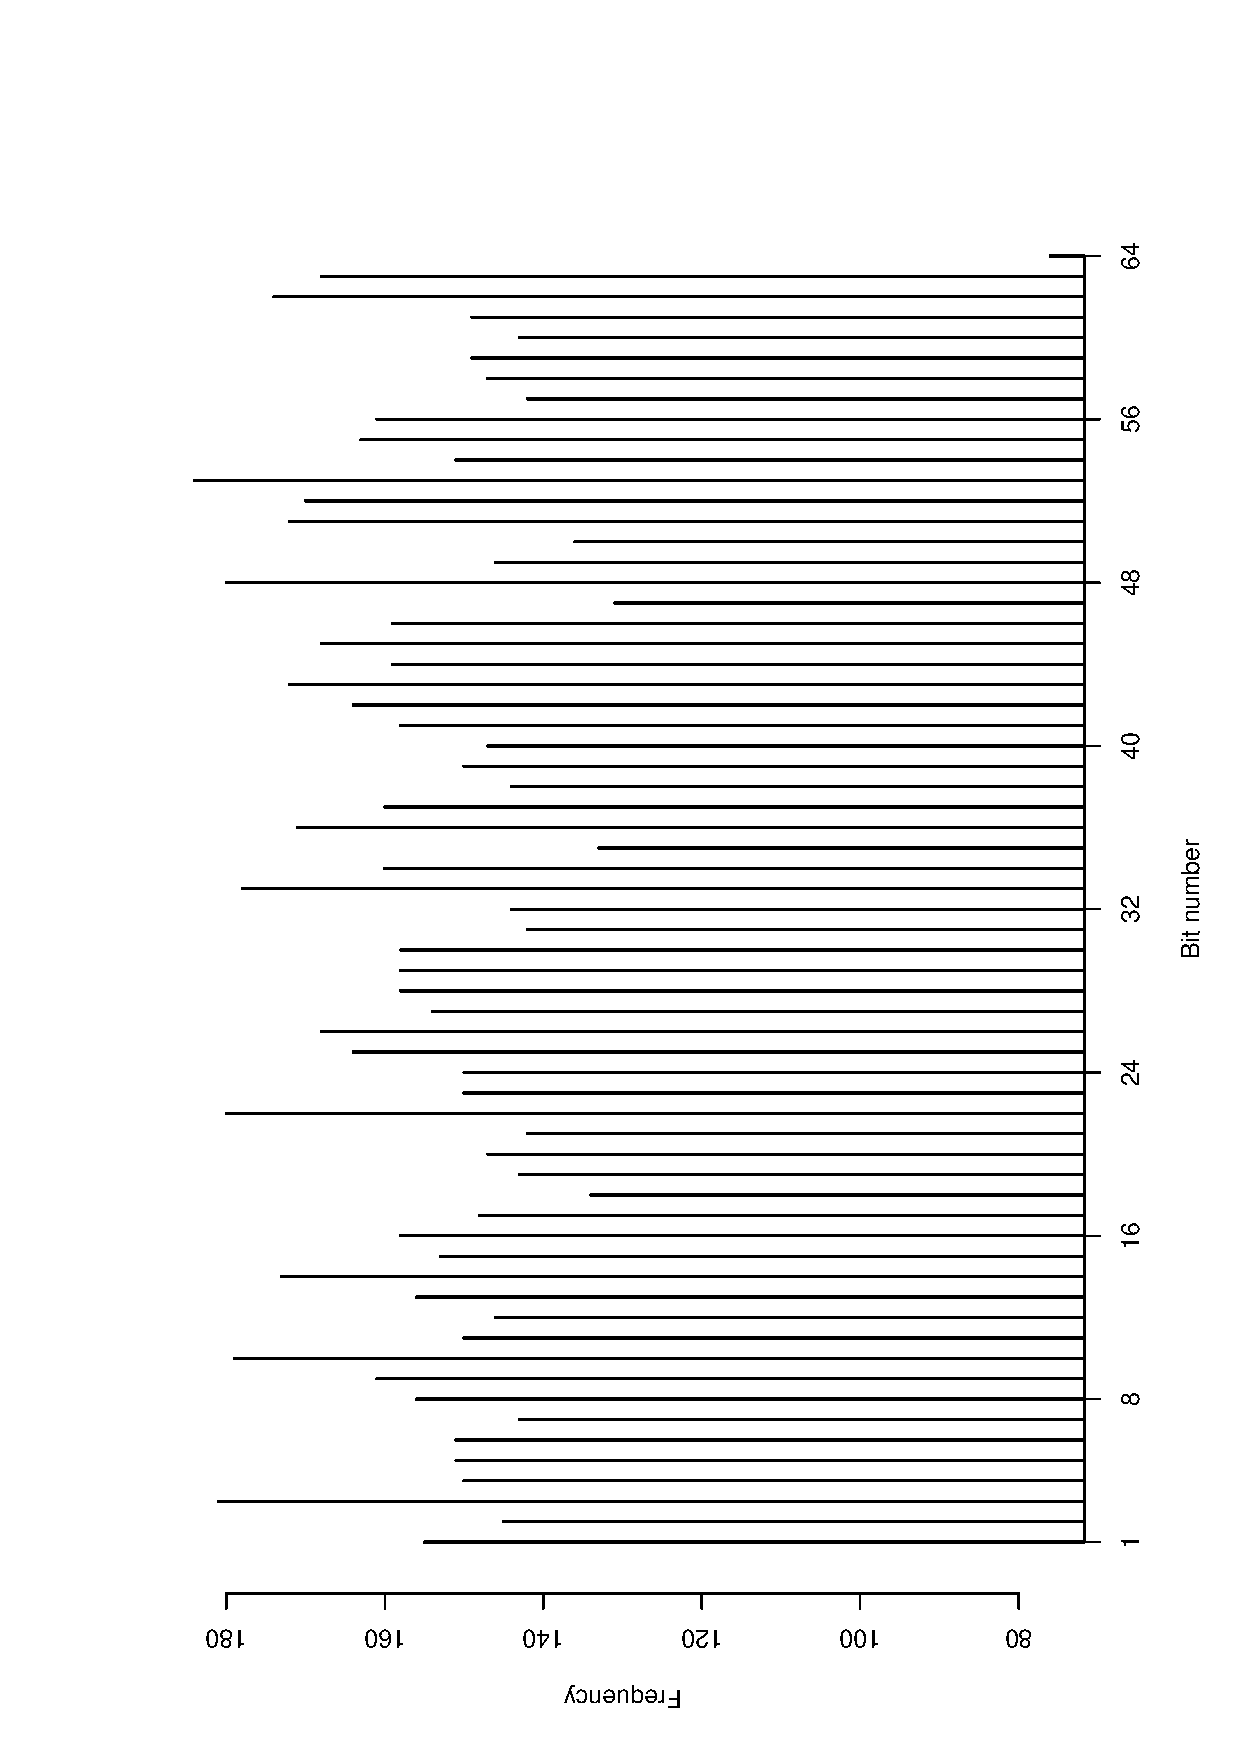
\includegraphics[scale=0.25,angle=-90,clip]{fig02}
  }
  \subfigure[$\alpha=1,\beta=32$]{
  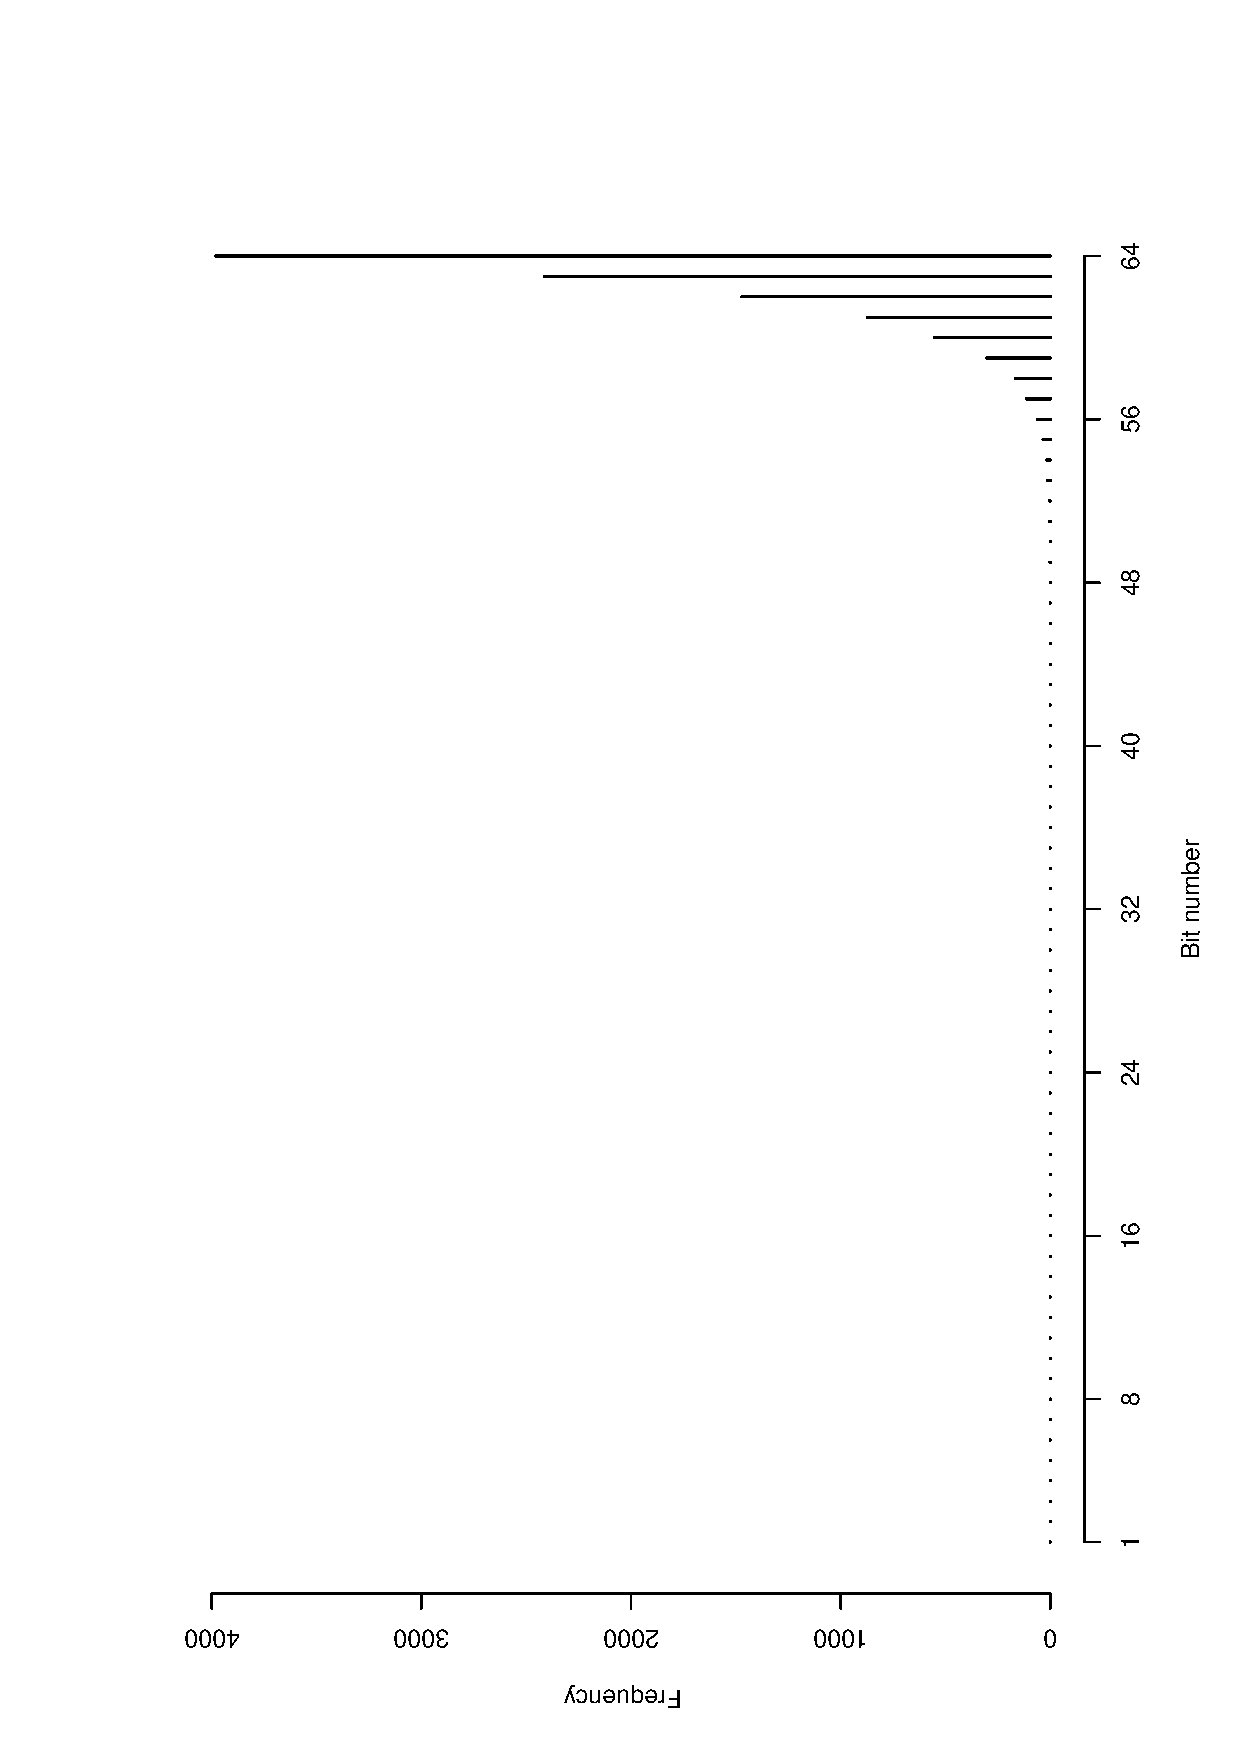
\includegraphics[scale=0.25,angle=-90,clip]{fig03}
  }
  \subfigure[$\alpha=32,\beta=1$]{
  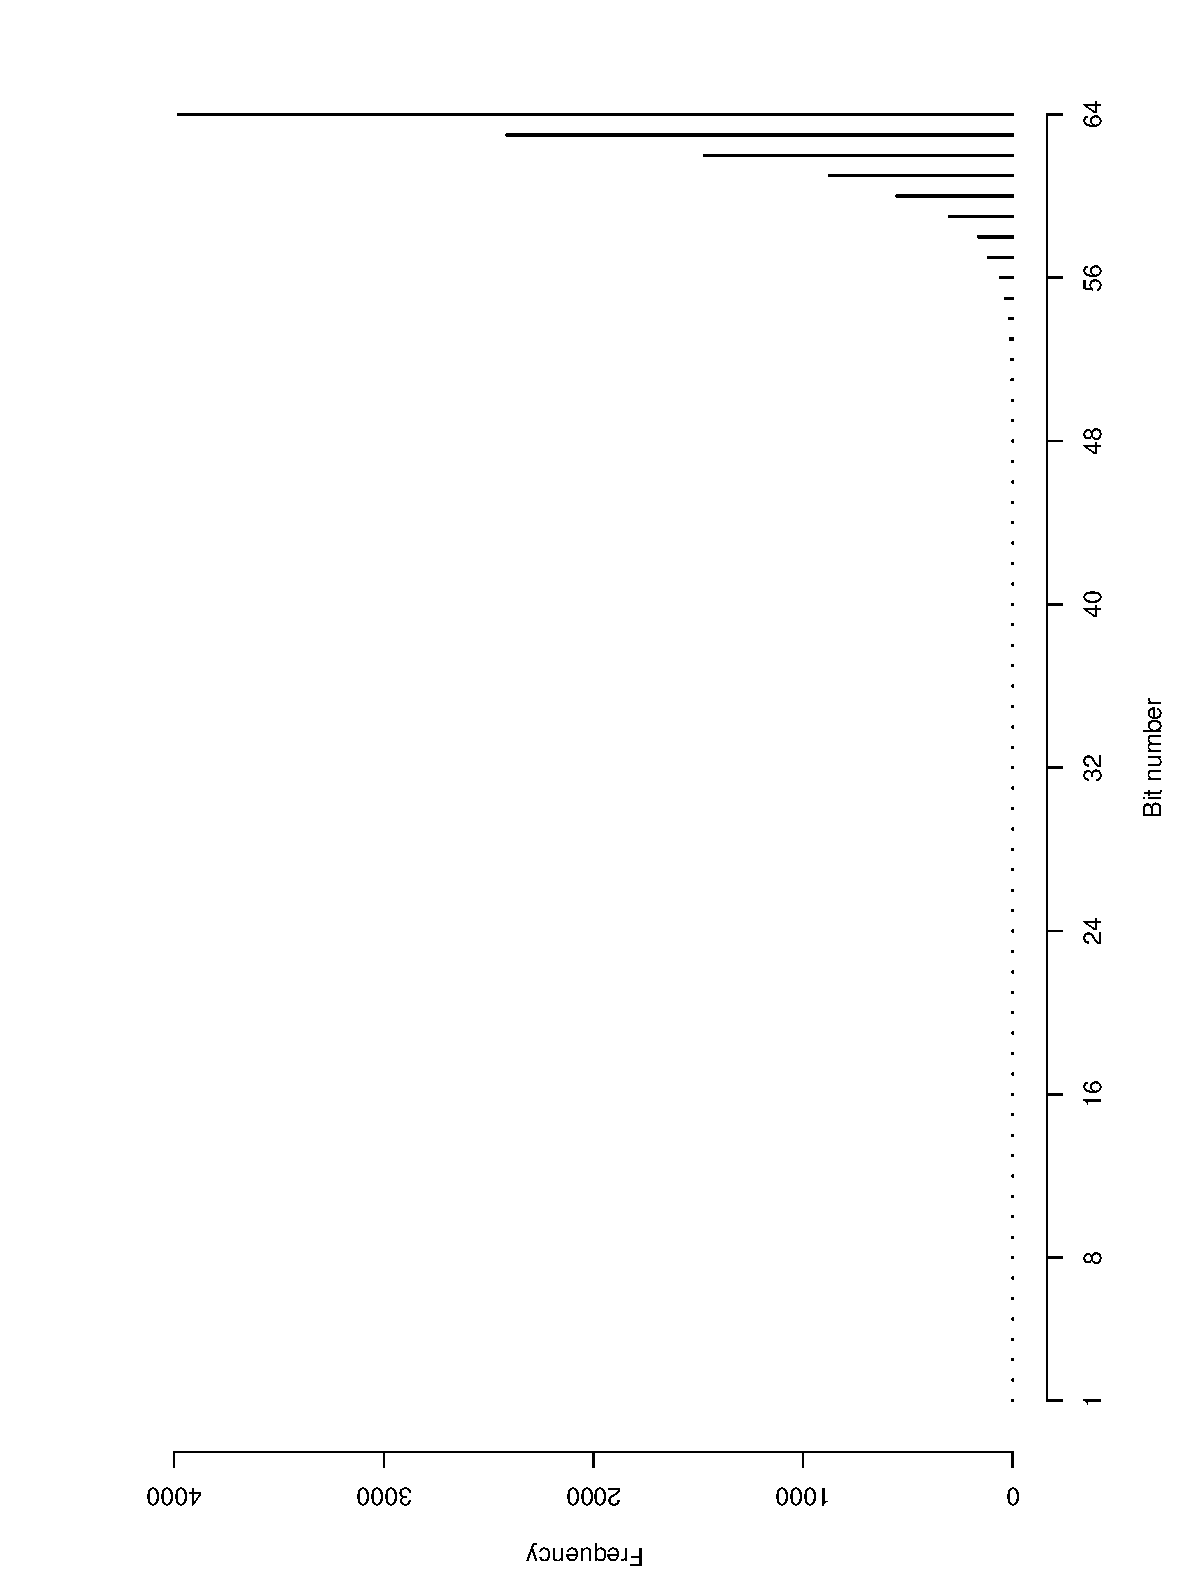
\includegraphics[scale=0.25,angle=-90,clip]{fig04}
  }
  \subfigure[$\alpha=64,\beta=64$]{
  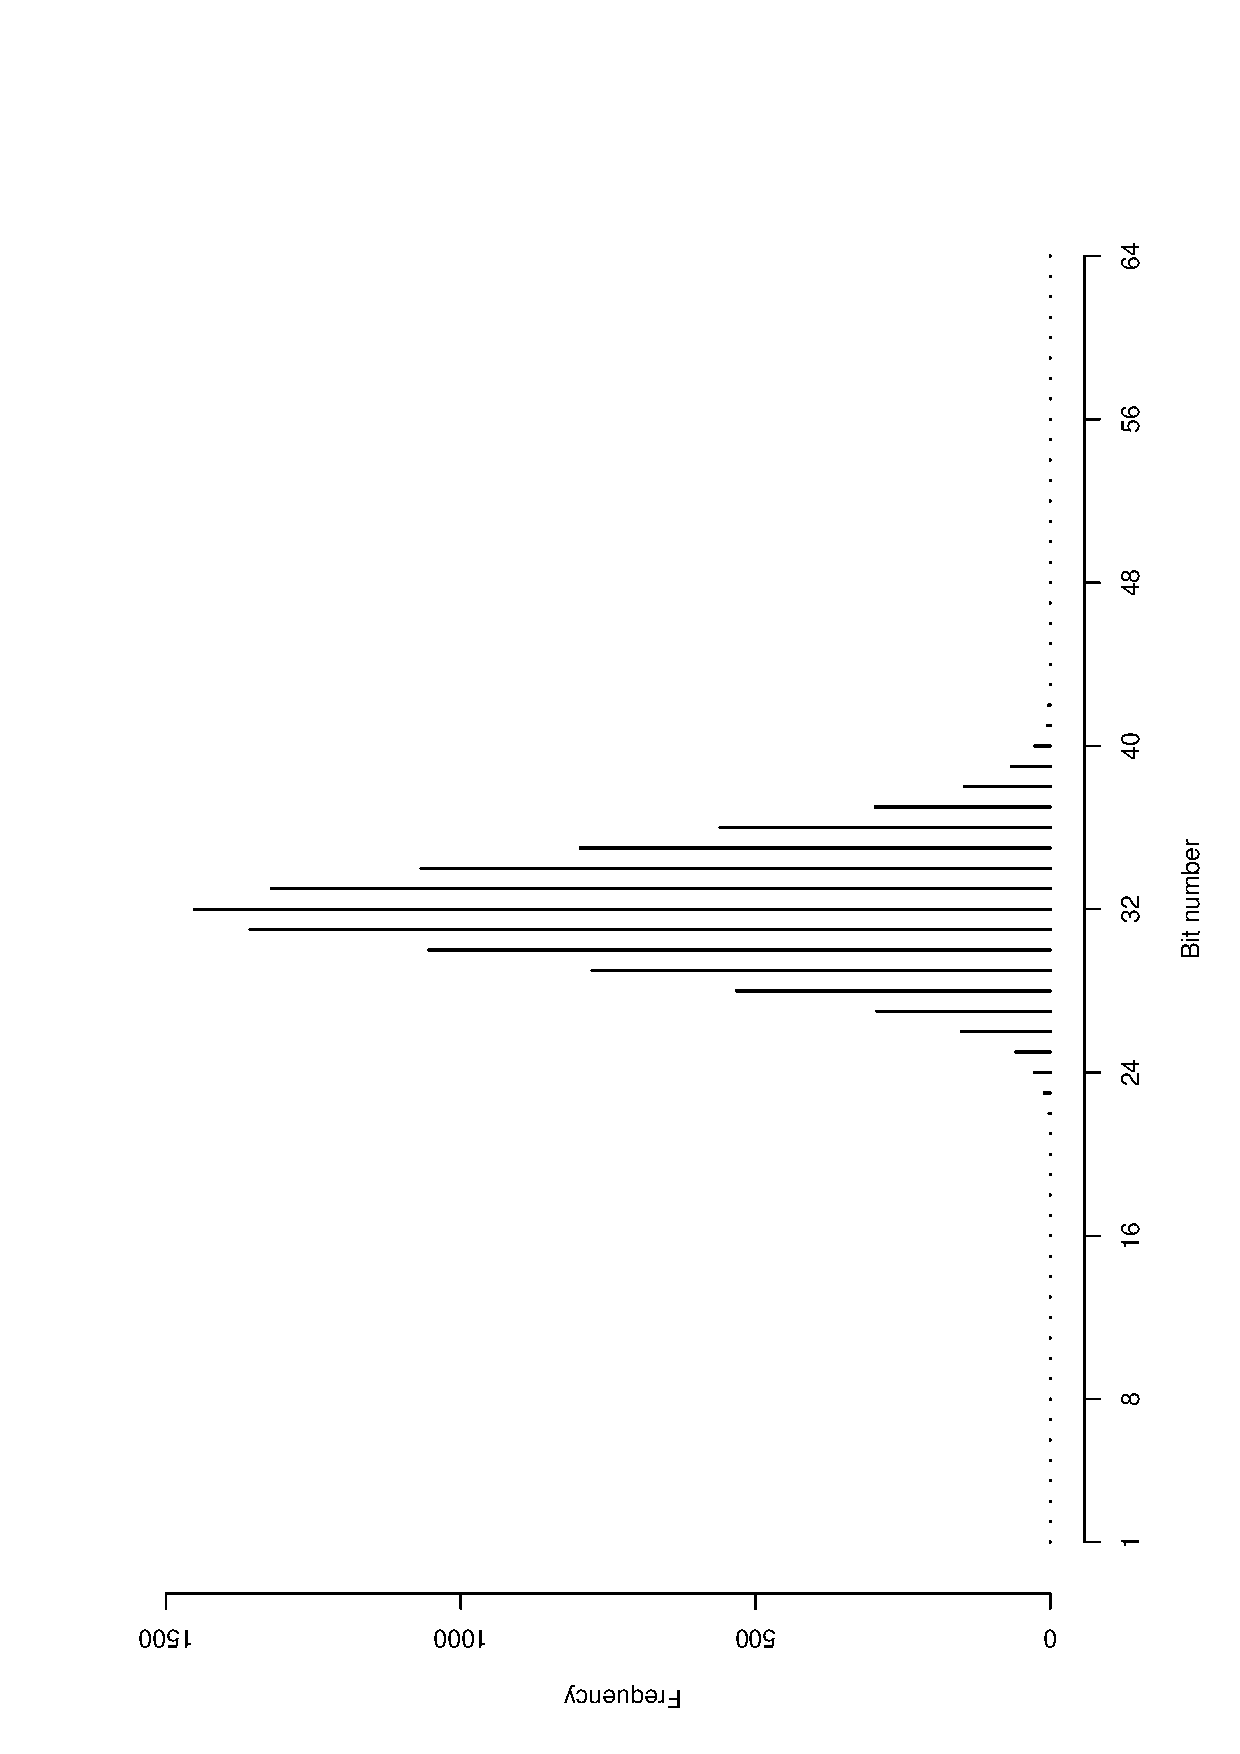
\includegraphics[scale=0.25,angle=-90]{fig05}
  }
  \caption{Histograms constructed from samples with 10,000 elements, generated from the Beta distribution. Below each histogram is possible to verify the parameters used.}
  \label{fig:02}
\end{figure}

As we intend to estimate the efficiency, the equations should be redefined in the sample function as can be seen in Equations \ref{eq:56} and \ref{eq:57}, methods 1 and 2, respectively, and $E(B)$ the expected value for the bit number (B) of number sample and $k$ largest expected value this sample.
 
\begin{equation}\label{eq:56}
 E(\zeta_1) = 1 - \frac{k}{64}
\end{equation}

\begin{equation}\label{eq:57}
 E(\zeta_2) = 1 - \frac{E(B)}{64} - \frac{k}{64}
\end{equation}
 
To define, based on a sample of the matrix M, which method should be used, we calculate the difference $R=E(\zeta_1)-E(\zeta_2)$. When $R>0$, the first method is more efficient than the method in the second data compression. At market $R<0$, the second method is more efficient. And otherwise, the two methods are the same.
 
In this first analysis, it is assumed that the values ​​of $\alpha$ and $\beta$ belong strictly to the interval $[1,64]$, the data are generated by modified Beta distribution $Beta(\alpha,\beta)$ and its representing the bit values required to represent elements of a matrix M. Generates three samples with size 10,000, it estimated efficiency values through the equations \ref{eq:56} and \ref{eq:57} and it calculated the difference $R$.

In Figure 3, you can verify the efficiency of the first (Figure (b)) and second (Figure (c)) methods, the relationship between them (Figure (a)) and the regions defined by the parameters alpha and beta, in which method is more efficient than the other (Figure (d)). In the Figures (b) and (c), it can observe that both methods are effective in the process of data compression, it reaching over 80 \% compression. Note that as the average (color scale) of the values ​​generated decreases, the compression rate increase, because the smaller the average value, the smaller bit number needed to represent these values. In the Figure (a) it is possible to verify the relationship between the methods defined by the difference $R$. Notice that most of the values ​​of the surface defined by R are negative, ie, the second method is more efficient than the first for most combinations. However, there is a small region, which can be seen in Figure (d), color white, indicating that for some values ​​generated from a modified 
beta distribution 
with parameters $\alpha$ and $\beta$, the first method is more efficient. This region in Figure (A) has red color and it indicates the average of data generated, then the bit number to represent a value in this region is larger and as a consequence first method makes more feasible.
 
\begin{figure}[h]
  \centering
%   \subfigure[$\alpha=1,\beta_1=1$]{
%   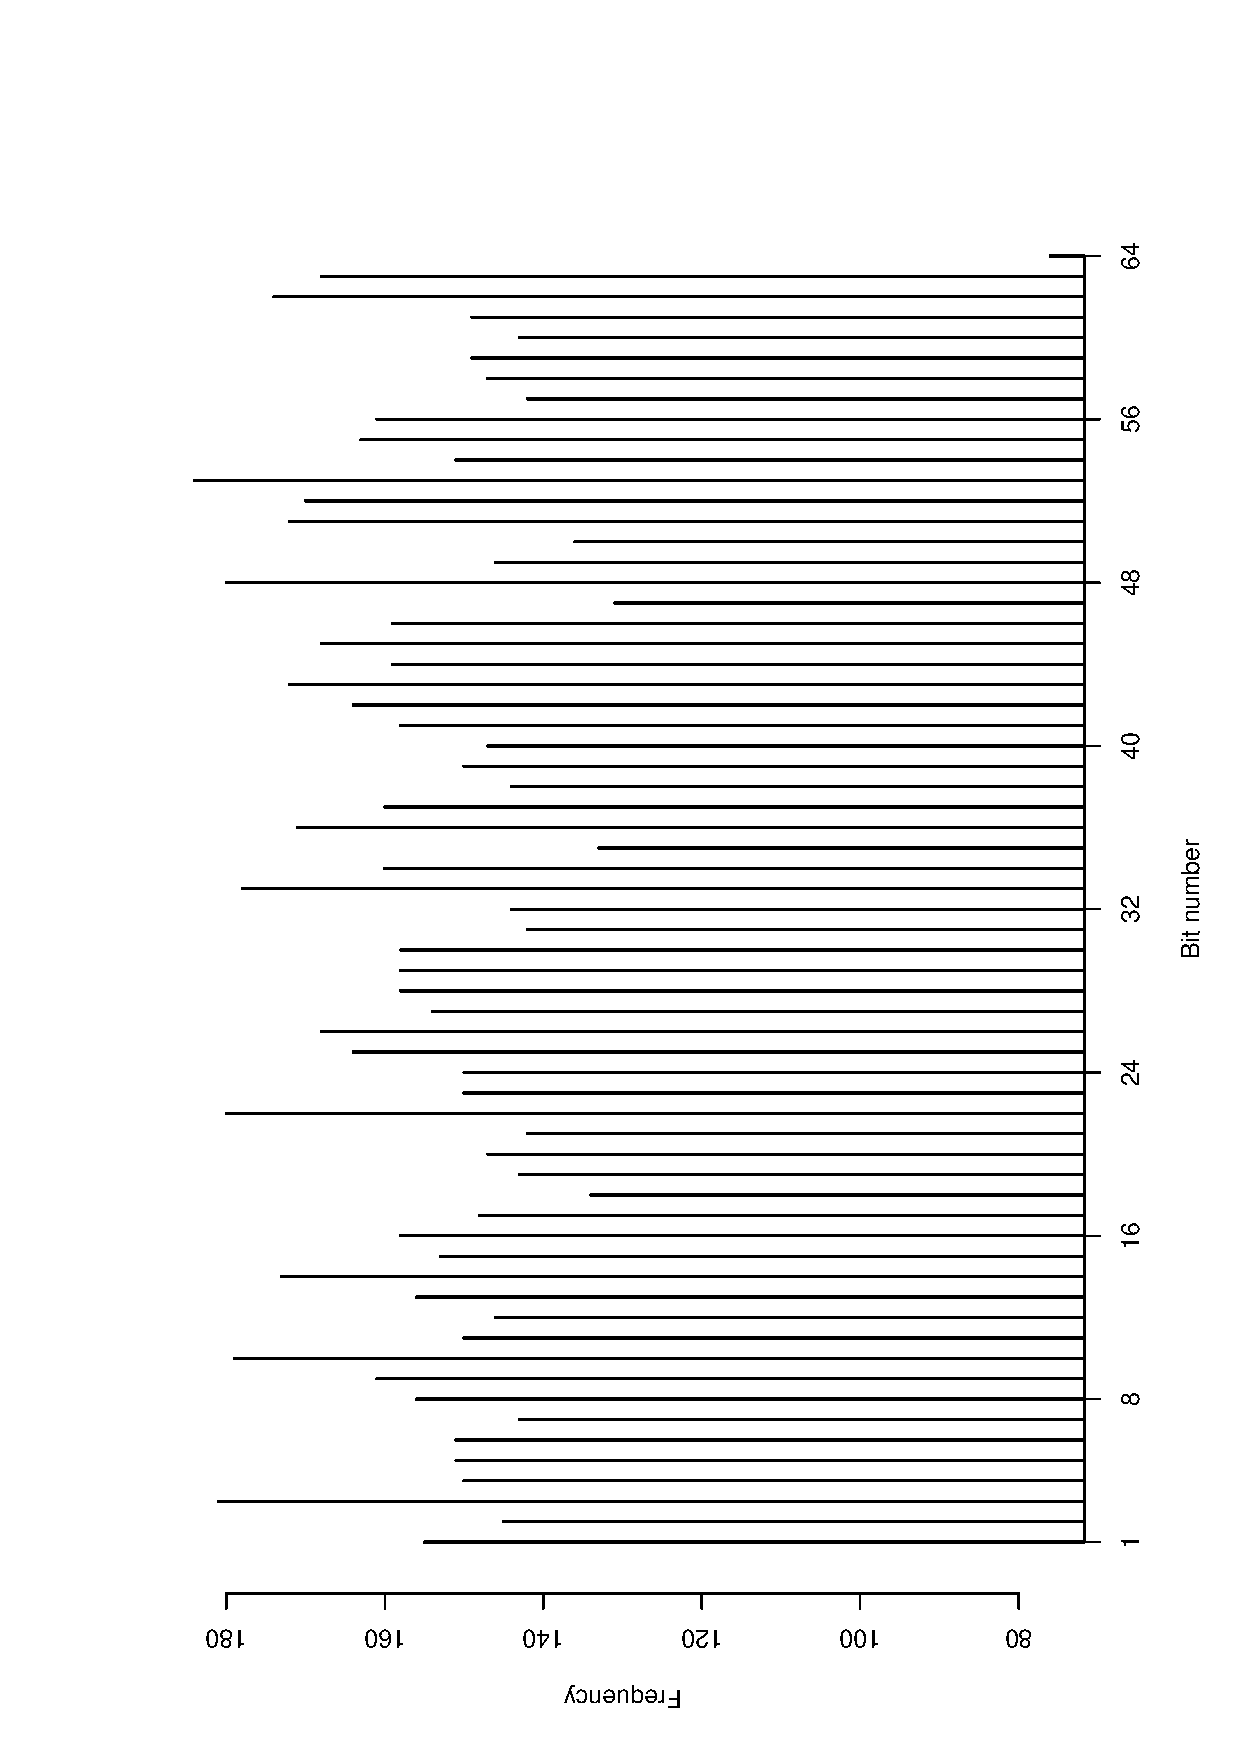
\includegraphics[scale=0.28,angle=-90,clip]{fig02}
%   }
%   \subfigure[$\alpha=1,\beta=32$]{
%   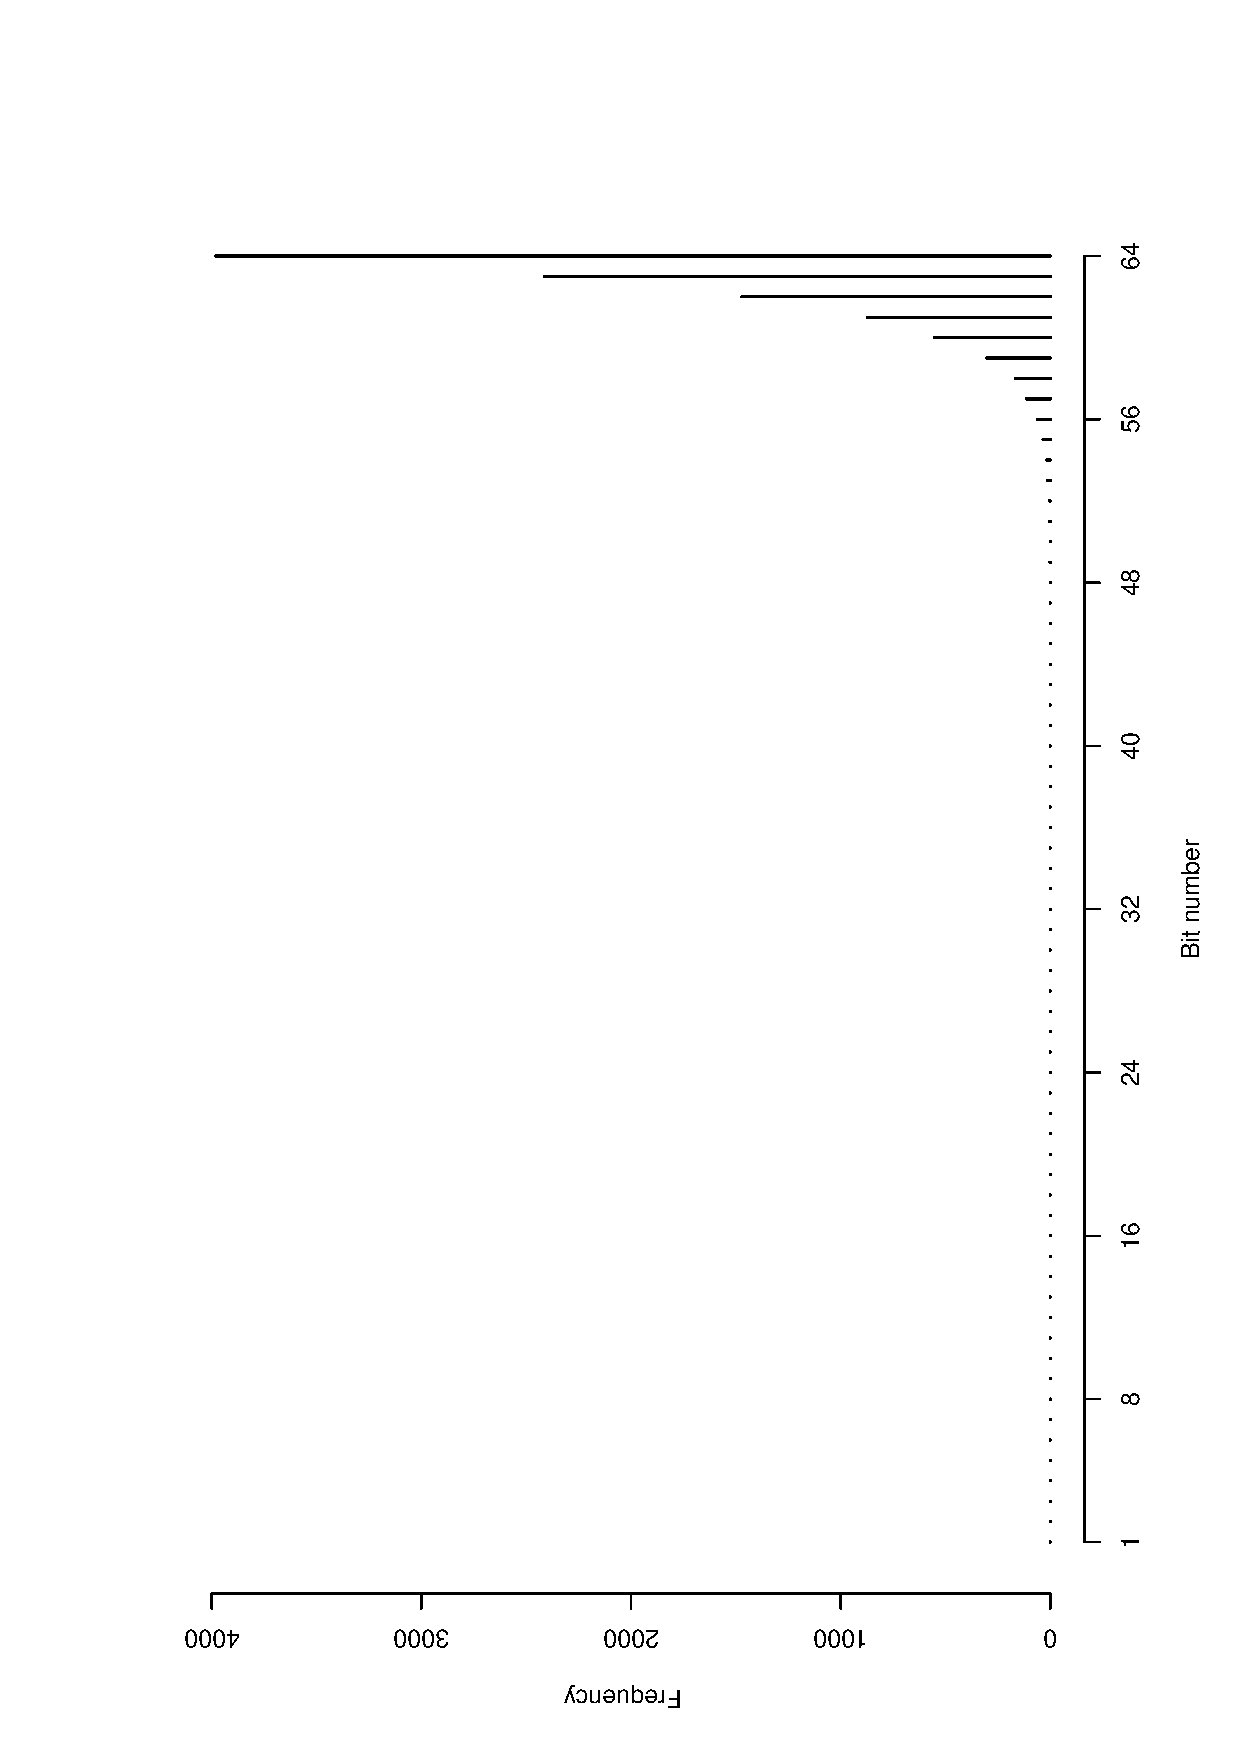
\includegraphics[scale=0.28,angle=-90,clip]{fig03}
%   }
%   \subfigure[$\alpha=32,\beta=1$]{
%   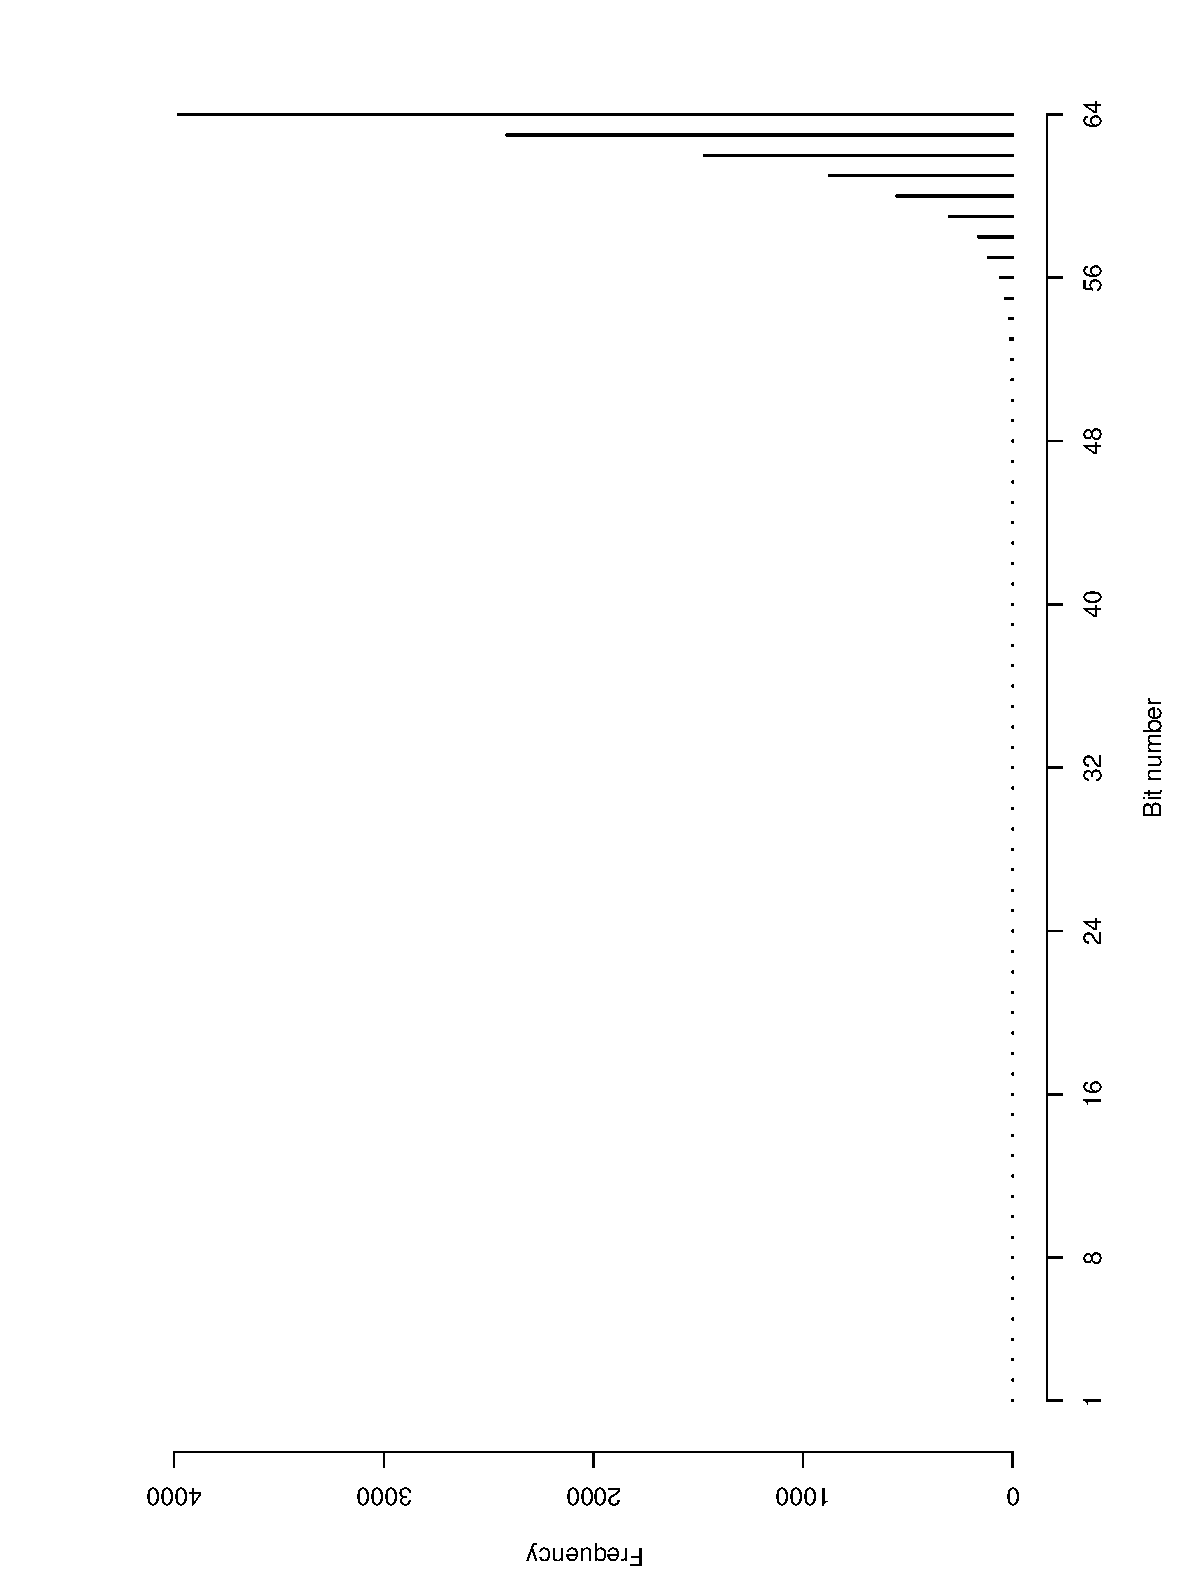
\includegraphics[scale=0.28,angle=-90,clip]{fig04}
%   }
%   \subfigure[$\alpha=64,\beta=64$]{
%   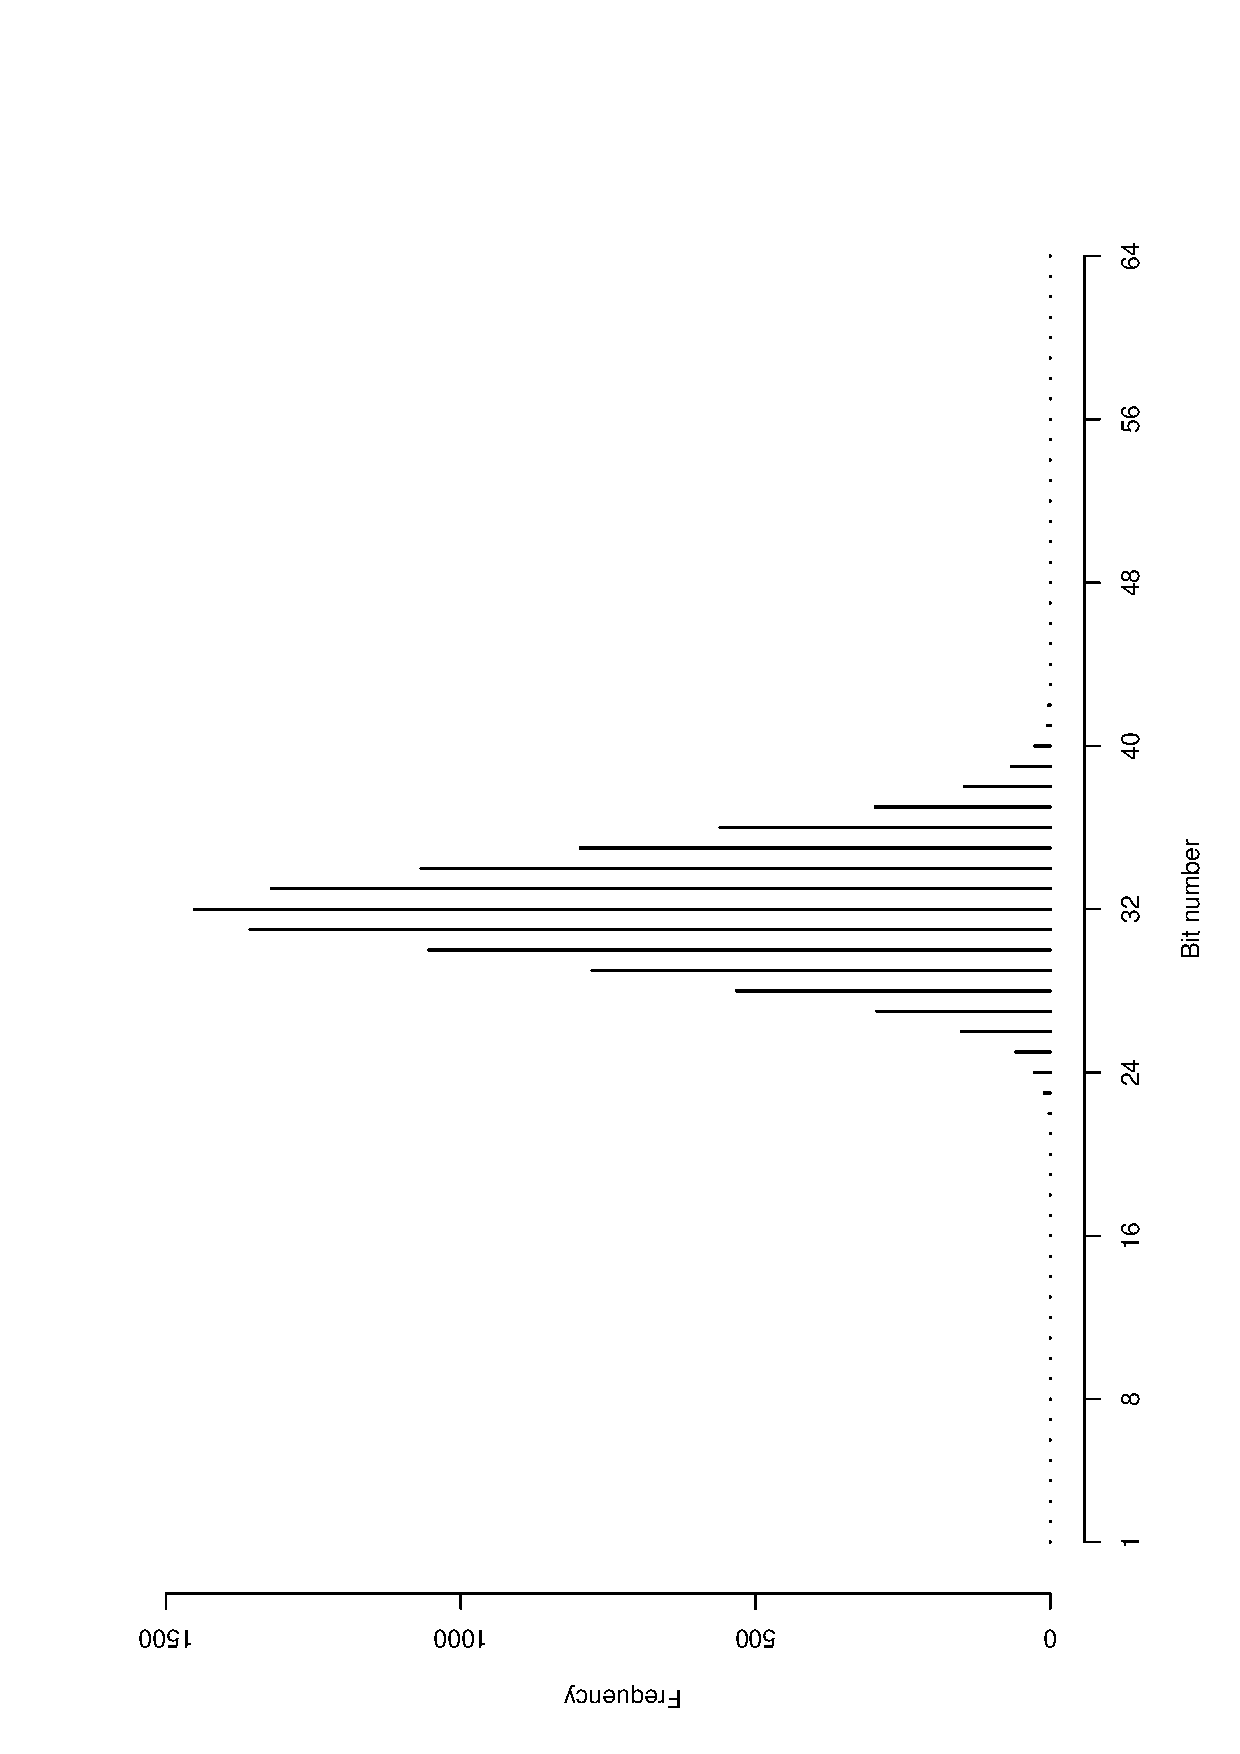
\includegraphics[scale=0.28,angle=-90]{fig05}
%   }
  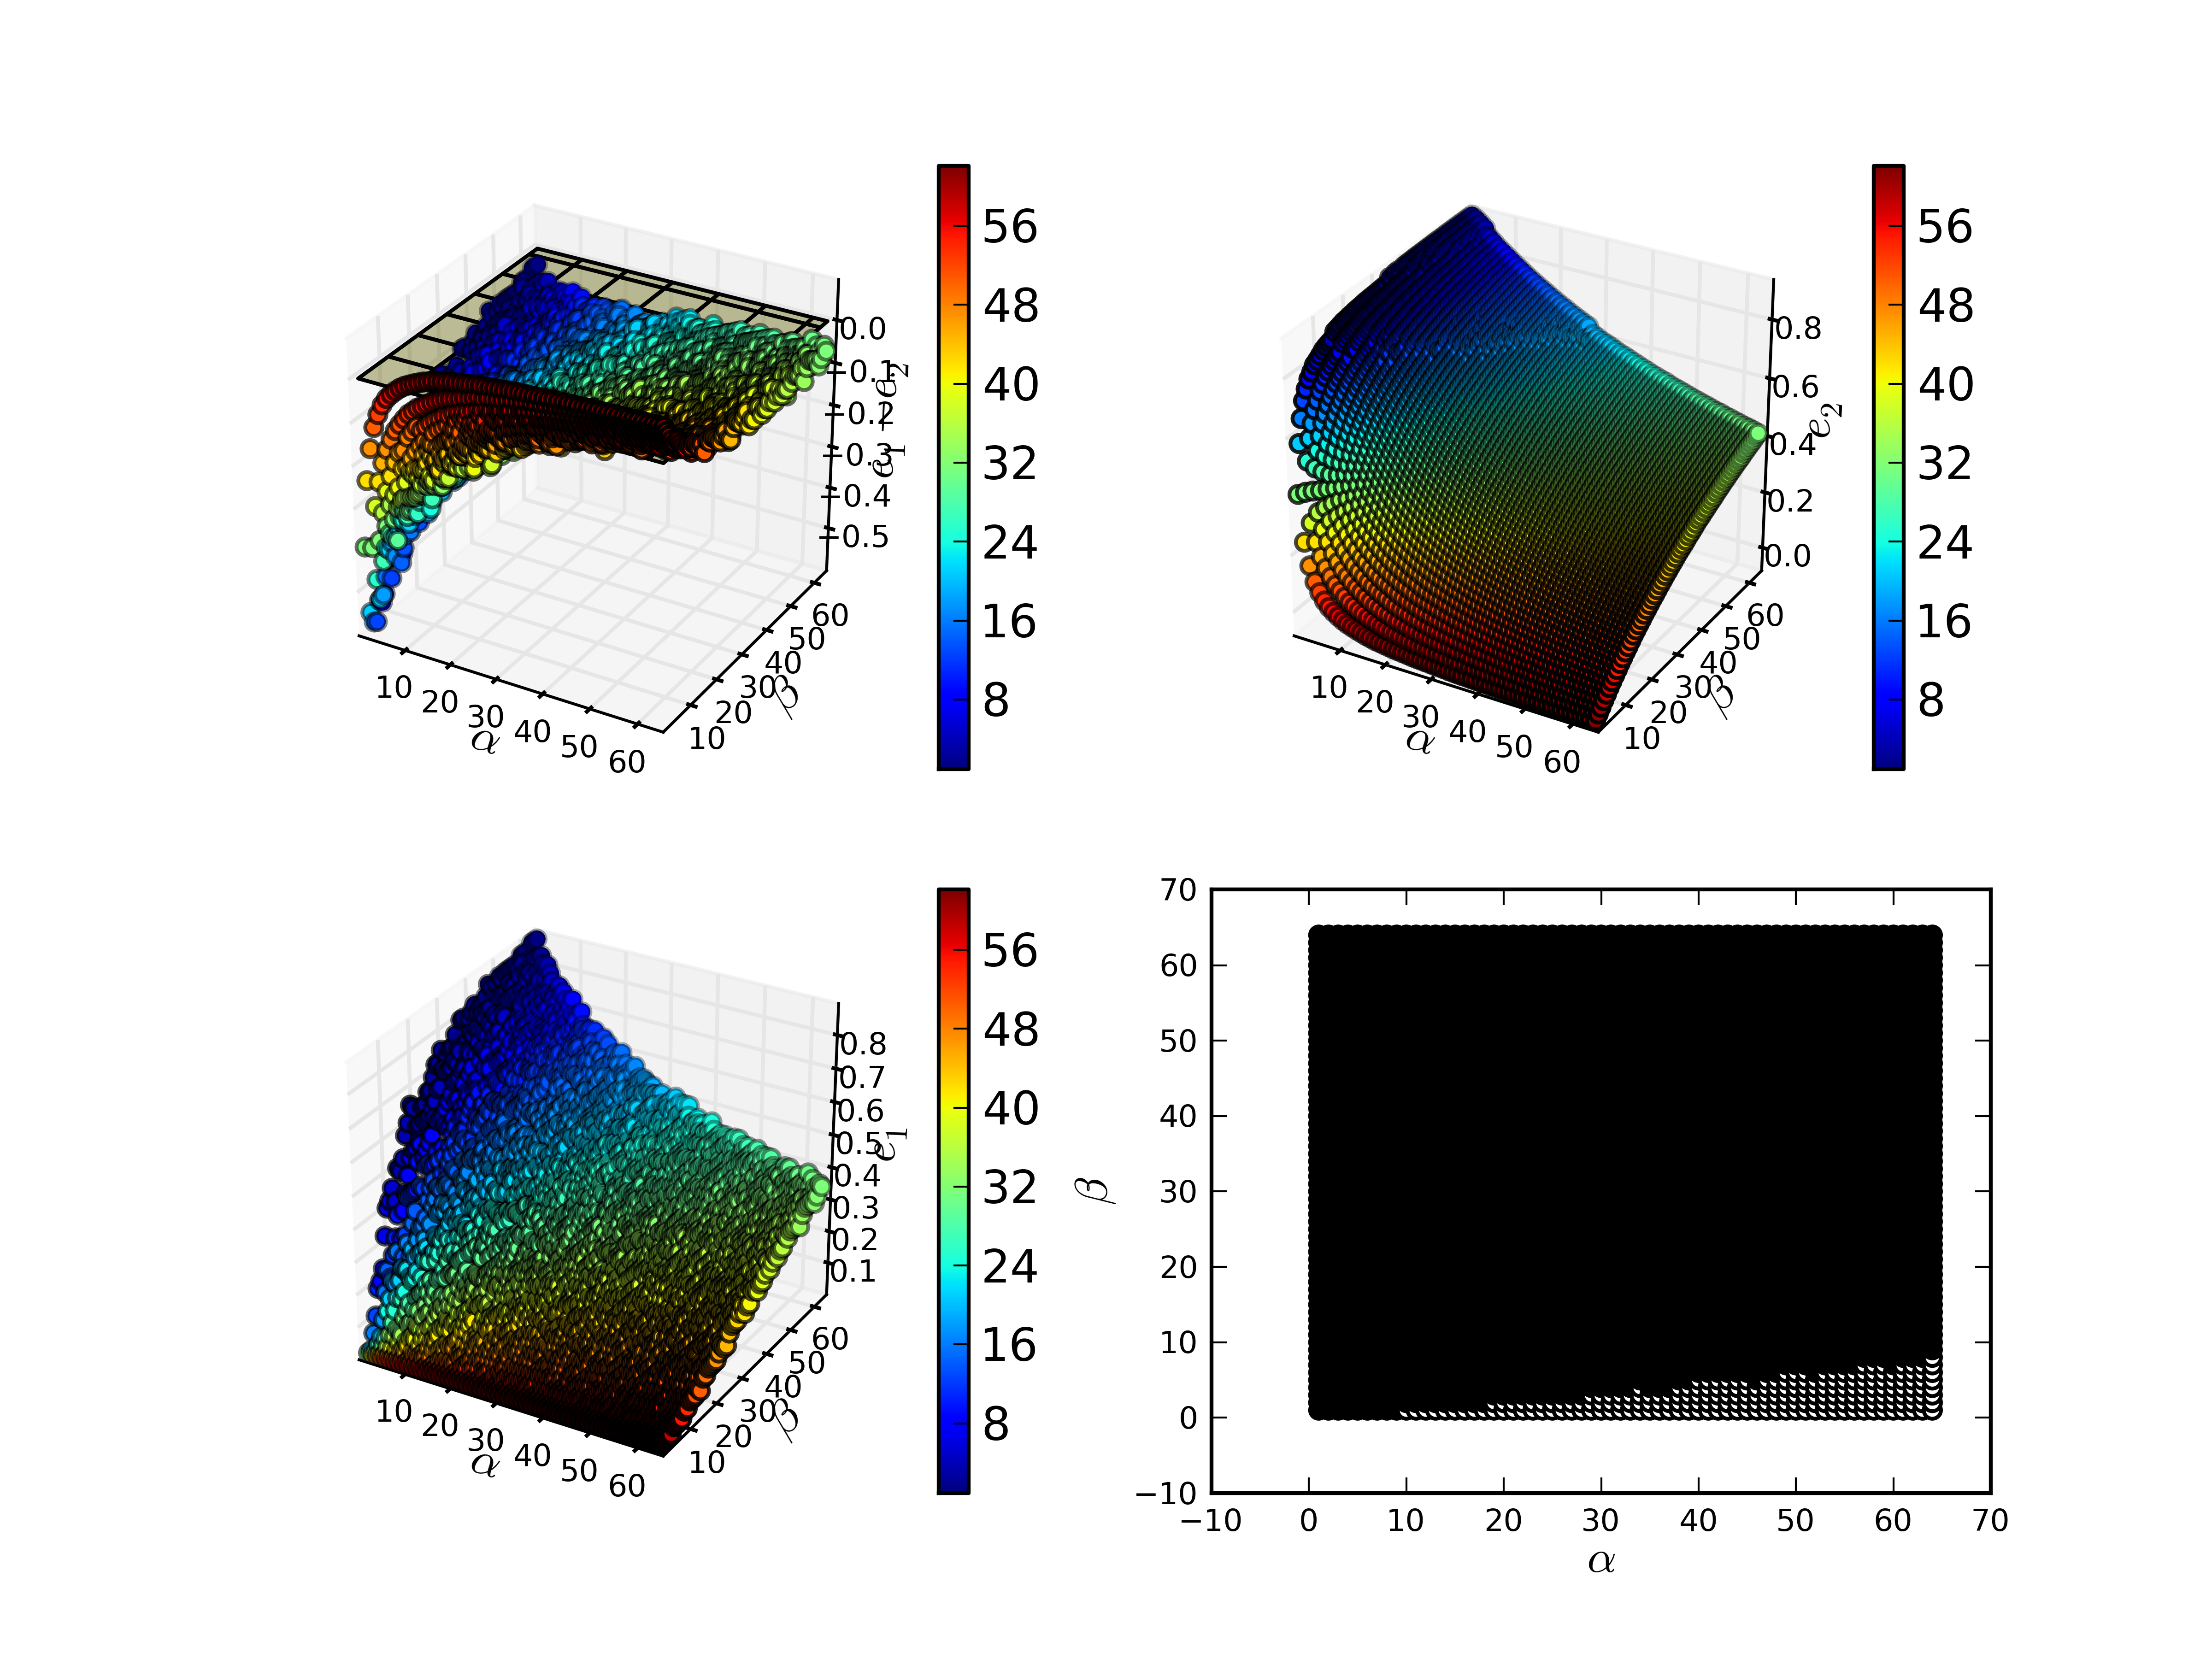
\includegraphics[scale=0.7]{simples.eps}
  \caption{Comparisons between methods I and II in relation to efficiency in the compression process. In the Figure (a) can see the difference between the efficiencies of each method $R$. It is verified that practically the entire surface has $R<0$, that is, the second method is more feasible for compressing the information generated from a Beta distribution modified $Beta(\alpha,\beta)$. However there is a region, which can be seen in Figure (d), color white, its indicates the values ​​generated from values ​​determined by $\alpha$ and $\beta$, the first method is more efficient. This region can be identified in Figure (a) in red, indicating that the generated values ​​have larger average ​​and require more bits to be represented. This demand makes the first method more feasible for the values ​​generated in this configuration. In Figures (b) and (c), it can be seen that both methods are effective with respect to high data compression rates generated from a Beta distribution $Beta(\alpha,\beta)$. Note, in 
both figures, the value of the efficiency of the compression increases with reduction of the average number of generated. This is due to reducing the bit number required to represent those values.}
  \label{fig:03}
\end{figure}
 
Another analysis can be performed from the combination of two variables, $B_1$ and $B_2$, following a Beta distribution with parameters $Beta(\alpha_1$,$\beta_1)$ and $Beta(\alpha_2$,$\beta_2)$, respectively, it can calculate the bit number (B) to the mixture of these two distributions. To simplify operations, it is considered that $\lambda = 0.5$, ie, the mixture will have half the numbers generated from the distribution $Beta(\alpha_1,\beta_1)$ and the other part distribution $Beta(\alpha_1,\beta_1)$. The expected value for this mixture is shown in Equation \ref{eq:58}.
 
\begin{equation}\label{eq:58}
 E(B) = 0.5 E(B_1) + 0.5 E(B_2)
\end{equation}
 
Now, we must redefine the functions for calculating the efficiency. Some modifications should be considered, the first being related to Equation \ref{eq:56} which represents the expected value for efficiency using the first method. Thus, the function is defined only in terms of $B$, since for this method, the important is only the bit greater number than a demand matrix element M (Equation \ref{eq:59}). As for the second method​​, emphasizing that the constant $k$, is a function of $B$, again because they are the highest values ​​for represent an element of M (Equation \ref{eq:60}).

\begin{equation}\label{eq:59}
 E(\zeta_1) = 1 - \frac{k(E(B))}{64}
\end{equation}

\begin{equation}\label{eq:60}
 E(\zeta_2) = 1 - 0.5\frac{E(B_1)}{64} - 0.5\frac{E(B_2)}{64} - \frac{k(E(B))}{64}
\end{equation}
 
How the values ​​of the alphas and betas strictly belong to the interval $[1,64]$, ie, representing the values ​​of bits required to represent elements of a matrix M, generating a sample with size $n=10,000$ and estimated efficiency values through the equations \ref{eq:59} and \ref{eq:60}, and soon after, we calculate the efficiency difference $R$ of values ​​calculated. 

Before you can calculate the difference of efficiencies, we will analyze some data histograms, constructed from samples with 10,000 elements, generated from beta mixtures distributions. For this, we consider that the values ​​of $\alpha_1$, $\beta_1$, $\alpha_2$ and $\beta_2$ described in Figures \ref{fig:02A} and \ref{fig:02B}. One can see that with different values ​​for the alphas and betas, it becomes possible to construct different histograms. Each histogram of this regards the bit distribution needed to fill a matrix. For each of the samples generated from alphas and betas, their efficiency is calculated methods I and II. The comparison between the methods can be seen in Table \ref{tab:06}. The results indicate that over 90 \% of the samples with method II was more efficient in the data compression process. This result indicates that for matrices, in which mixtures can be associated probability distributions method II is the most indicated. Analyzing the efficiencies histogram, Figure \ref{fig:1415} is 
verified that the method II (Figure \ref{fig:15)}, on average, presents greater efficiency values ​​in the data compression process of the method I (Figure \ref{fig:14}). Again confirming the results presented. Analyzing Figure \ref{fig:1617}, it can be seen that the regions but which the mean values ​​of mixed distributions, represented by $\mu_1$ and $\mu_2$, indicate that for high values​​, the method I is more appropriate (Figure \ref{fig:16}), provided that the variability of the data is small (Fig. \ref{fig:17}).

\begin{figure}[h]
  \centering
  \subfigure[$\alpha_1=1,\beta_1=1,\alpha_2=1,\beta_2=1$]{
  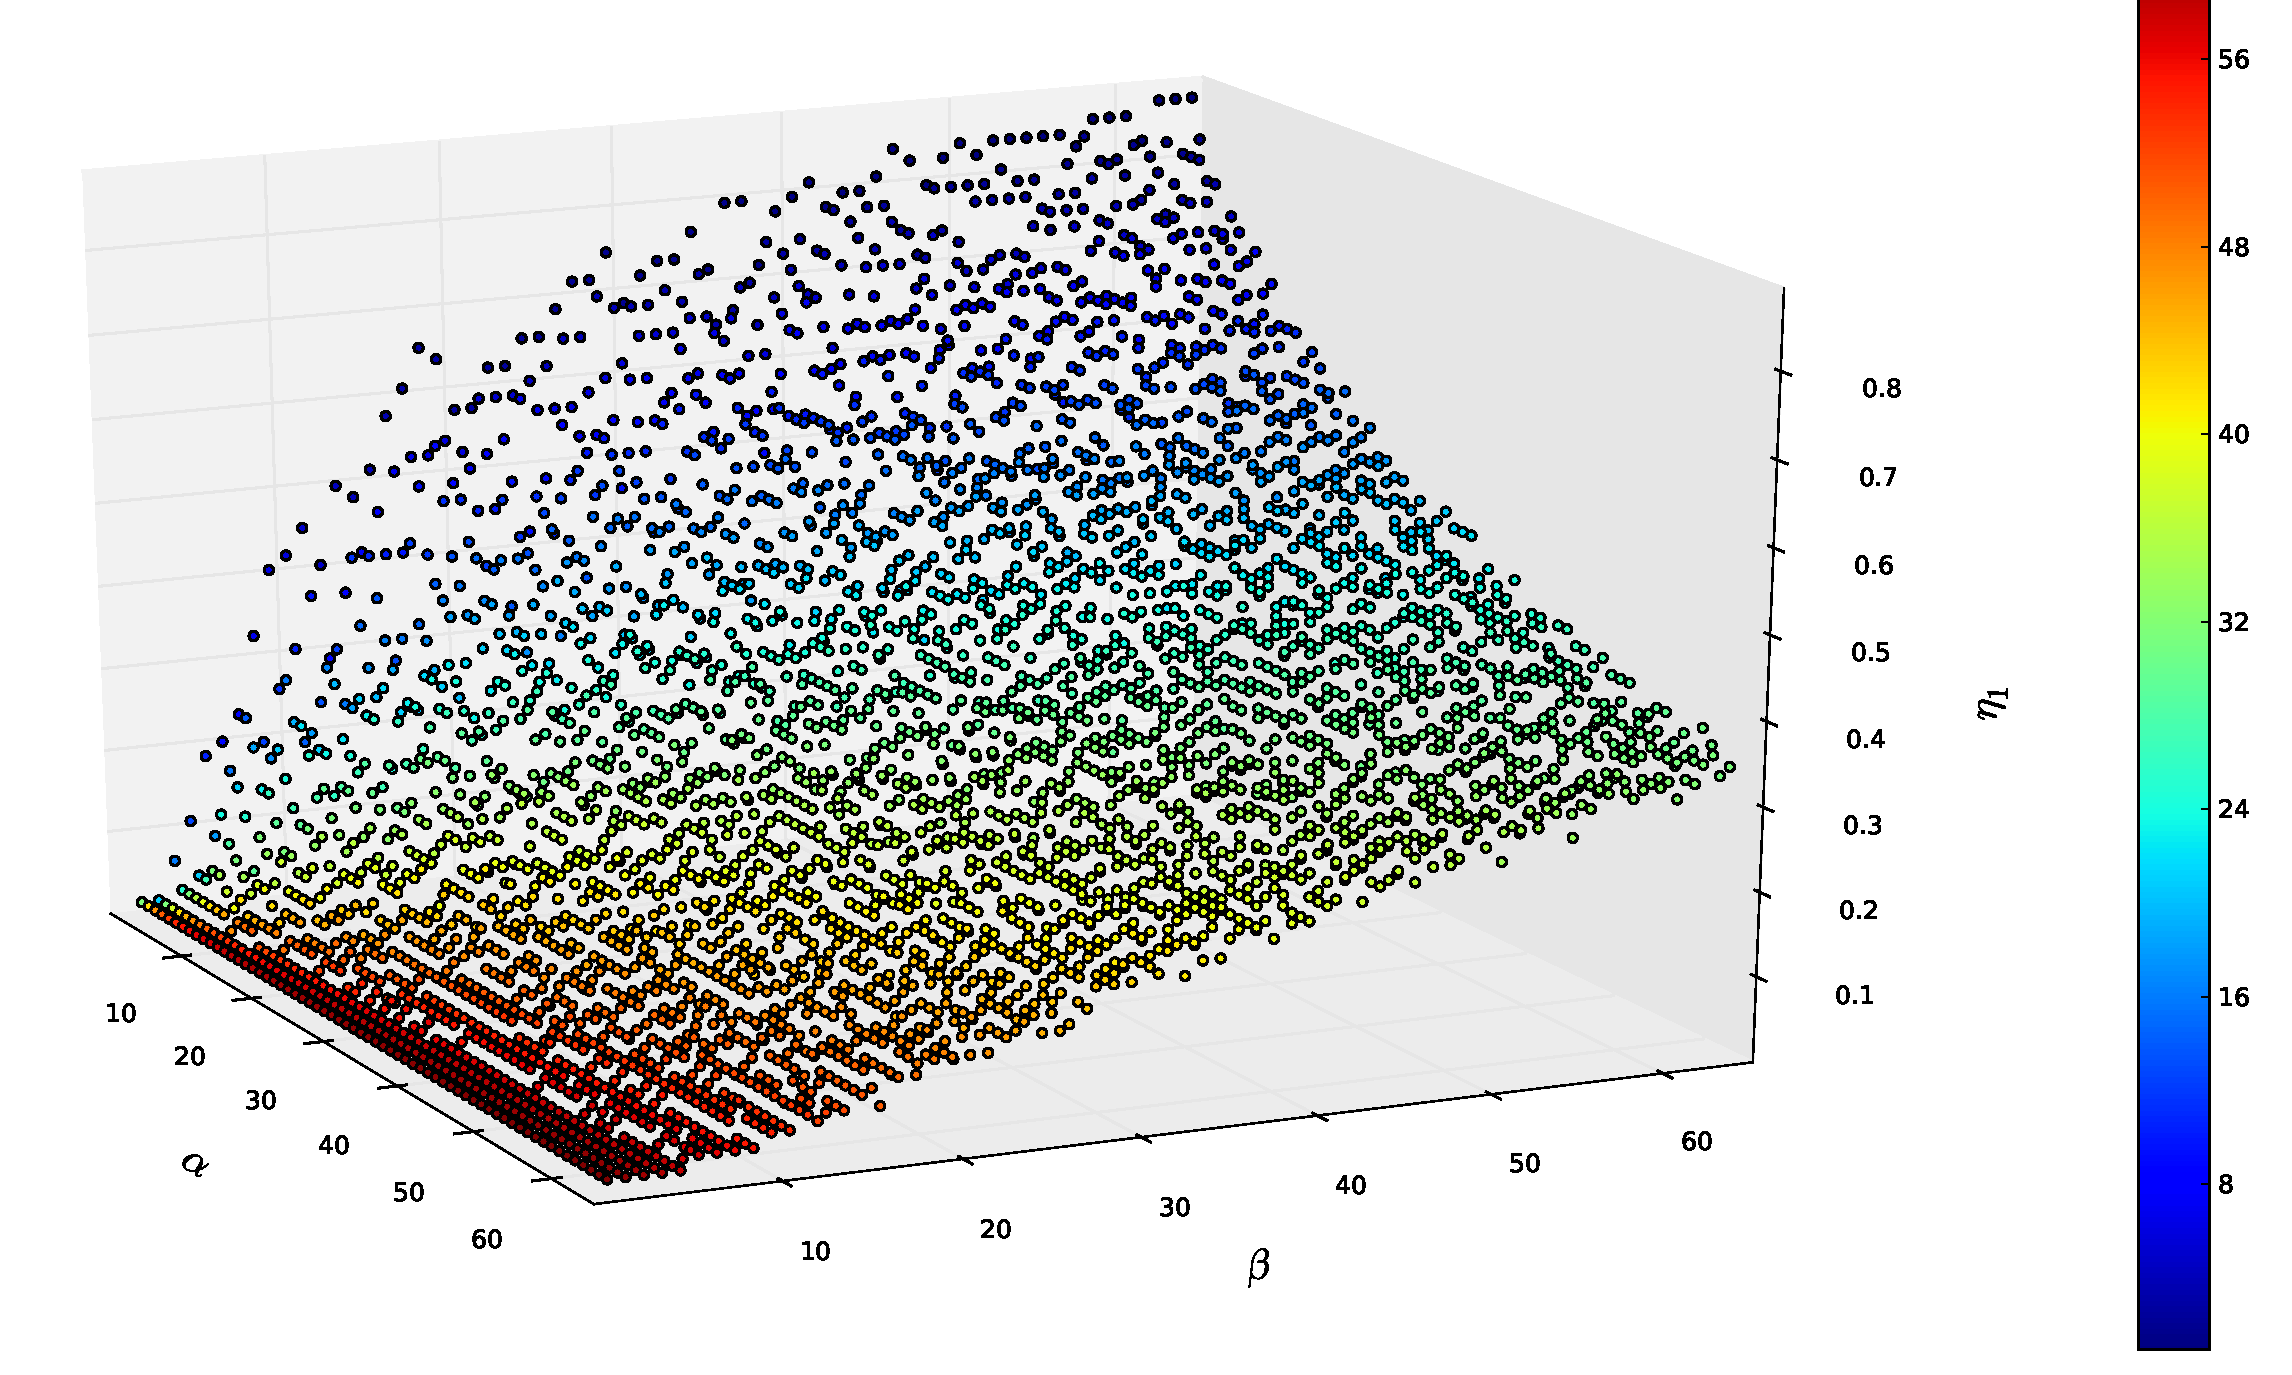
\includegraphics[scale=0.28,angle=-90,clip]{fig06}
  }
  \subfigure[$\alpha_1=1,\beta_1=32,\alpha_2=32,\beta_2=1$]{
  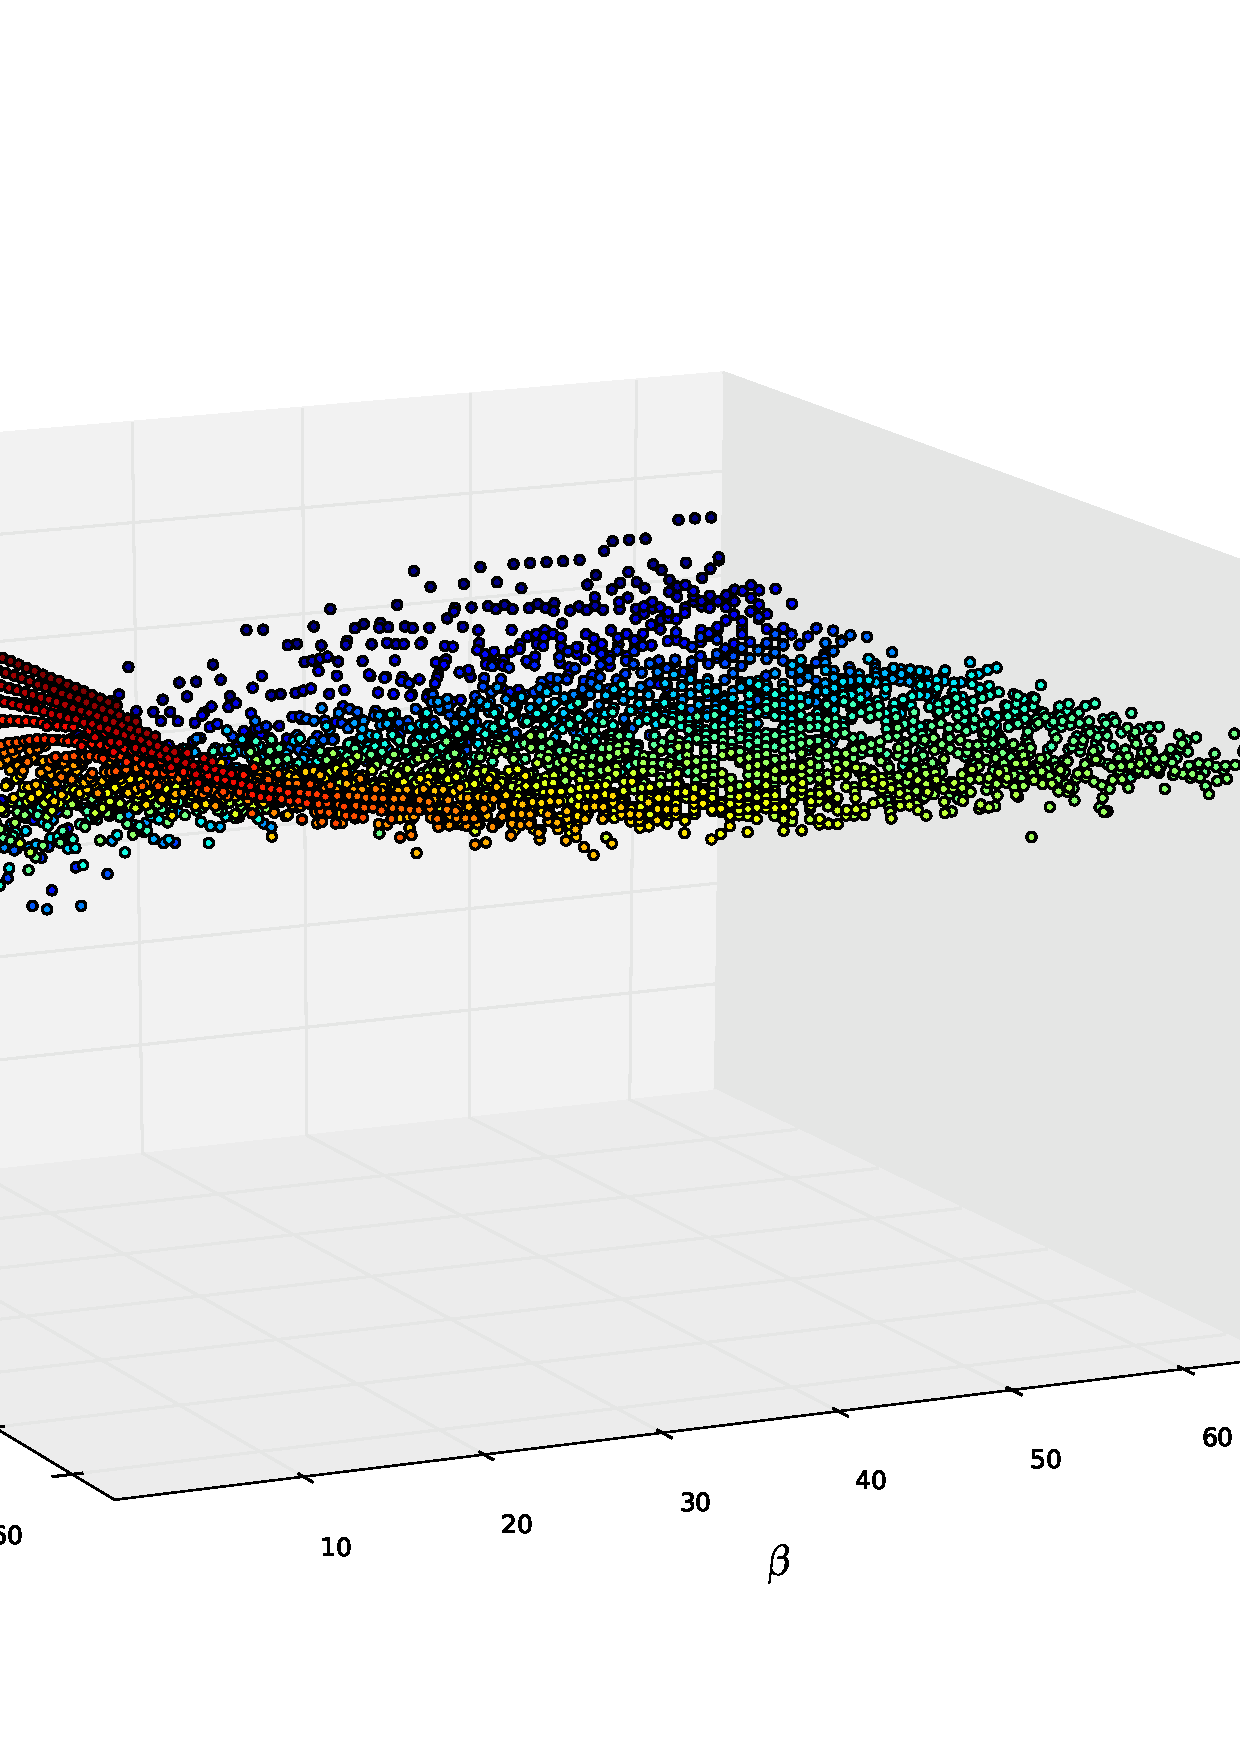
\includegraphics[scale=0.28,angle=-90,clip]{fig07}
  }
  \subfigure[$\alpha_1=32,\beta_1=32,\alpha_2=32,\beta_2=32$]{
  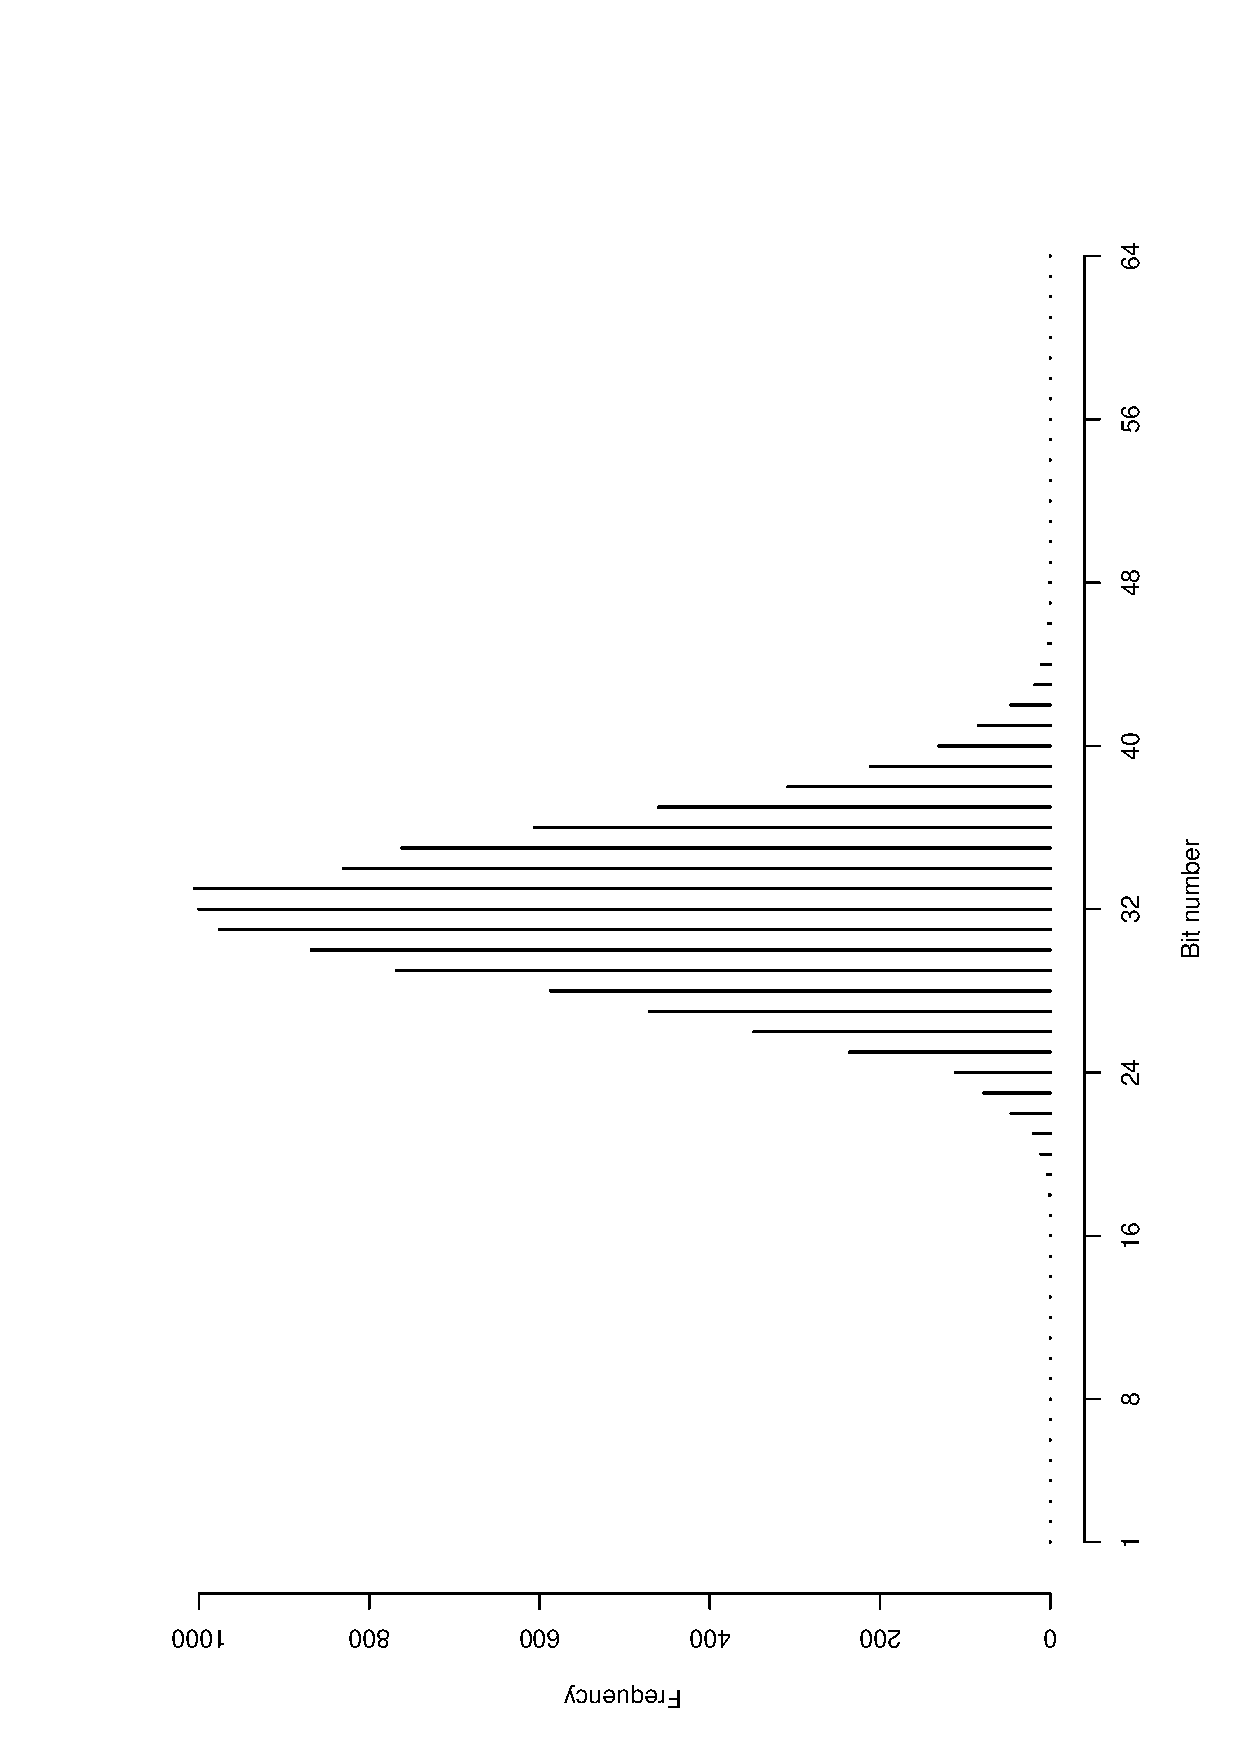
\includegraphics[scale=0.28,angle=-90,clip]{fig08}
  }
  \subfigure[$\alpha_1=64,\beta_1=32,\alpha_2=32,\beta_2=64$]{
  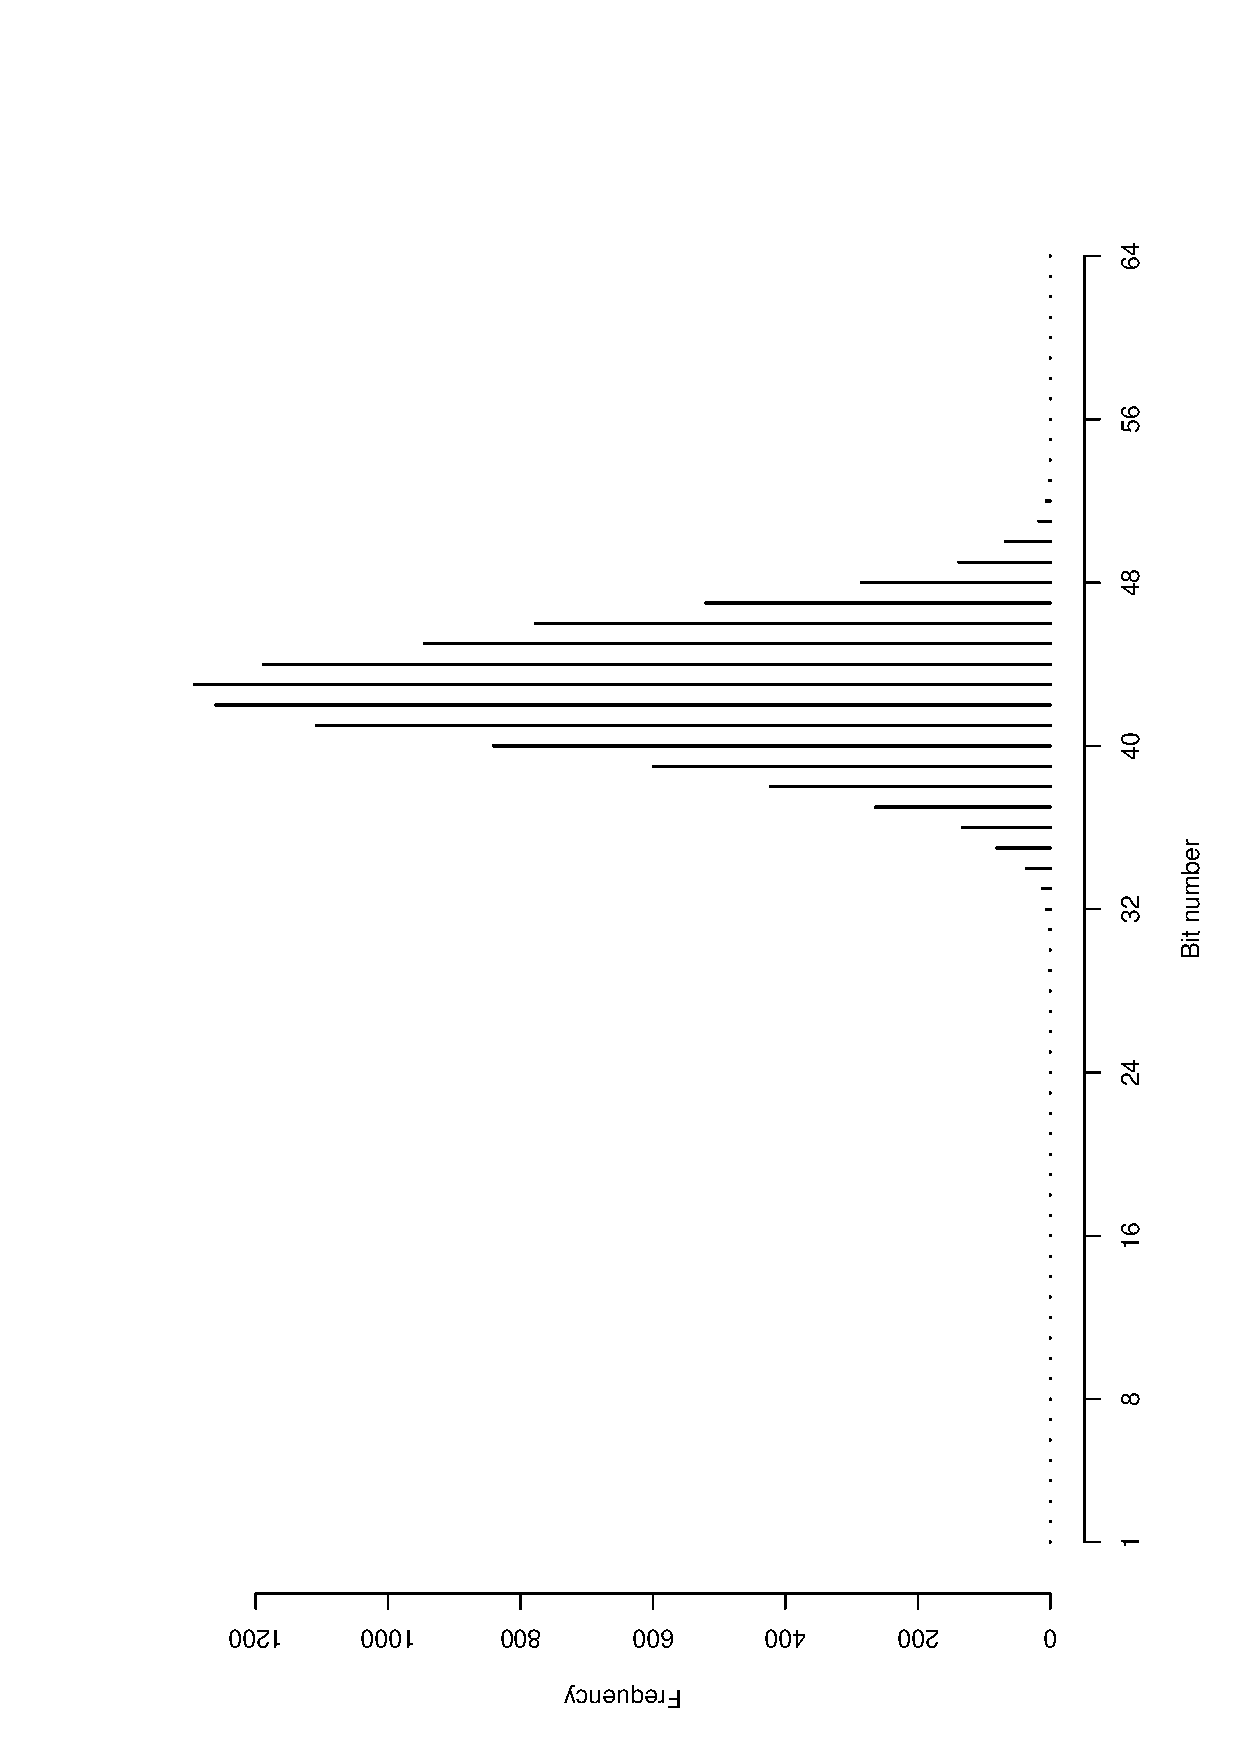
\includegraphics[scale=0.28,angle=-90]{fig09}
  }
  \caption{Histograms constructed from samples with 10,000 elements, generated from the combination of two distributions Betas. Below each histogram is possible to verify the parameters used..}
  \label{fig:02A}
\end{figure}

\begin{figure}[h]
  \centering
  \subfigure[$\alpha_1=64,\beta_1=48,\alpha_2=1,\beta_2=48$]{
  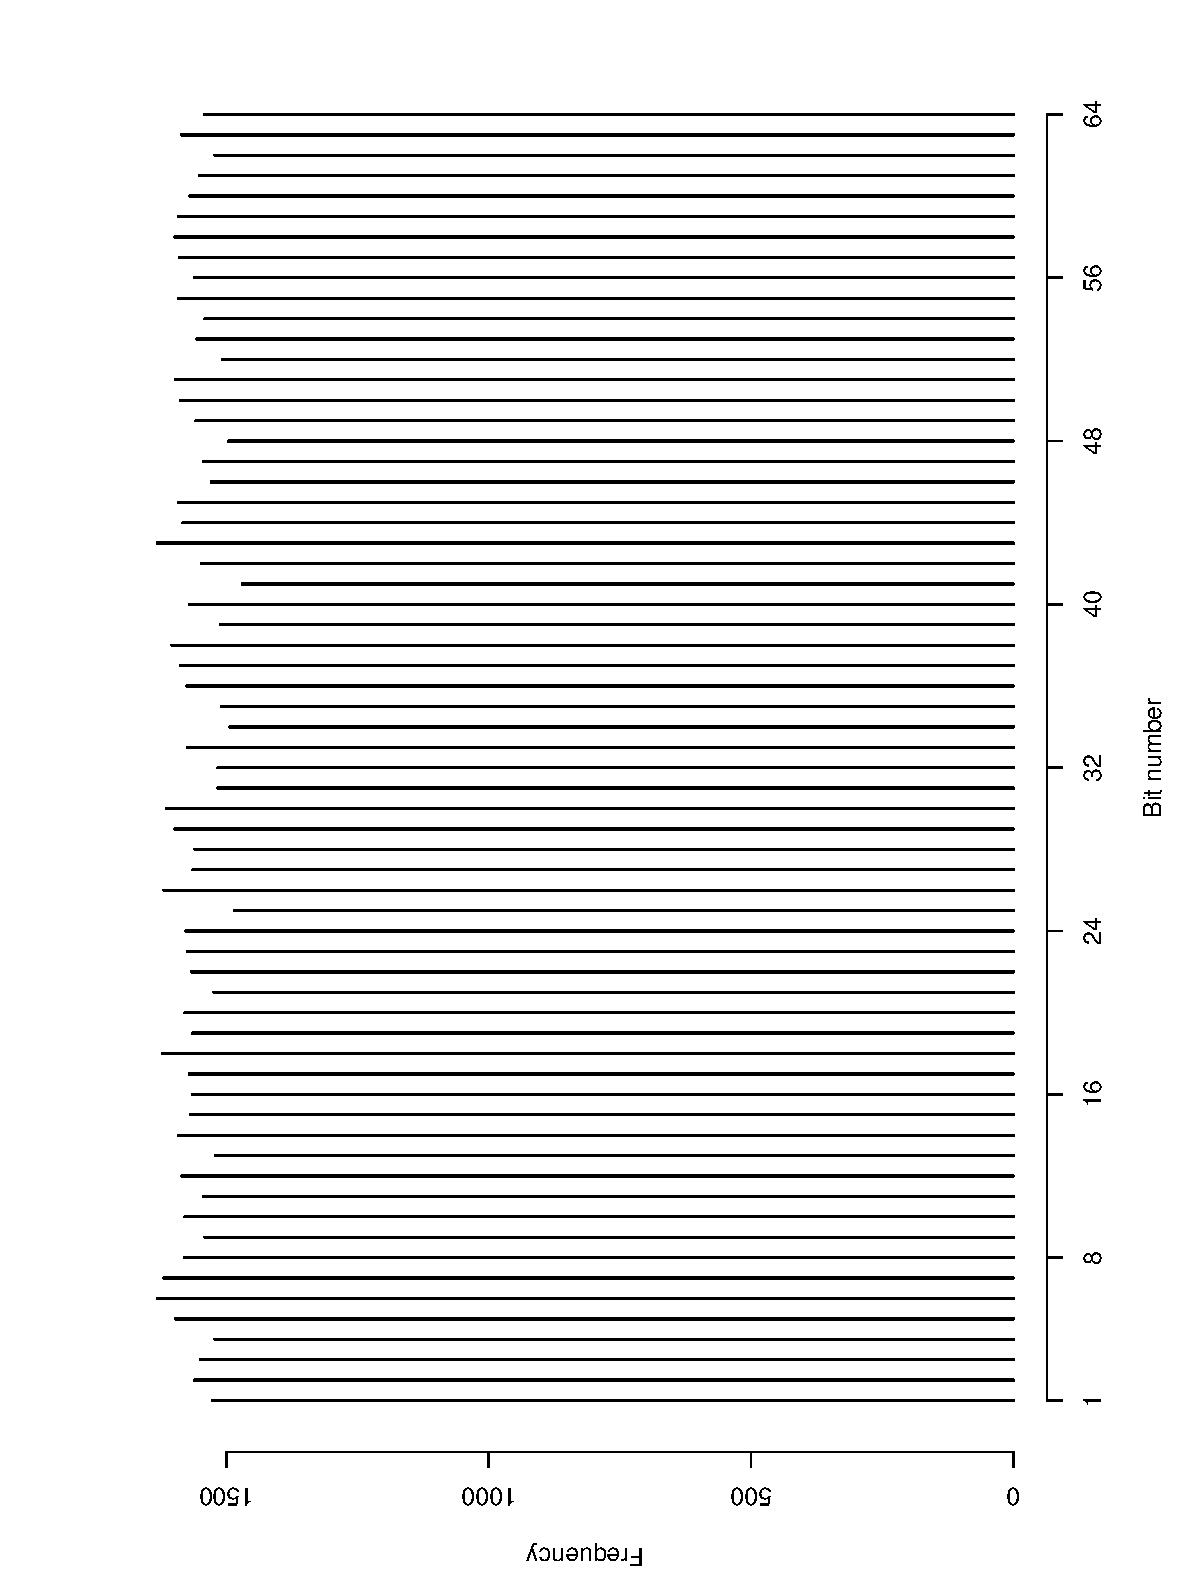
\includegraphics[scale=0.28,angle=-90]{fig10}
  }
  \subfigure[$\alpha_1=16,\beta_1=46,\alpha_2=49,\beta_2=64$]{
  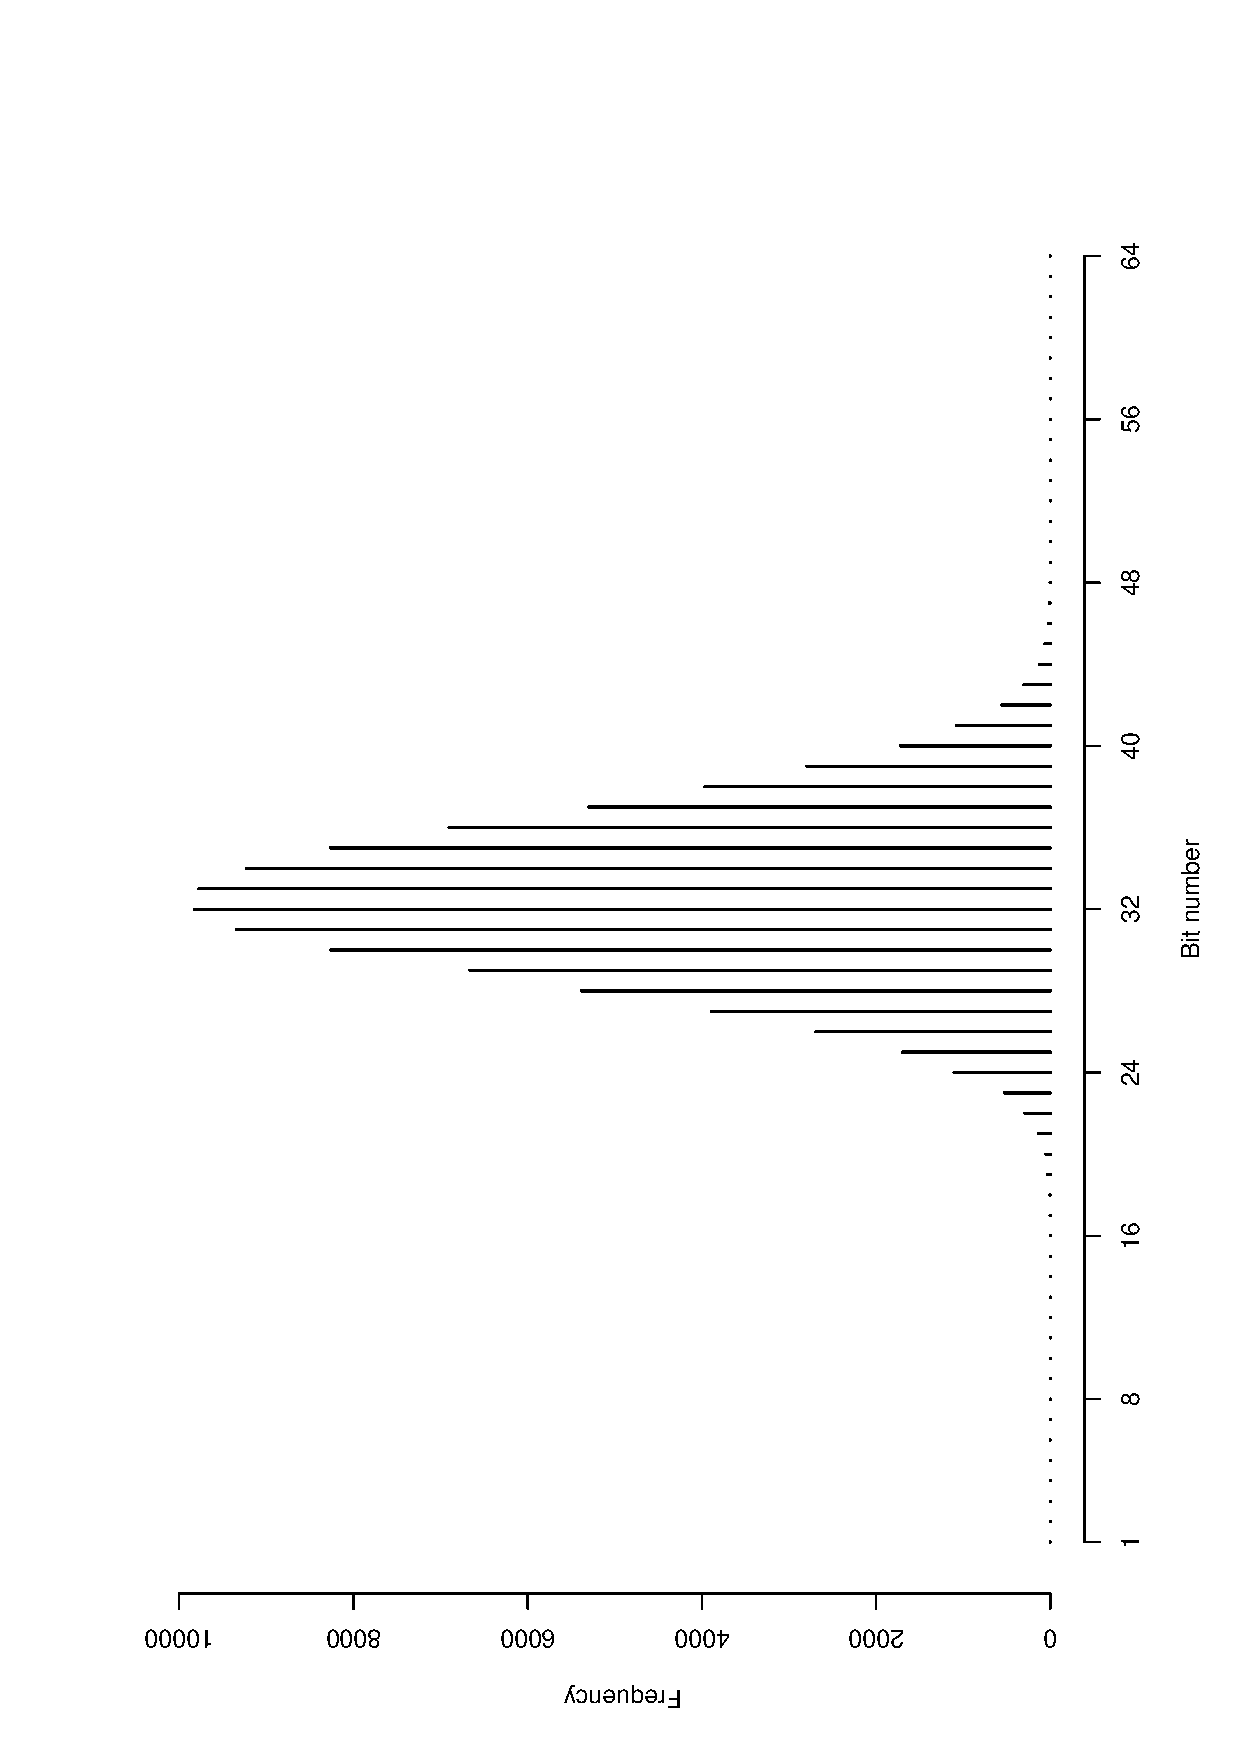
\includegraphics[scale=0.28,angle=-90]{fig11}
  }
  \subfigure[$\alpha_1=16,\beta_1=16,\alpha_2=16,\beta_2=49$]{
  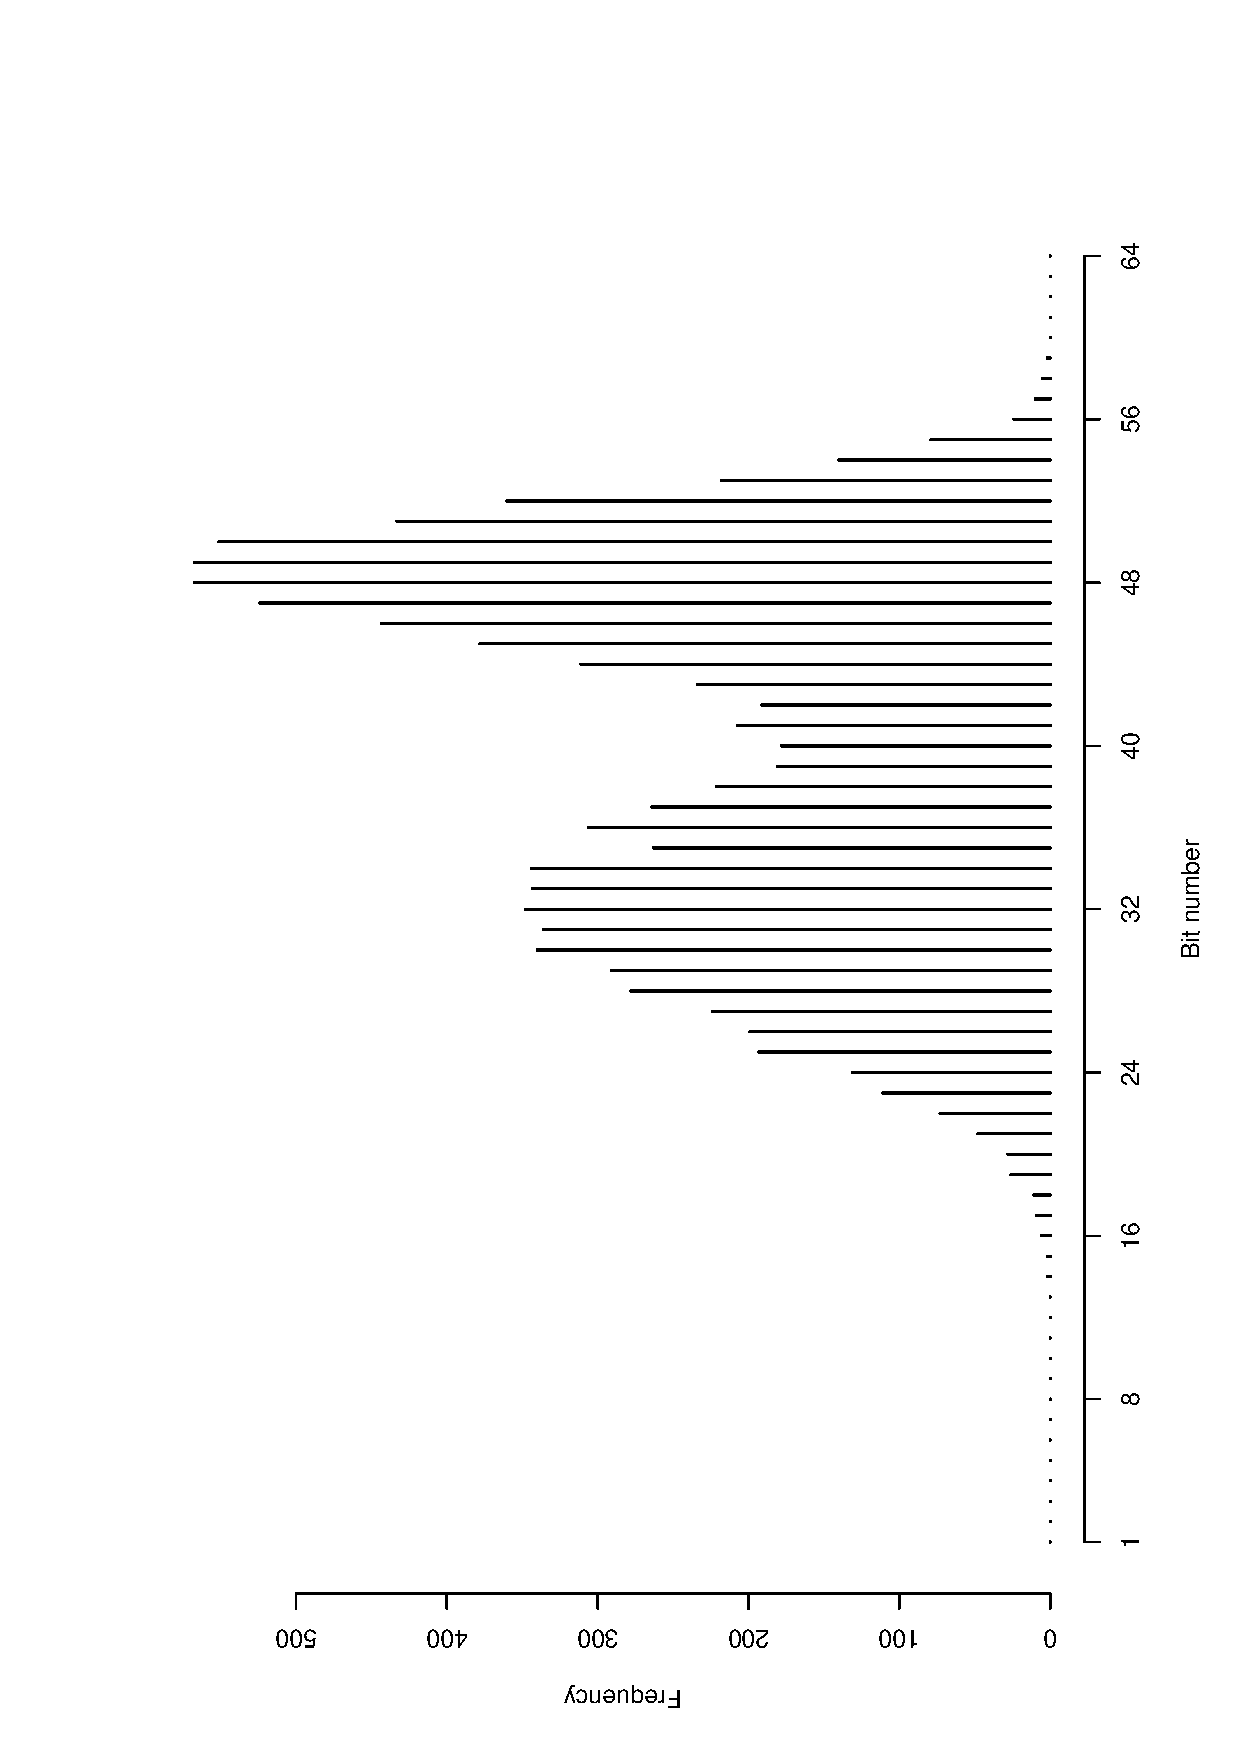
\includegraphics[scale=0.28,angle=-90]{fig12}
  }
  \subfigure[$\alpha_1=1,\beta_1=16,\alpha_2=1,\beta_2=49$]{
  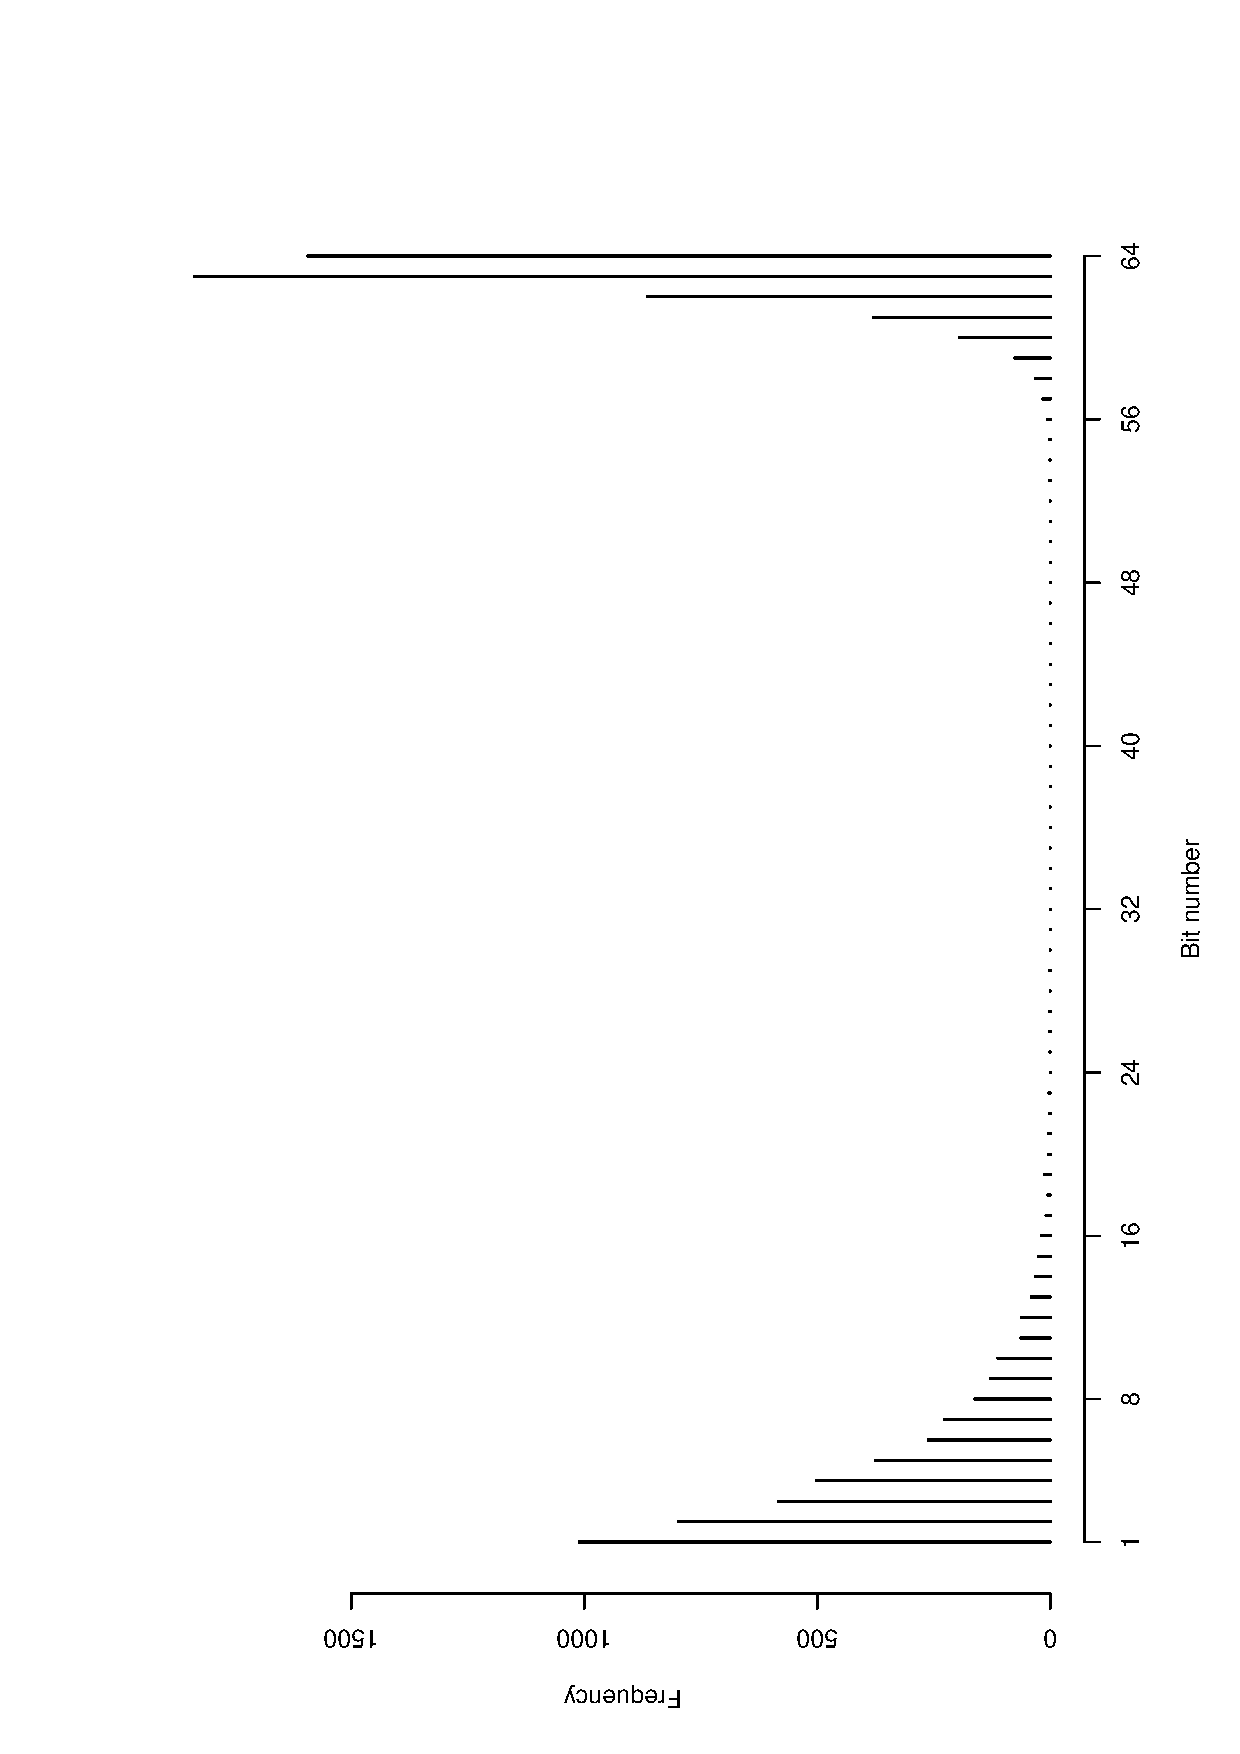
\includegraphics[scale=0.28,angle=-90]{fig13}
  }
  \caption{Histograms constructed from samples with 10,000 elements, generated from the combination of two distributions Betas. Below each histogram is possible to verify the parameters used.}
  \label{fig:02B}
\end{figure}

\begin{table}[h]
 \centering
 \caption{Efficiency comparison in the compression data process methods I and II for sample data generated from a mixture of beta distributions parameterized alphas and betas. It was enumerated methods in which each method was more efficient.}
 \begin{tabular}{ccc}
  \hline 
  Methods  & Sample   & Percentage \\
  \hline
  I	   & 592	& 0.9034\% \\
  II	   & 64944	& 99.0966\% \\
  \hline
  Total    & 65536	& 100\% \\
  \hline
 \end{tabular}
 \label{tab:06}
\end{table}

\begin{figure}[h]
  \centering
  \subfigure[Efficiency histogram of the method I]{
  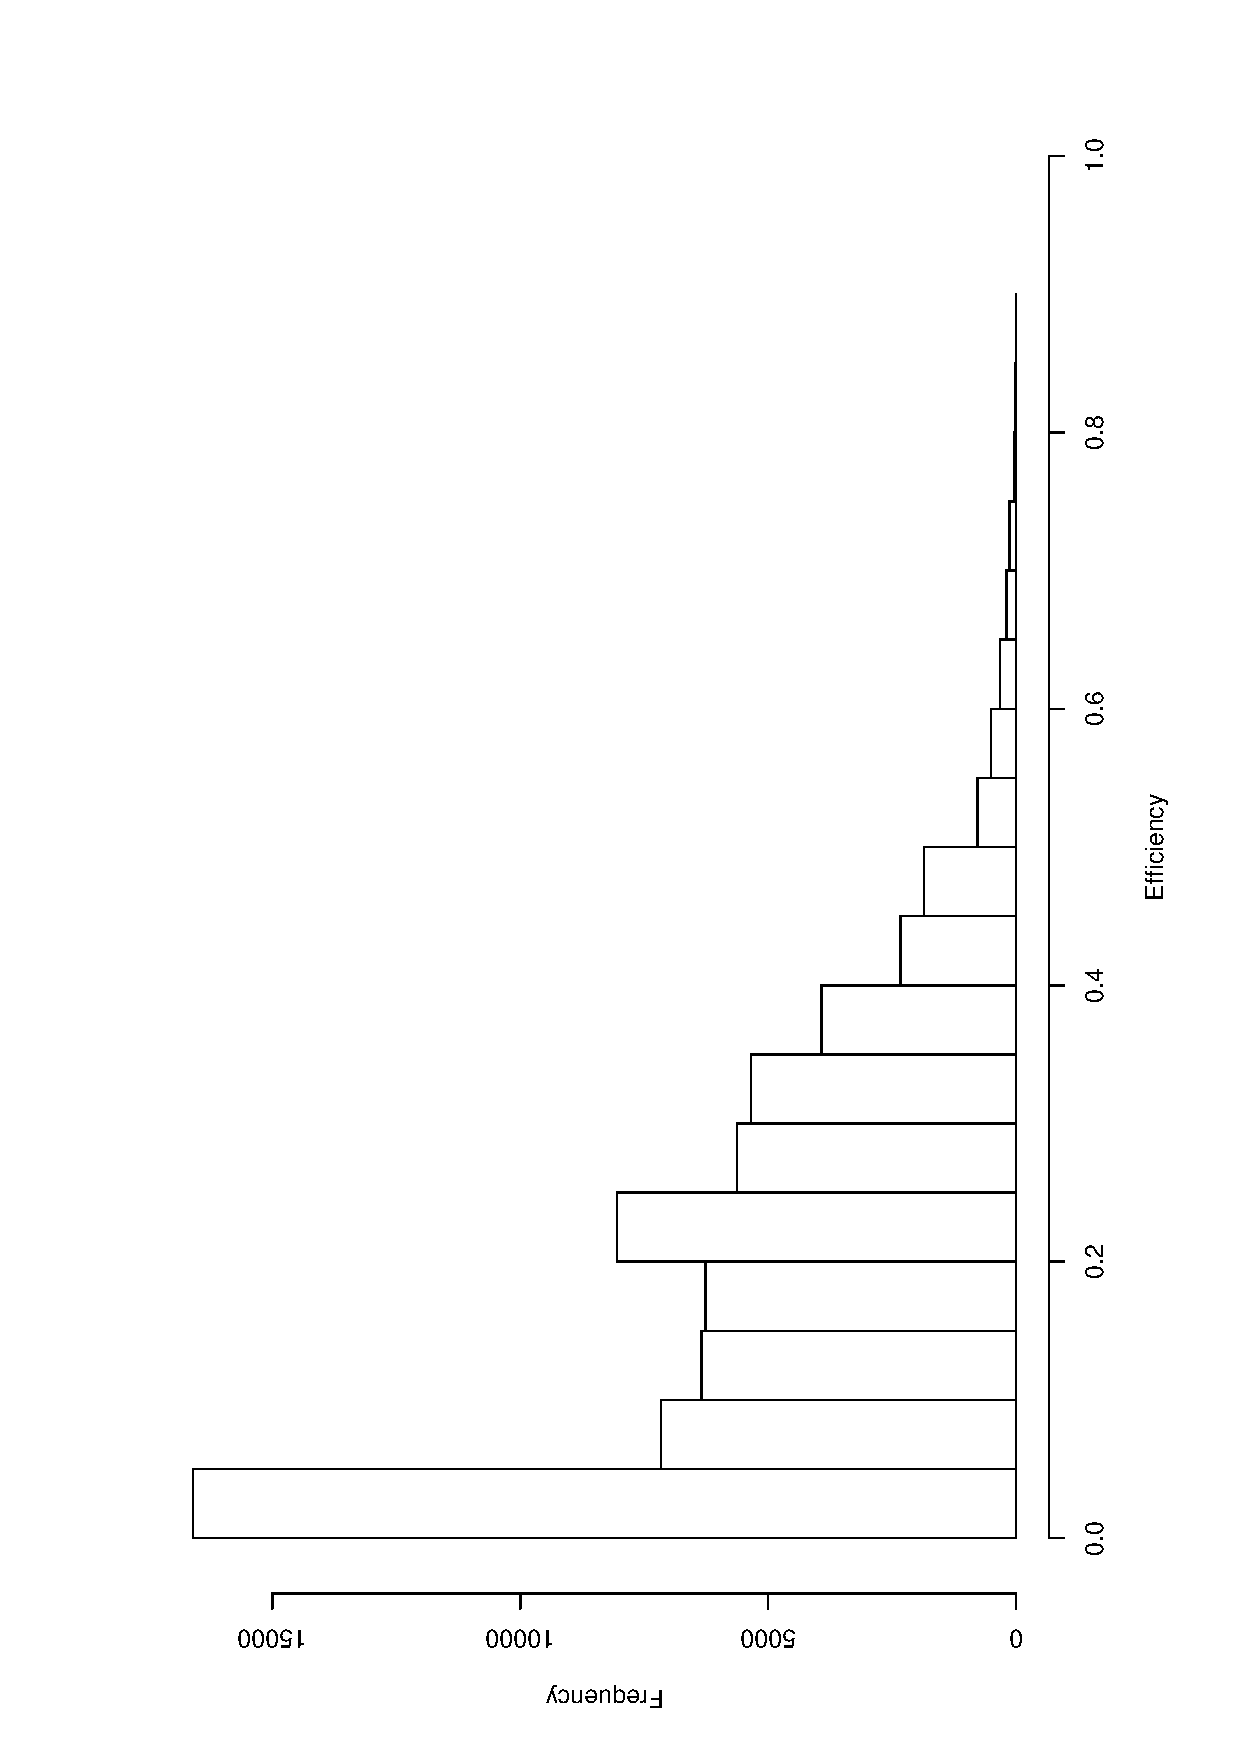
\includegraphics[scale=0.4,angle=-90]{fig14}
  \label{fig14}
  }
  \subfigure[Efficiency histogram of the method II]{
  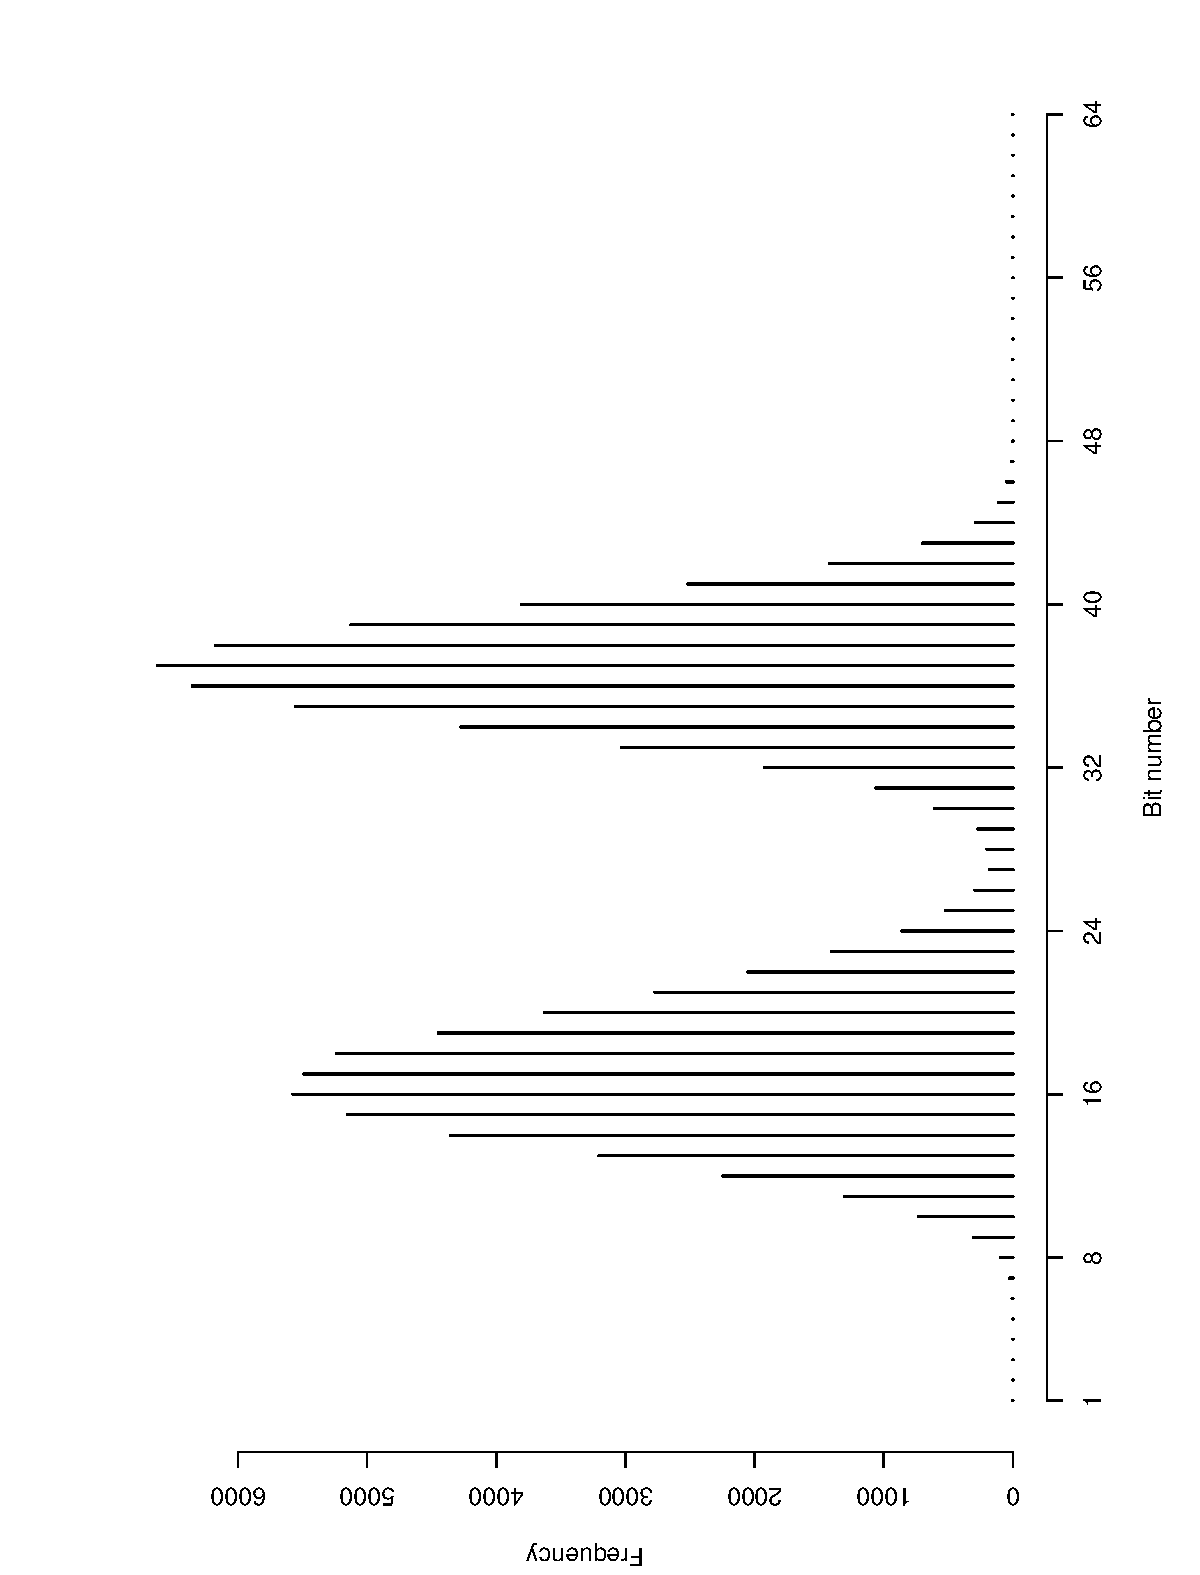
\includegraphics[scale=0.4,angle=-90]{fig15}
  \label{fig15}
  }
  \caption{Efficiency histograms of the methods I and II. It is verified that the method II gives an average efficiency greater than method I.}
  \label{fig:1415}
\end{figure}

\begin{figure}[h]
  \centering
  \subfigure[Efficiency of the methods I and II as a function of the mean distributions mixed.]{
  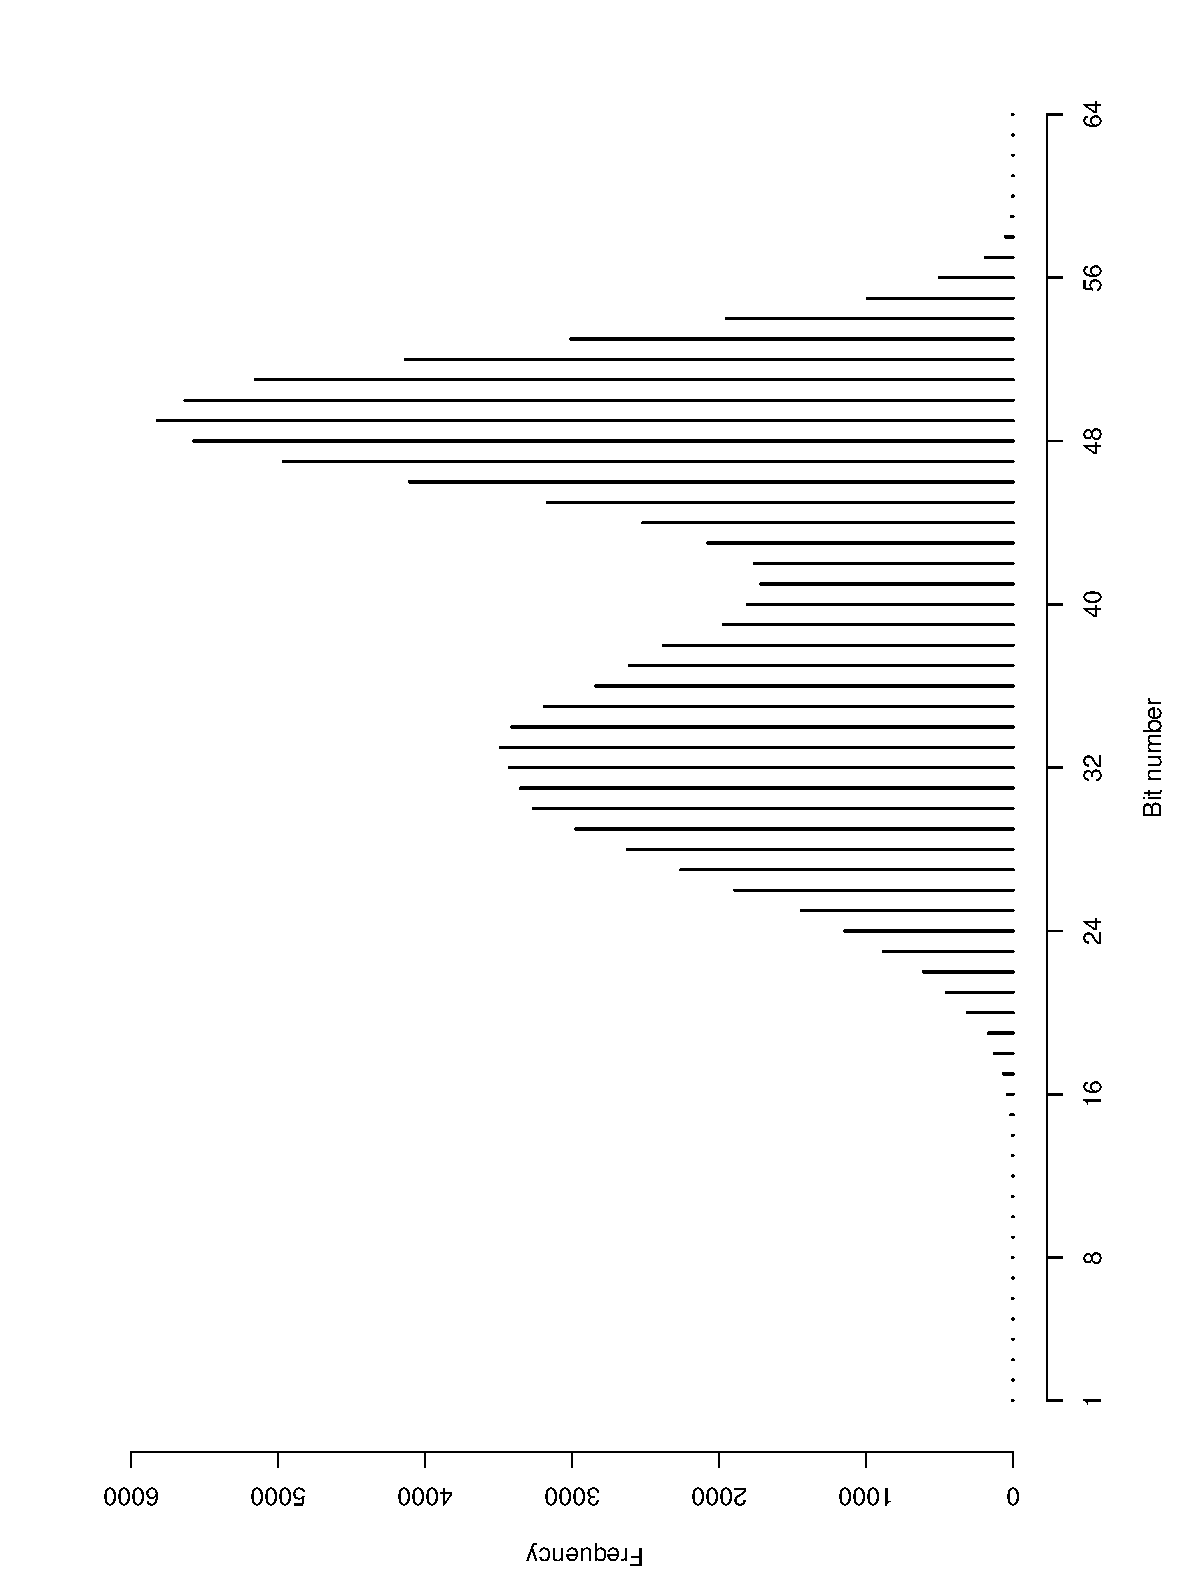
\includegraphics[scale=0.4]{fig16}
  \label{fig16}
  }
  \subfigure[Efficiency of the methods I and II as a function of the variance distributions mixed.]{
  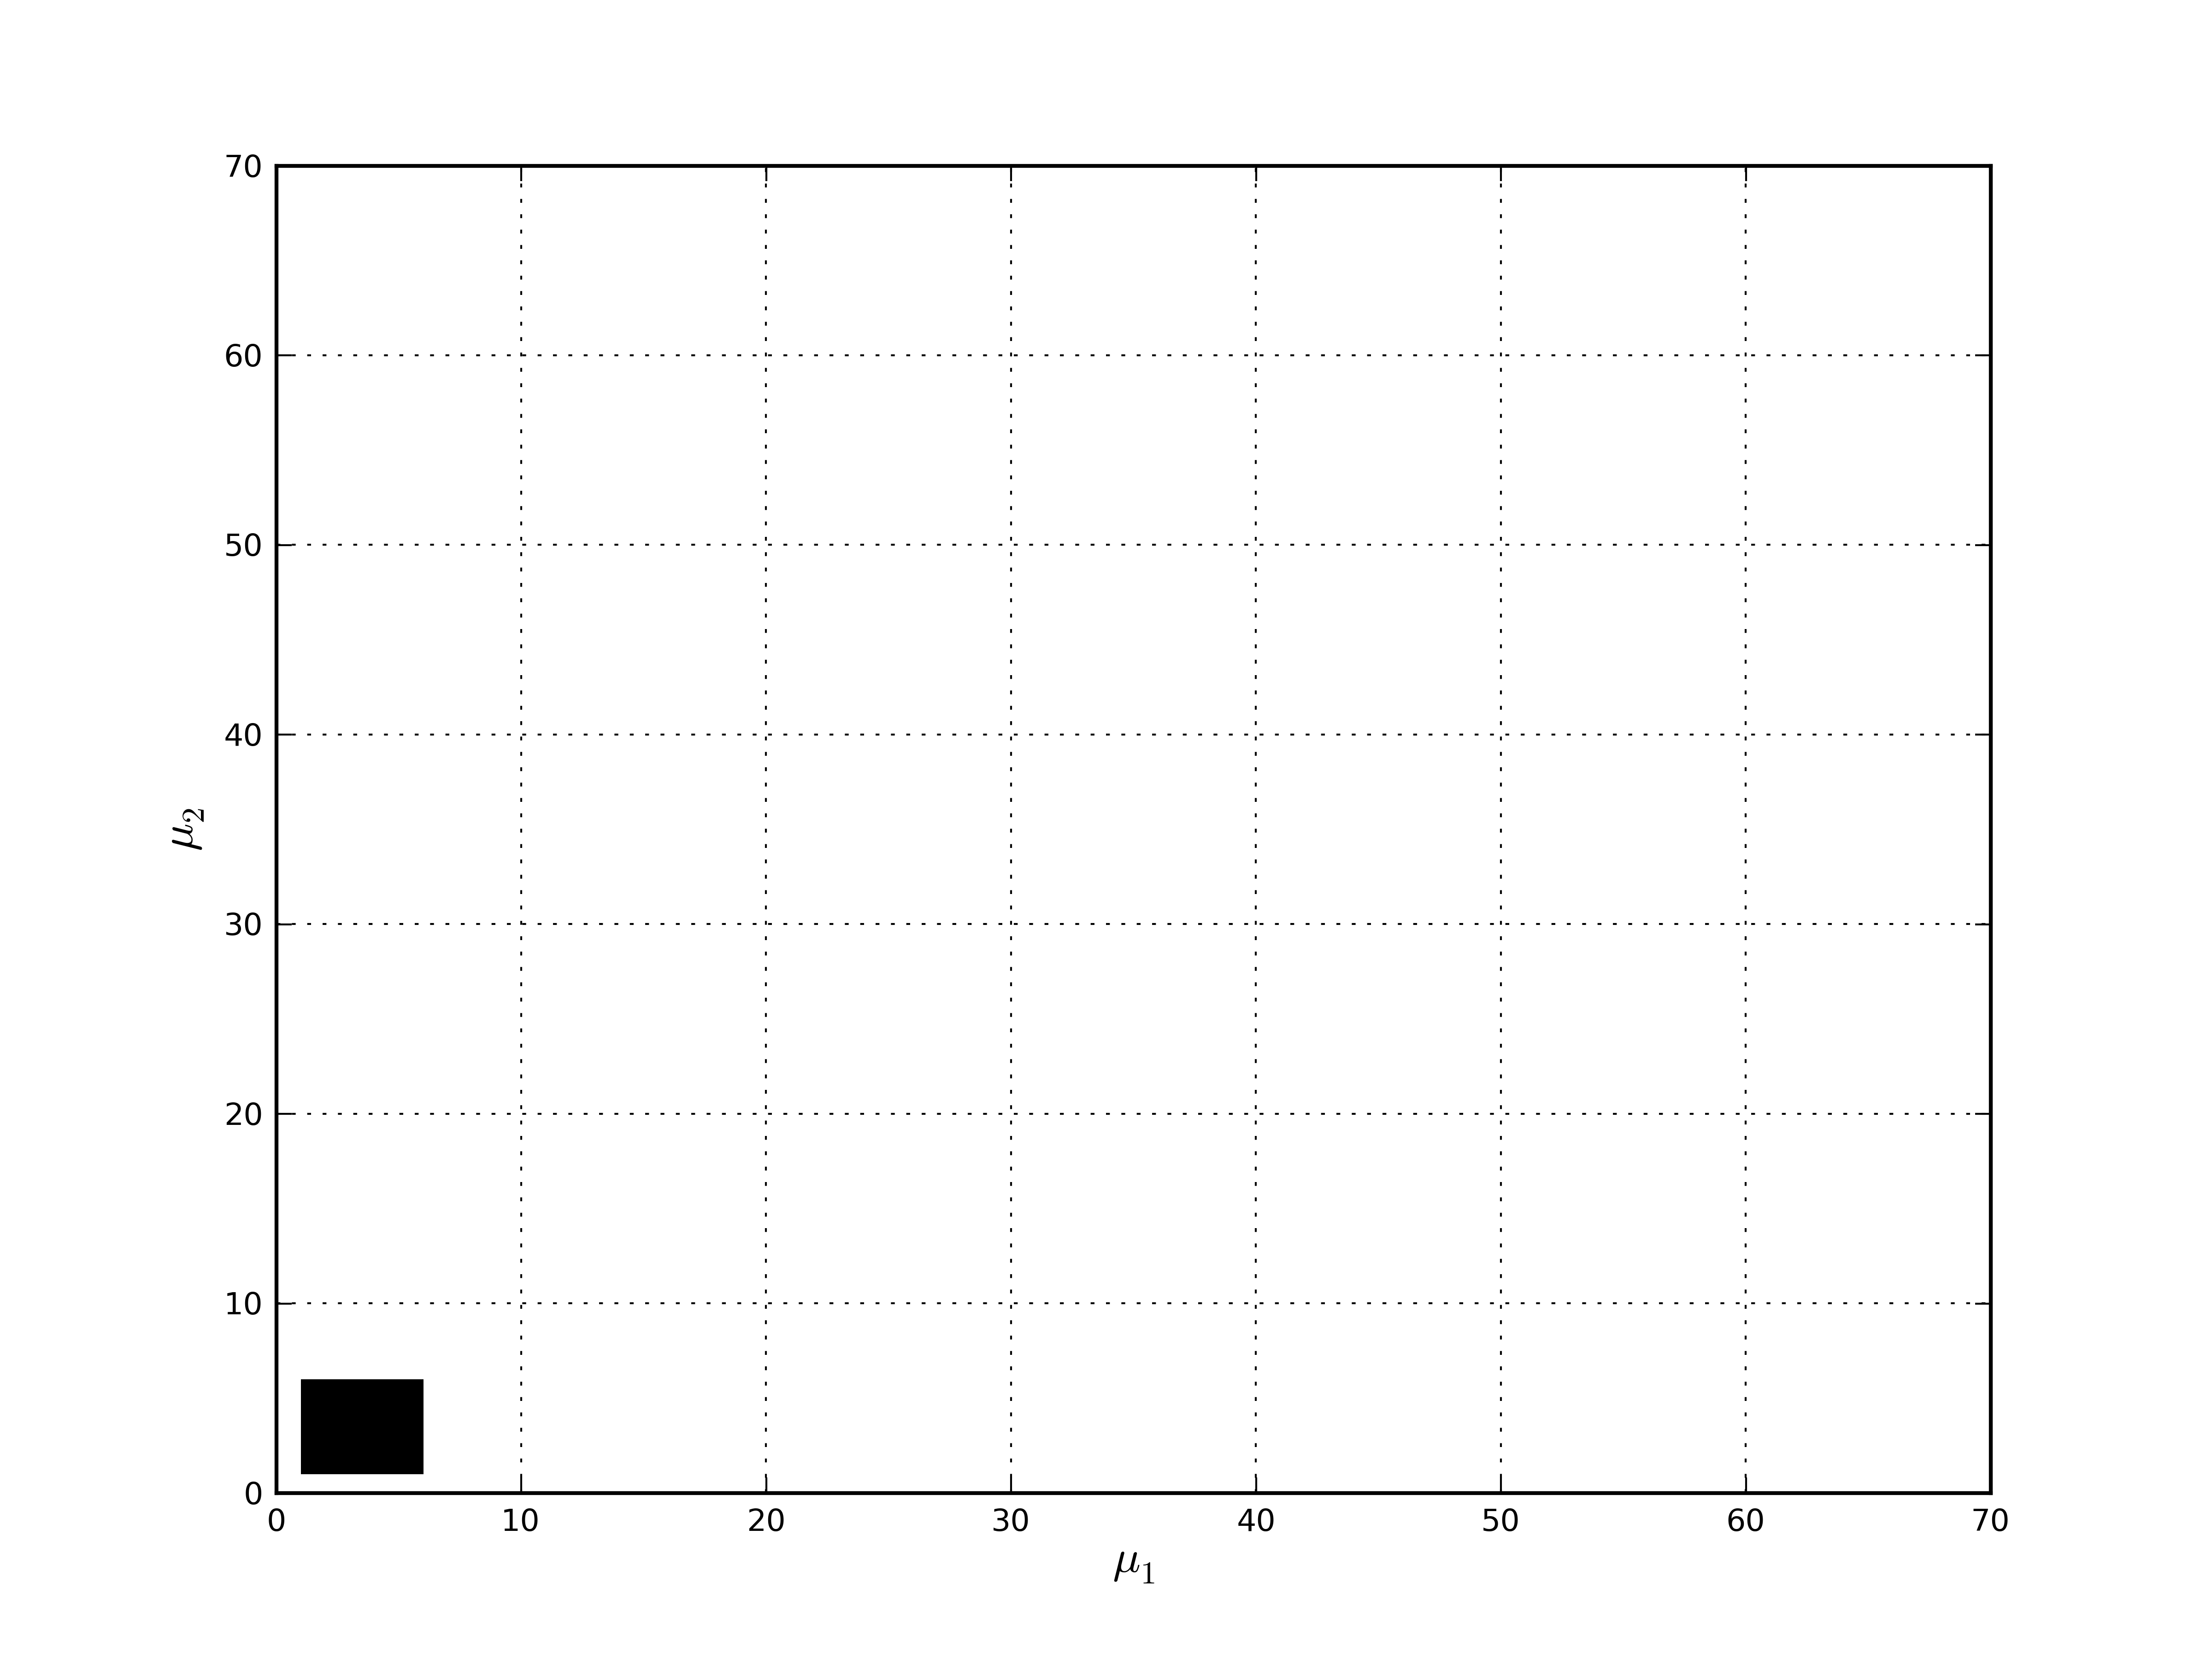
\includegraphics[scale=0.4]{fig17}
  \label{fig17}
  }
  \caption{Mean values ​​of the distributions mixed in which method I and II are more efficient. Note that only a small region with high values ​​for the mean distributions mixed that the method  I is more efficient, in other regions the method II is highlighted. With respect to variance of distributions mixed, one can verify that the method I is more efficient for low values ​​of the variance.}
  \label{fig:1617}
\end{figure}

% Até o momento, o método 2 é mais eficaz no processo de compressão dos dados. Isso ocorre, pois caso exista alguma variância no conjunto de dados da matriz M, o método 2 consegue reduzir a perda dos bits desnecessários para representar alguns números, promovendo a economia dos bits. Existem casos nos quais a variância entre os números é nula ou infíma. Nesses casos, o método 1 é mais eficaz, pois para um mesmo número de bits, pode-se representar diferentes números, por exemplo, com 3 bits é possível representar os valores de 0 até 7. Portanto, caso uma matriz seja constituídas por valores entre 0 e 7, o método 1 será mais eficaz, pois irá representar os números por meio de um número menor de bits. Para simular a situação descrita e as outras com as mesmas caracterísicas foi realizado uma simulação, gerando 10,000 valores para preenncher uma matriz M, de tal forma que esses valores demandem a mesma quantidade de bits para serem representados. Os resultados para essa simulação estão representados nas Figuras \
% ref{fig18} e \ref{fig19}. Na Figura \ref{fig18} pode-se verificar que o método 1 é mais eficiente no processo de compressão dos valores da matriz M para diferentes números de bits, pois não existem diferenças entre os números de bits necessários para representar cada um dos valores dos elementos da matriz M. Como possuem a mesma quantidade de bits, o método 1 torna-se mais eficaz nesse caso. Na Figura \ref{fig19}, pode-se observar o comportamento da diferença da eficiência entre os dois métodos em função do número de bits. Nessa figura é possível verificar que a medida que os valores são representados por mais bits, o método 1 é mais eficiente, mas quando os valores se aproximam de 64 bits, caem buscamente. Essa queda ocorre que quando o número de bits atinge o valor 64, nenhum dos dois métodos é eficaz para representar os valores, e portanto não existe compressão dos dados. Vale ressaltar que com esse experiment, o método II não foi mais eficaz em nenhuma situação do que o método I.

Until now, the method 2 is more effective in the data compression process. This occurs, because if there is some variance in the data set matrix M, the second method can reduce the unnecessary bits loss to represent some numbers, promoting the bit economy. There are cases where the variance between the numbers is null or insignificant. In such cases, the first method is more efficient, since for the same bit number can represent different numbers, for example, 3 bits can represent the values ​​0 through 7. Therefore, if one matrix is ​​constituted by values ​​between 0 and 7,  method I would be more efficient to represent the numbers by a smaller bit number. To simulate the situation described above and the other with the same characteristics a simulation was carried out, generating 10,000 values ​​for a matrix M, so that these values ​​demanding the same amount of bits to be represented. The results for this simulation are shown in Figures \ref{fig18} and \ref{fig19}. In Figure \ref{fig18} can be verified that the first method is more efficient in the compression process of the matrix M values ​​for different bit numbers since there are no differences between the bit numbers required to represent each element value of the matrix M. Since they have the same bit number, the first method becomes more effective in this case. In Figure \ref{fig19}, we can observe the behavior of the difference in efficiency between the two methods depending on the bit number. In this picture you can see that the measured values ​​are represented by more bits, method 1 is more efficient, but when the values ​​are close to 64-bit, decrease sharply. This decrease occurs when the bit number reaches the value 64, neither method is effective to represent the values​​, and so there is no compression of the data. It is noteworthy that in this experiment, the method II was no more effective in any situation than method I. 

\begin{figure}[h]
  \centering
  \subfigure[Comparison of the efficiency of the methods I e II.]{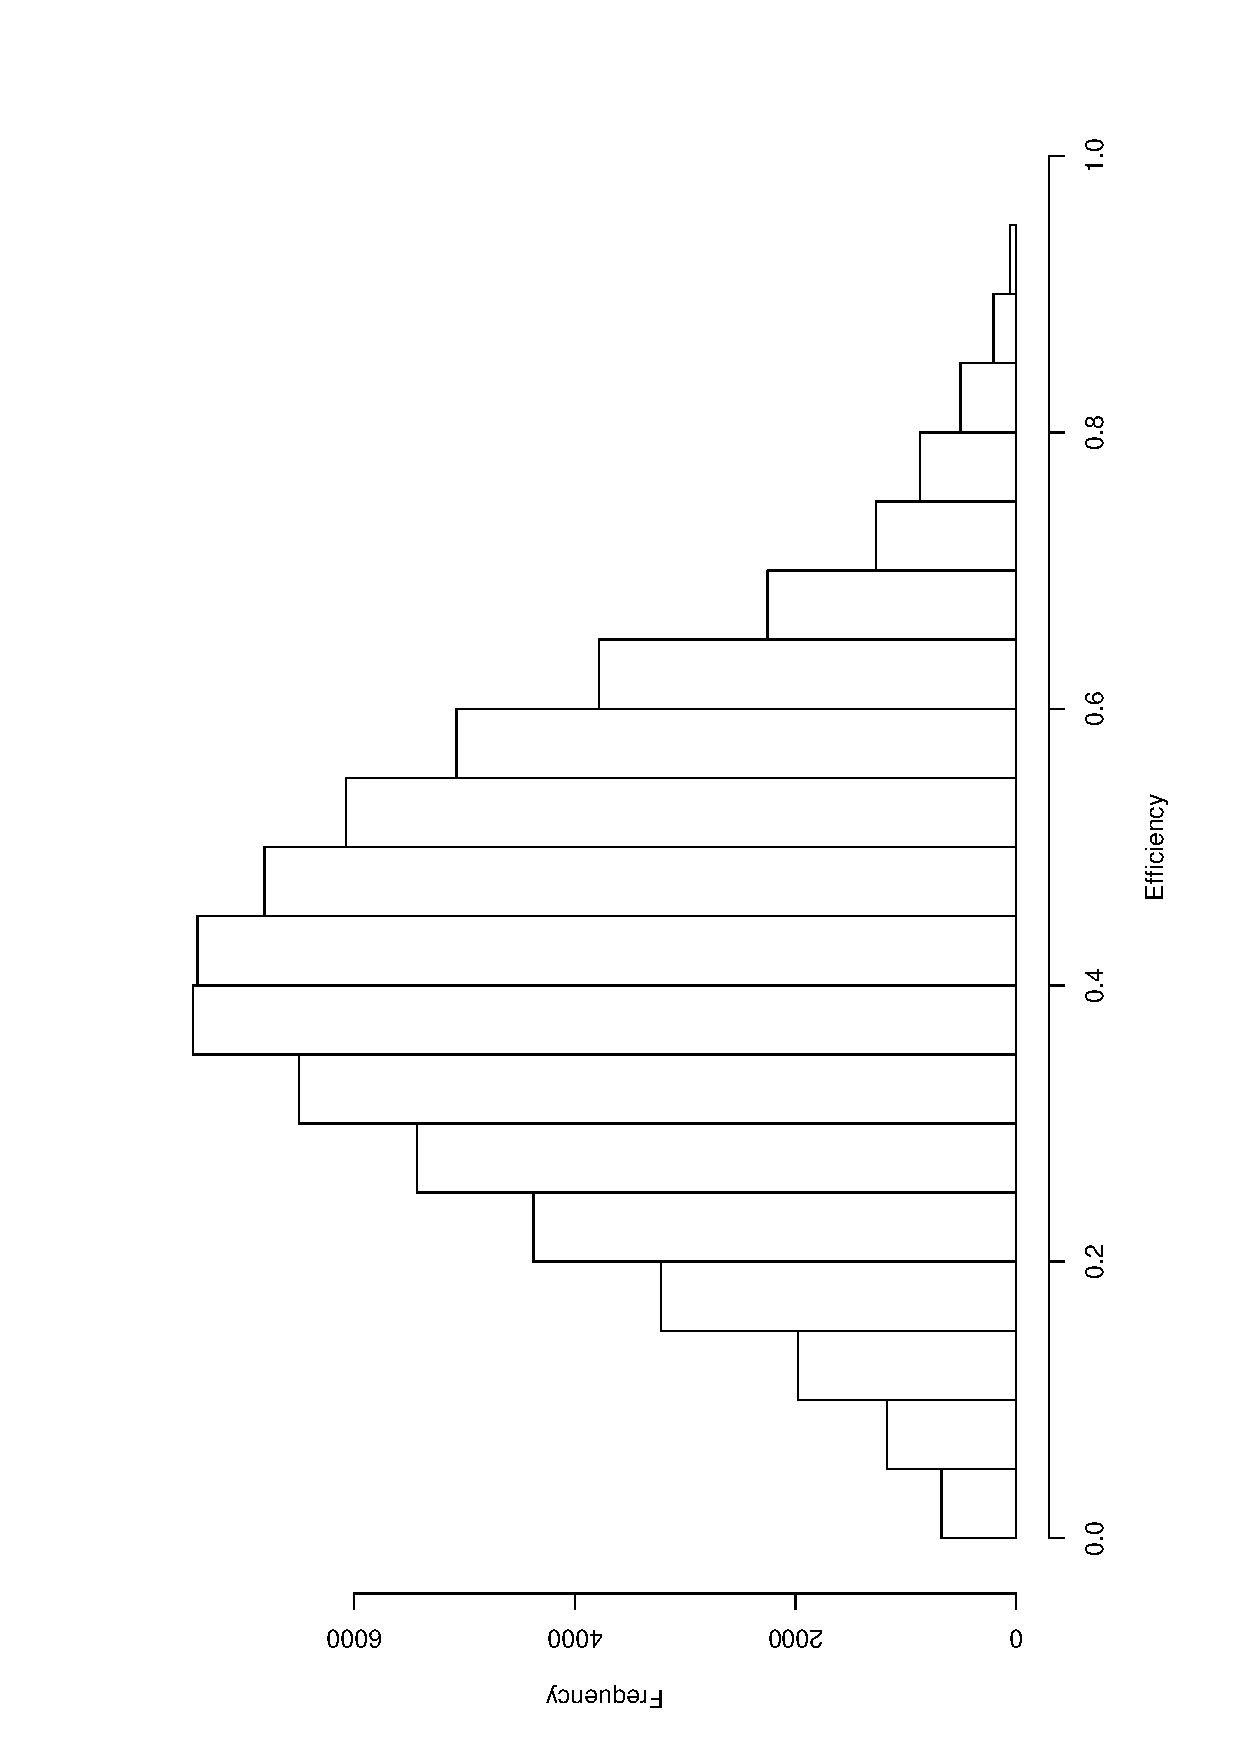
\includegraphics[scale=0.3]{fig18}\label{fig18}}
  \subfigure[Difference in efficiency of the methods I e II.]{\includegraphics[scale=0.3]{fig19}\label{fig19}}
  \caption{Efficiency of the methods I and II the data compression process of a matrix of numbers which require the same amount of bits to be represented.}
  \label{fig:1819}
\end{figure}
  
% A simulação realizada anteriormente, ocorre em casos muitos específicos, mas mesmo assim, o método I consegue comprimir os valores gerados. Agora vamos analisar o comportamento do processo de compressão realizados sobre amostras geradas a partir da mistura de dois conjunto de dados. Os valores gerados para cada conjunto de dados, que juntos totalizam 10,000 valores, formam a matriz M. Todos os valores são representados por meio de duas quantidade de bits, sendo definidas como $b_1$ e $b_2$ para os métodos 1 e 2, respectivamente. A diferença agora é que existe um $\lambda$, que define a quantidade de elementos de cada grupo para formar a matriz M (Equação \ref{eq:61}).

The simulation performed previously, occurs in very special cases, but even so, the method I can compress values ​​generated. Now, let us consider the behavior of the compression process performed on samples generated from the mixing of two dataset. The values ​​generated for each set of data, which together total 10,000 values, forming the matrix M. All values ​​are represented by two bit quantity and is defined as $B_1$ and $B_2$ to methods I and II, respectively. The difference now is that there is a $\lambda$, which defines the element number in each group to form the matrix M (Equação \ref{eq:61}).

\begin{equation}\label{eq:61}
  n = \lambda b_1 + (1-\lambda) b_2
\end{equation}

% Os resultados podem ser verificados na Figura \ref{fig:2125}. Nas Figuras \ref{fig20}, \ref{fig22} e \ref{fig24}, pode-se verificar as superfícies que descrevem o compormento da eficiência dos processos 1 e 2 para os valores de $\lambda=0.1$, 0.5 e 0.9, respectivamente. Nessas figuras é possível verificar que existe um comportamento constante para o método 1,cujo comportamento da eficiência é crescente para valores próximos ou iguais de $b_1$ e $b_2$, já para os demais valores, nos quais ocorre uma diferença entre o número de bits, a eficiência cai. O método 2, diferente do método 1, apresenta maiores valores de eficiência nas regiões nas quais os número de bits $b_1$ e $b_2$ são discrepantes. A diferença das eficiências dos métodos podem ser verificadas nas Figuras \ref{fig21}, \ref{fig23} e \ref{fig25}. Observe que a curva assume valores positivos para a diferença, logo o método 1 é o melhor. Uma justificativa para esse comportamento é que os números de bits $b_1$ e $b_2$ são próximos. Já para os casos, 
% nos quais os valores de $b_1$ e $b_2$ são discrepantes, o método 2 é o mais eficiente.

The results can be verified in Figure \ref{fig: 2125}. In Figures \ref{fig20}, \ref{fig22} and \ref{fig24}, it can be seen surfaces that describe the behavior of the efficiency of method I and II for the values ​​of $\lambda = 0.1$, 0.5 and 0.9, respectively. In these figures, it can be seen that there is a constant behavior for method I, whose behavior is increasing efficiency to values ​​close or equal to $B_1$ and $B_2$, while for other values​​, where there is a difference between the bit number, the efficiency decrease. The method II, different of the method I, has higher efficiency values ​​in regions where the number of bits $B_1$ and $B_2 $ are discrepant. The difference in the efficiencies of the methods can be verified in Figures \ref{fig21}, \ref{fig23} and \ref{fig25}. Note that the curve takes positive values ​​for the difference, so the method is the best one. A justification for this behavior is that the bit numbers $B_1 $ and $ B_2 $ are close. But for the cases, where the values ​​of $B_1$ and $B_2 $ are discrepant, method II is the most efficient.

\begin{figure}[h]
  \centering
  \subfigure[Comparison of the efficiency of the methods I and II.($\lambda=0.1$)]{
  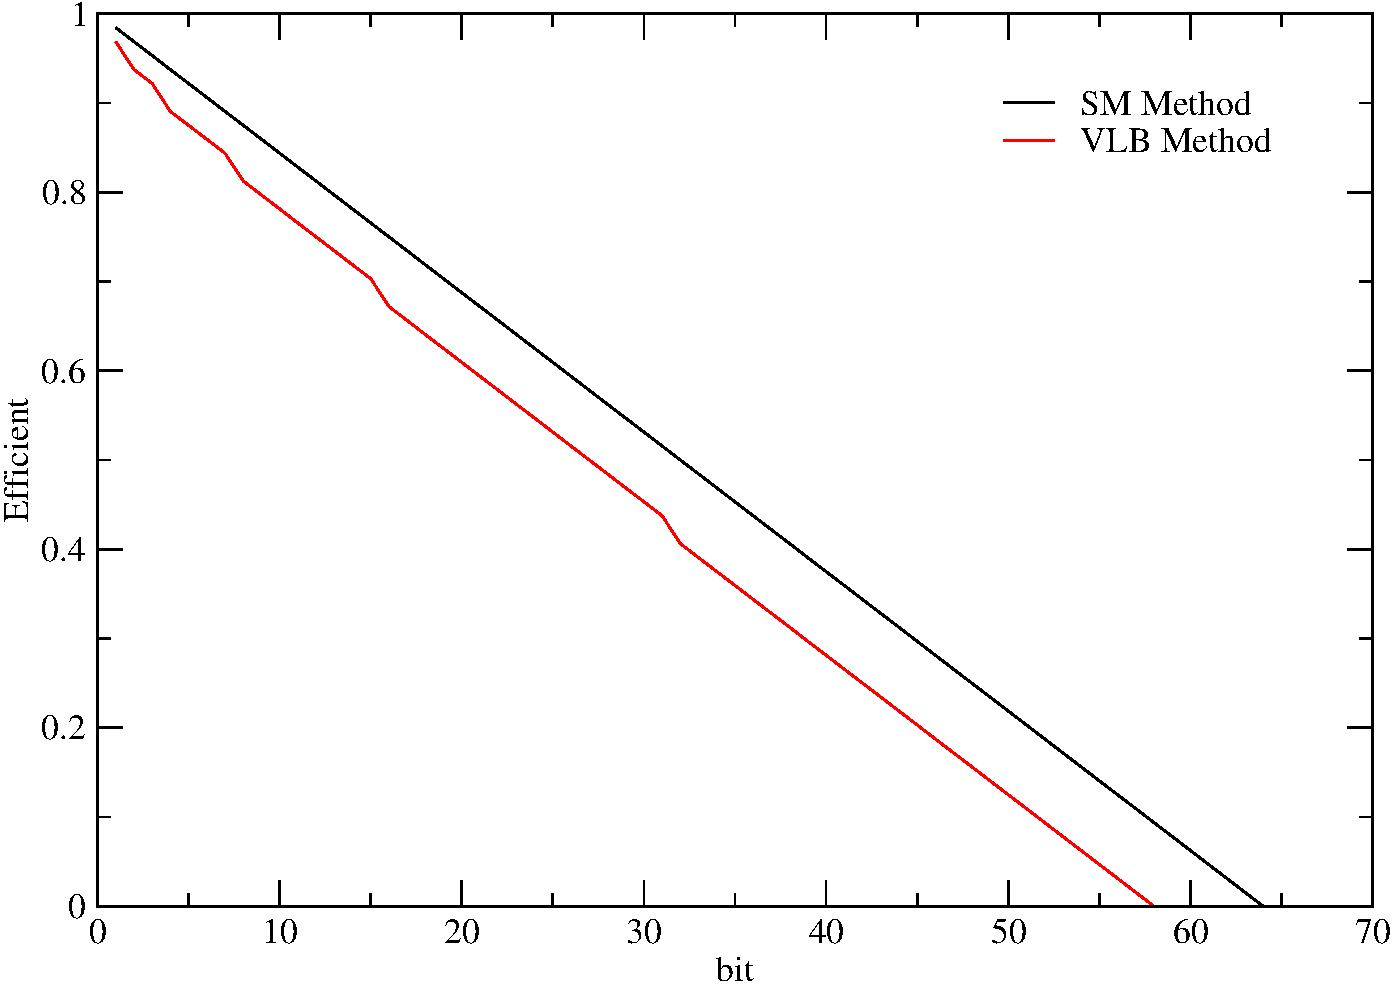
\includegraphics[scale=0.3,angle=-90]{fig20}
  \label{fig20}
  }
  \subfigure[Difference in efficiency of the methods I and II.]{
  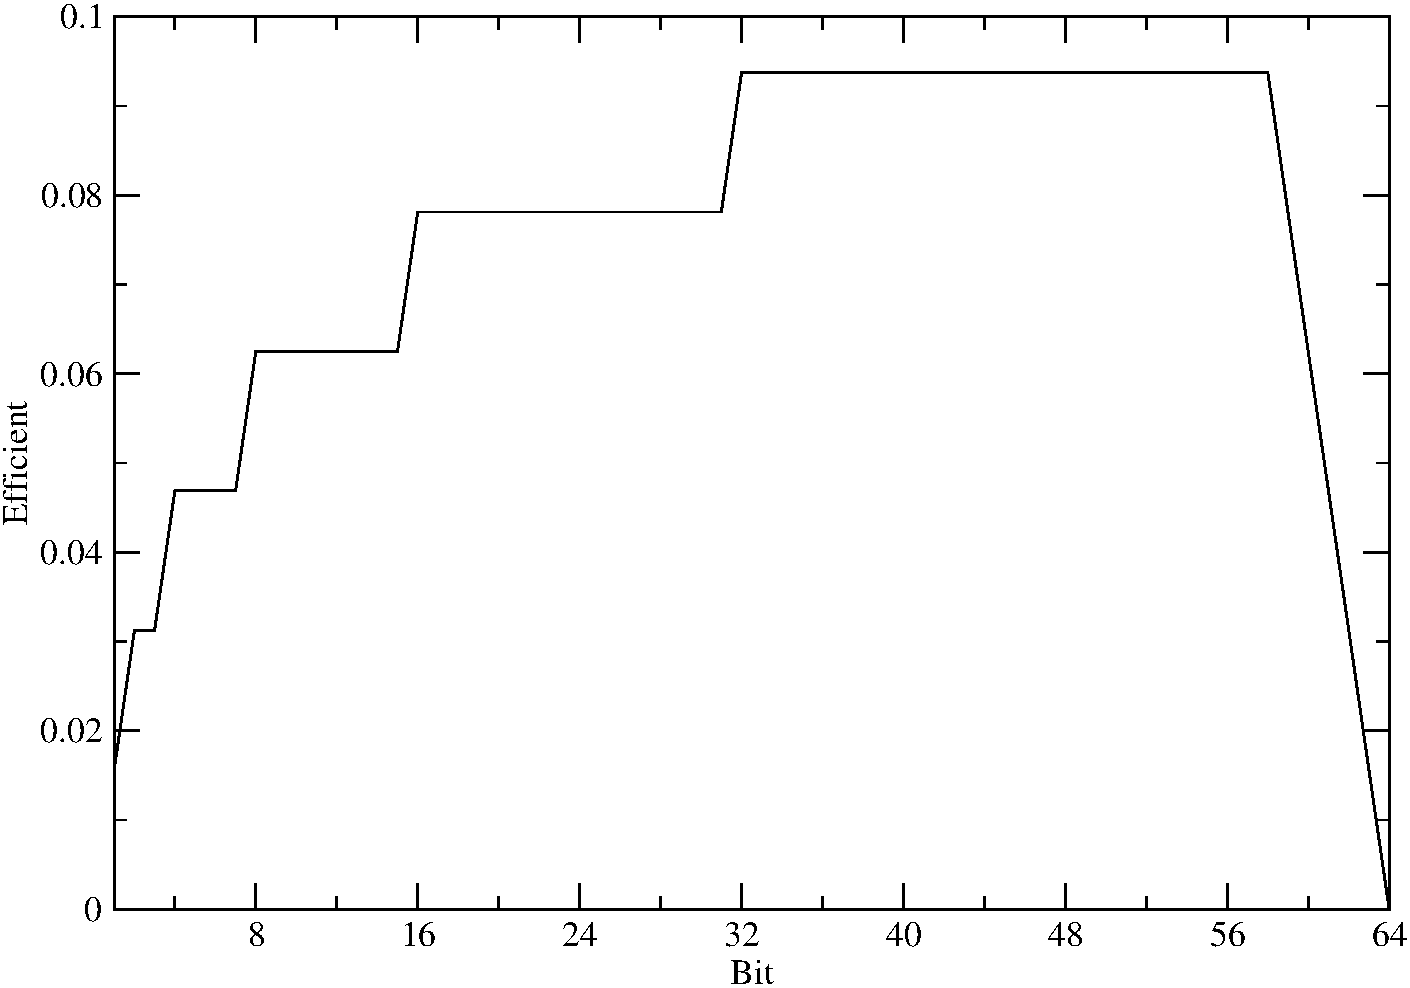
\includegraphics[scale=0.3,angle=-90]{fig21}
  \label{fig21}
  }
  \subfigure[Comparison of the efficiency of the methods I and II.($\lambda=0.1$)]{
  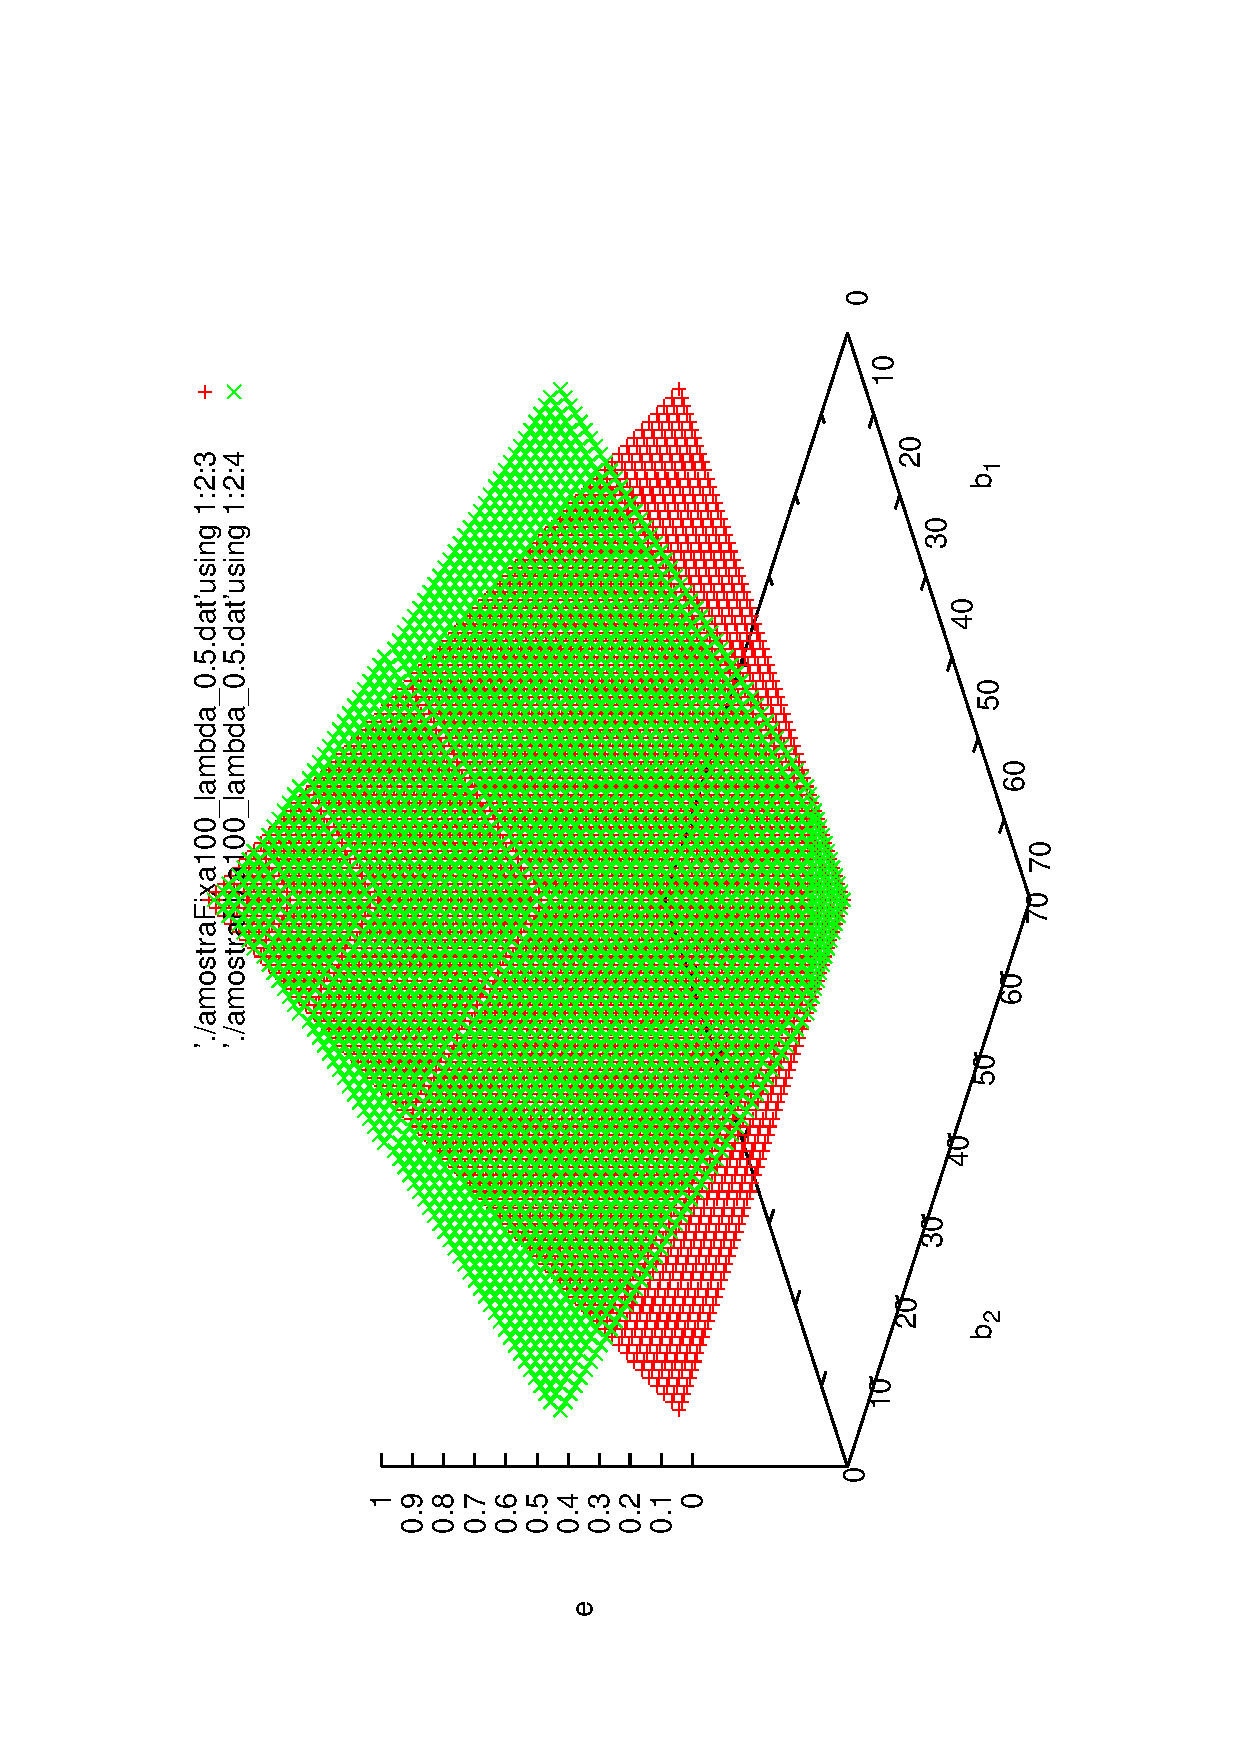
\includegraphics[scale=0.3,angle=-90]{fig22}
  \label{fig22}
  }
  \subfigure[Difference in efficiency of the methods I and II.]{
  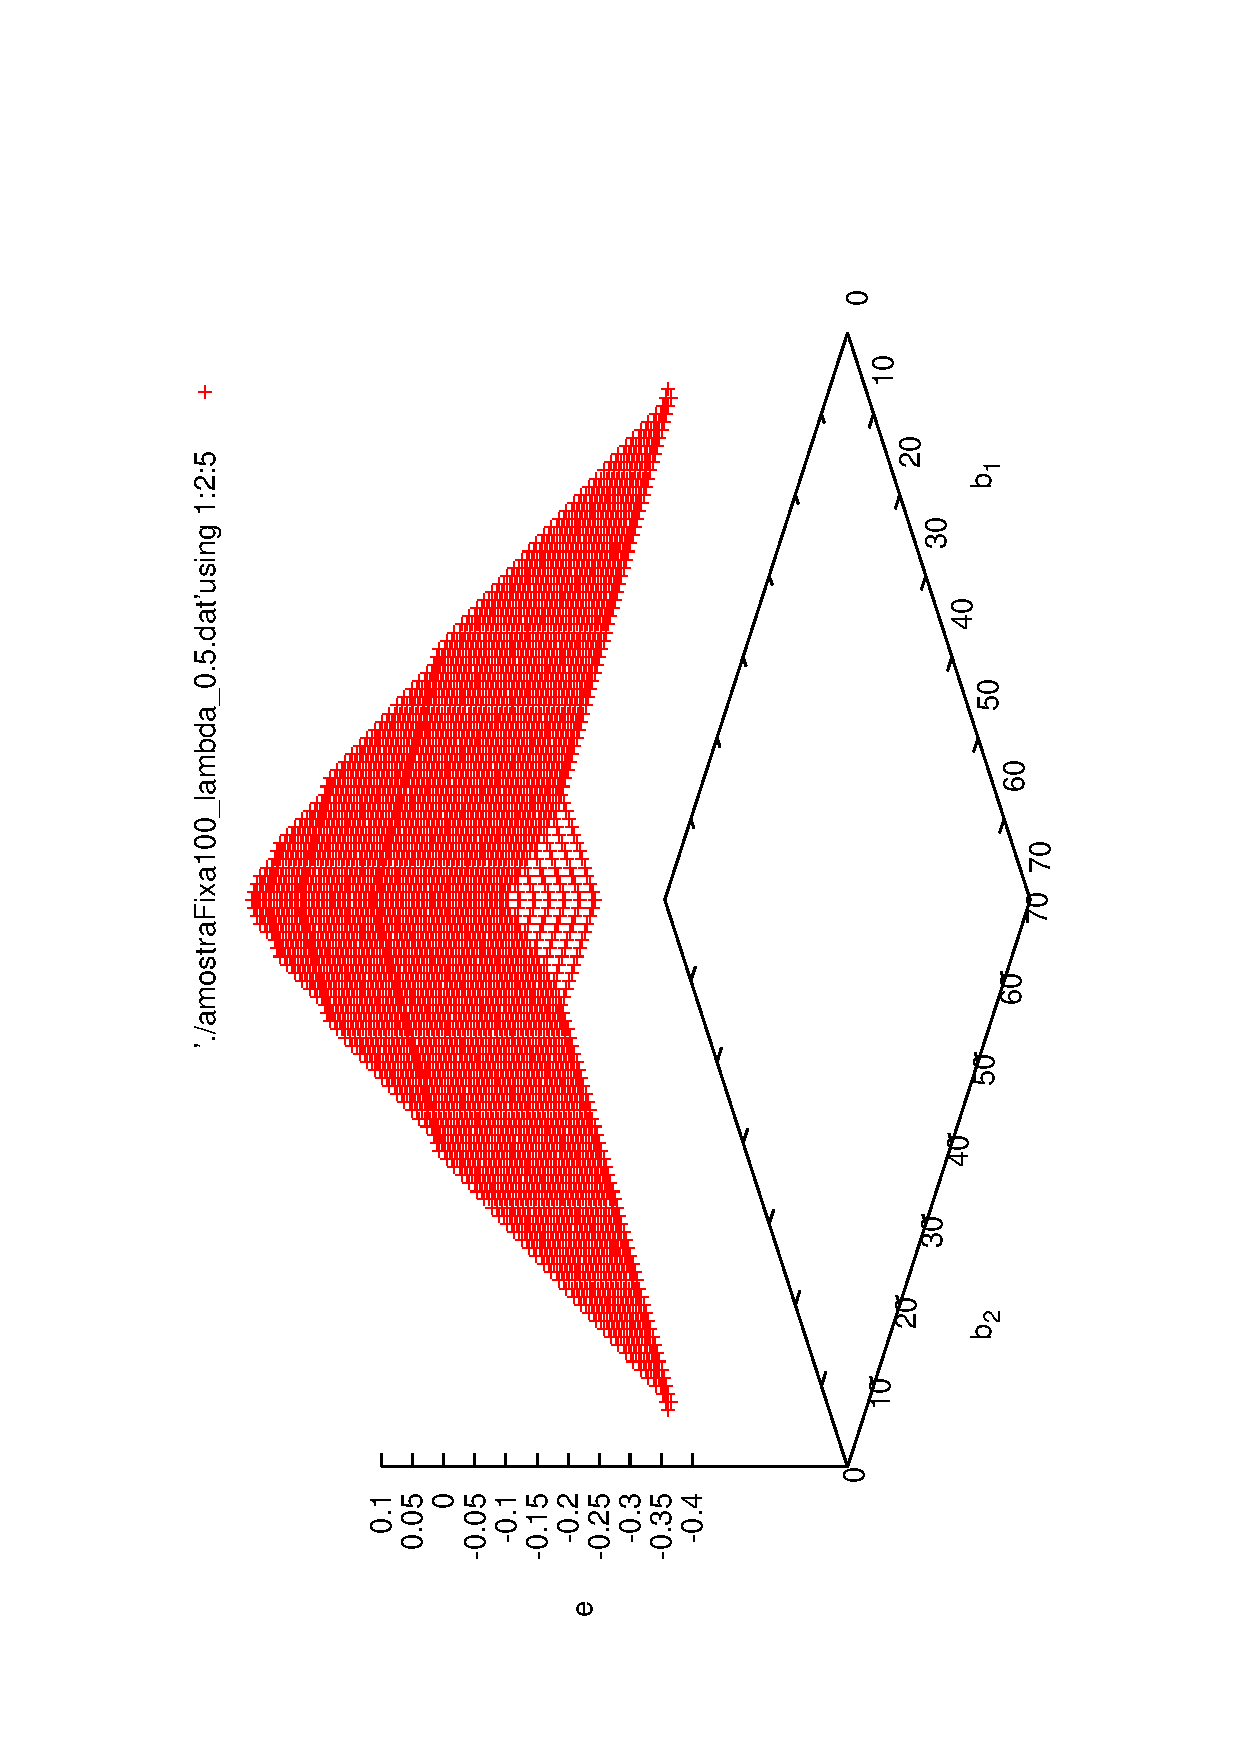
\includegraphics[scale=0.3,angle=-90]{fig23}
  \label{fig23}
  }
  \subfigure[Comparison of the efficiency of the methods I and II.($\lambda=0.1$)]{
  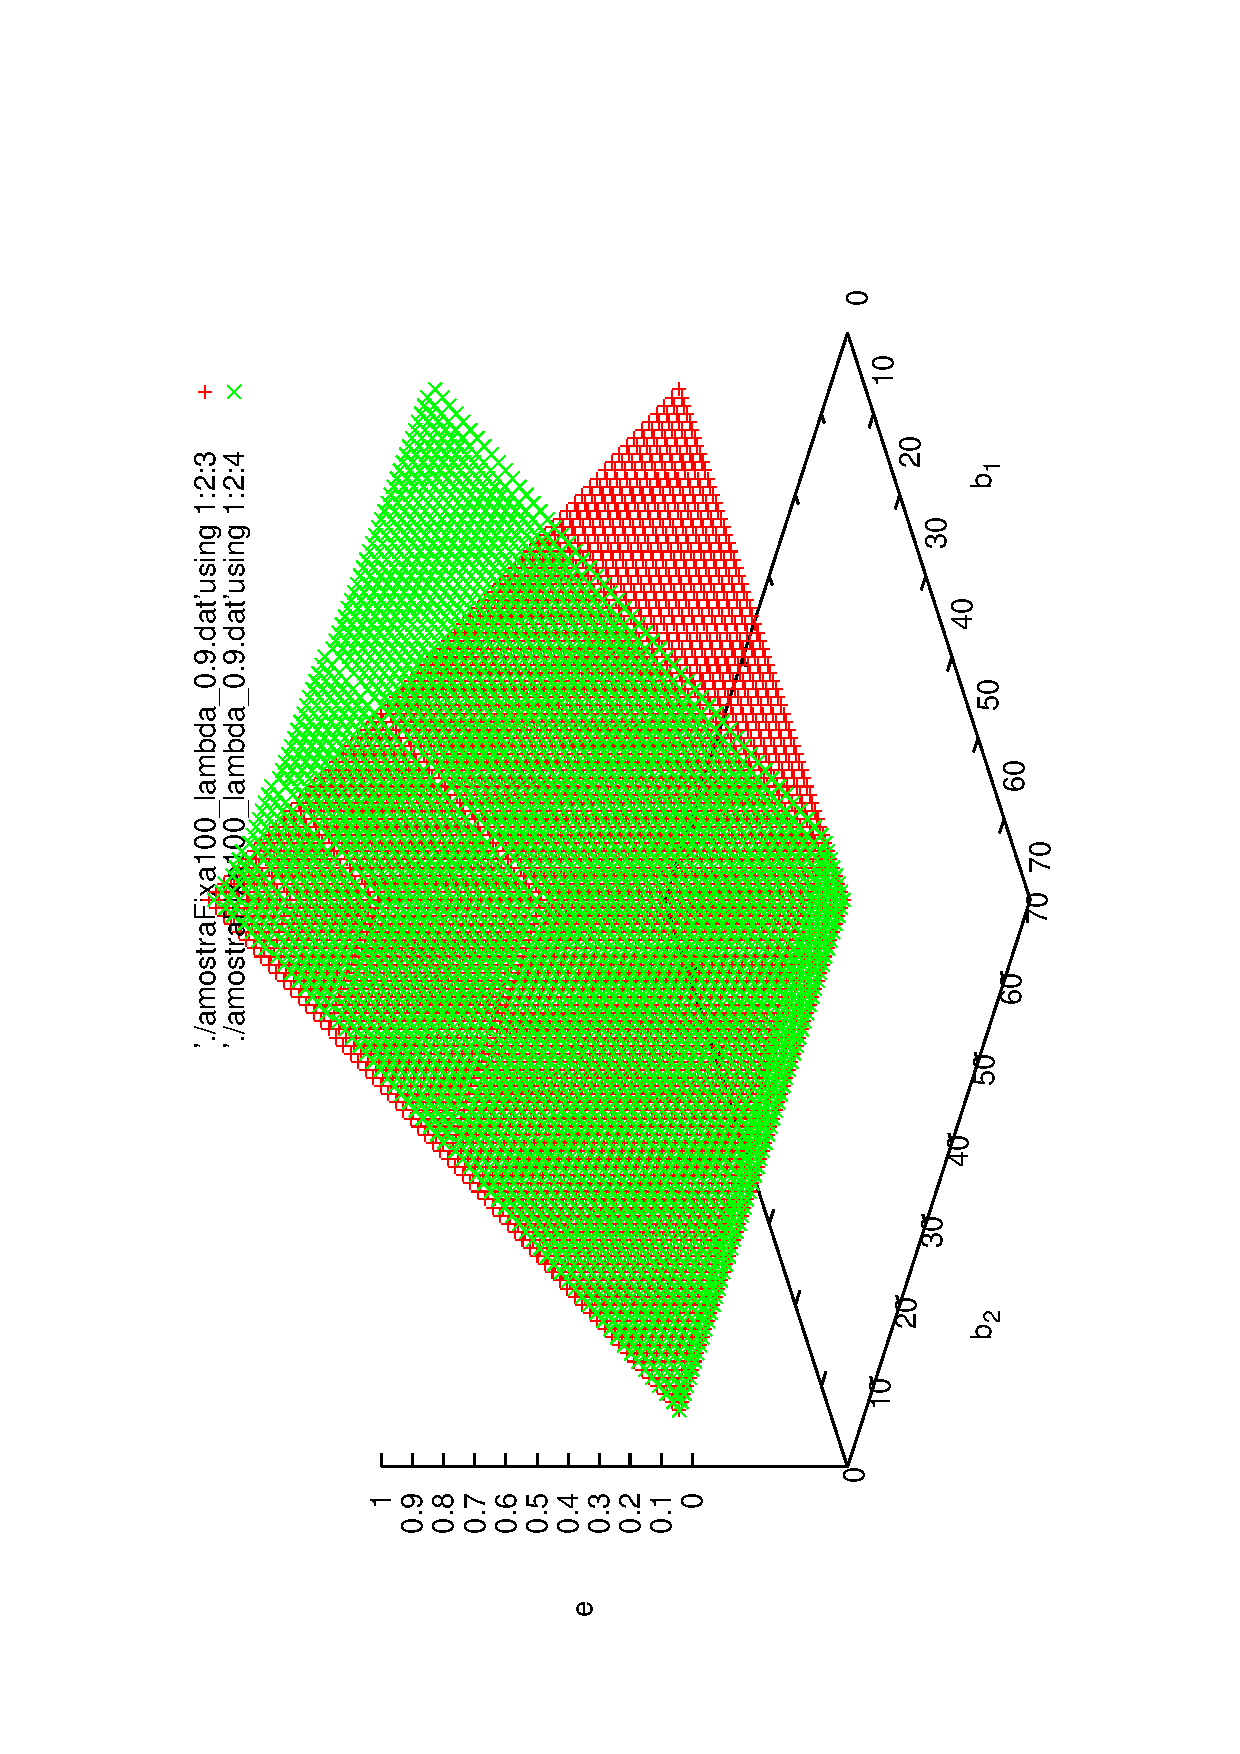
\includegraphics[scale=0.3,angle=-90]{fig24}
  \label{fig24}
  }\subfigure[Difference in efficiency of the methods I and II.]{
  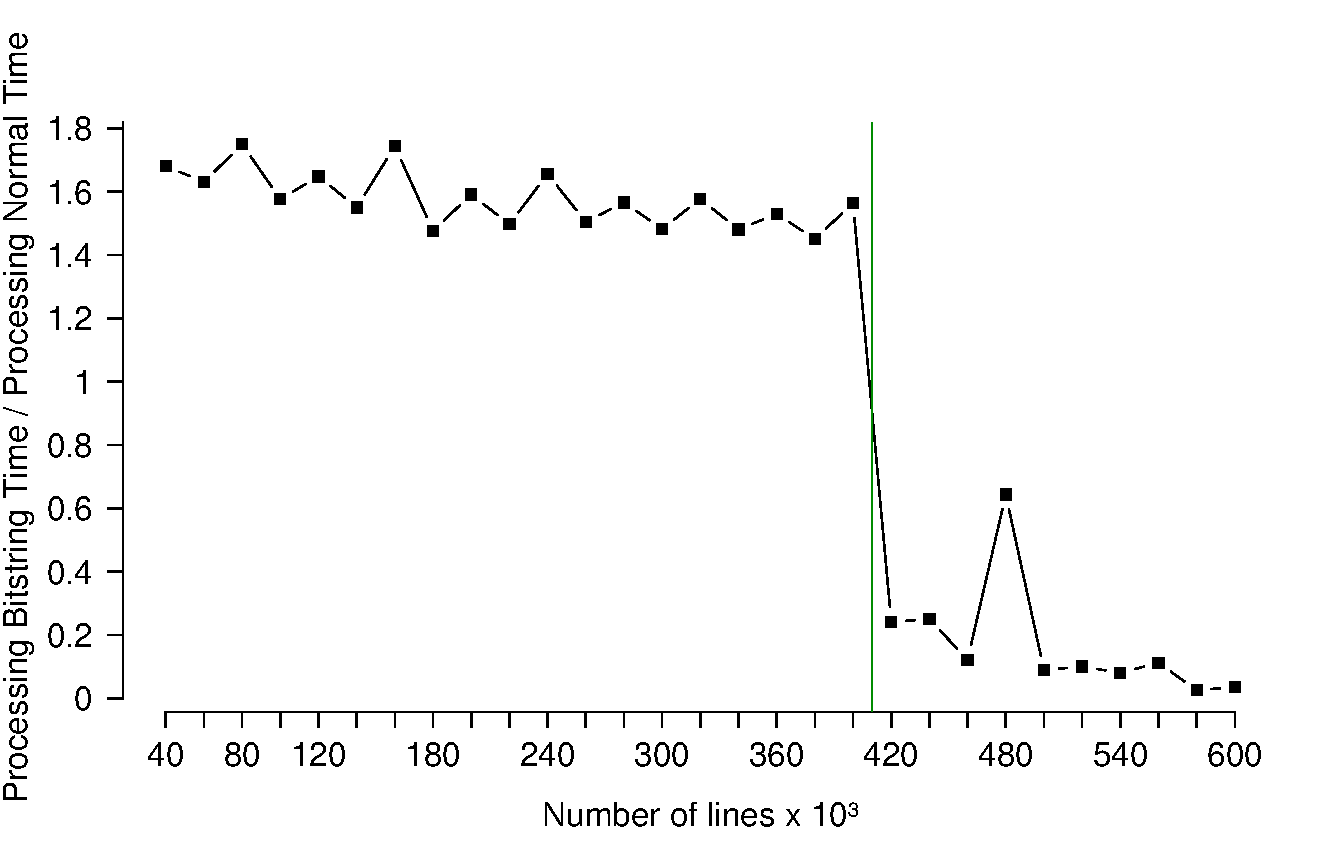
\includegraphics[scale=0.3,angle=-90]{fig25}
  \label{fig25}
  }
  \caption{Efficiency of the methods I and II in the data compression process of a matrix of numbers which require the same amount of bits to be represented.}
  \label{fig:2125}
\end{figure}

The two methods presented allow the storage and information manipulation in the compressed form, which provides an data managing large amounts optimization. The next step in the work development is the implementation of the proposed methods, as well as tests to be performed on data large volumes.

\section*{Discussion}

\subsection*{Which method to use?}

To know the best methodology to be applied to compress the data matrix, it becomes necessary to evaluate the numbers present in the matrix and as a consequence verify the bits number behavior needed to represent them. The first methodology provides greater efficiency when the bit number to store the information in the matrix are close. The second approach is to try to minimize losses when the numbers have outliers. For example, when it is desired to store values ​​of different magnitudes, such as 0, 1 and 1023. In this values range​​, it can be seen that the values ​​0 and 1 only need 1 bit, while the number 1,023 demand 10 bits. Following the first methodology, we would have to divide the strip into regions of 10 bits, which for storing the values ​​0 and 1, causes loss occurs 9 bits (Equation \ref{eq:19}), not allowing for more efficient compression. For work around this problem the second methodology can be applied, promoting data compression. In this case, instead of using 10 bits would be used 
only 5, with 1 bit to store the value and the other 4 to store the size of the region that this amount will be allocated (Equation \ref{eq:20}). See that the second method requires only 24 bits to represent the three values​​, unlike the first, which requires 30 bits.

\begin{equation} \label{eq:19}
 0000000000000000000000000000000000\underbrace{1111111111}_{1023}\underbrace{\overbrace{000000000}^{\text{Lost}}1}_{1}\underbrace{\overbrace{000000000}^{\text{Lost}}0}_{0}
\end{equation}

\begin{equation} \label{eq:20}
 0000000000000000000000000000000000000000\underbrace{1111111111}_{1023}\underbrace{1010}_{10}\underbrace{1}_{1}\underbrace{0001}_{1}\underbrace{0}_{0}\underbrace{0001}_{1}
\end{equation}

To verify the efficiency behavior ($\zeta$) compression process data, an analysis will be conducted on the bit number behavior used to store the information in a matrix with $r$ rows and $c$ columns. Consider the following equation \ref{eq:21}. This equation gives a percentage of the level of data compression.

\begin{equation} \label{eq:21}
 \zeta = \frac{\text{bits reserved } - \text{bits really needed}}{\text{bits reserved}}
\end{equation}

Consider a matrix $M_{r \times c}$, with $r$ rows and $c$ columns, we have in total $rc$ elements. To represent these elements in the worst case the, we have to reserve $64 \times rc$ bits. However, if these elements demanding only $b$ bits each represent, in total, would require $b \times rc$ bits. The function efficiency is presented in Equation \ref{eq:22}.

\begin{equation}\label{eq:22}
 \zeta = \frac{64 \times rc - b \times rc}{64 \times rc}
\end{equation}

Simplifying the Equation \ref{eq:22}, we obtain the equation \ref{eq:23}. The equation resulting from the simplification process does not depend on element number, but the bit number that is used.

\begin{equation} \label{eq:23}
 \zeta(b) = \frac{64  - b }{64}
\end{equation}

The equation \ref{eq:23} supplies in a direct way to efficiency in the worst and best case compression. In the worst case, $b = 64$, ie, at least one of the elements of the matrix M require 64 bits to be represented, resulting in $\zeta(64)=0\%$. As for the best case, $b=1$, the greater efficiency that can be achieved is $\zeta(1)=98.43\%$. For intermediate cases, it can be seen in Figure \ref{fig:01} efficiency behavior according to the bit number needed ($b$). This efficiency analysis  with respect to the first compression method presented in which all elements require the same bit number to be represented in memory.

\begin{figure}[h]
 \centering
 \psfrag{e}{$\xi$}
 \includegraphics[scale=0.5]{fig01}
 \caption{Compression efficiency behavior with respect to bit number.}
 \label{fig:01}
\end{figure}

For the second method, wherein the compression depends on the value to be stored, it should perform another analysis. This method considers that the elements demanding different bit number and this difference will determine the bit economy. We will analyze this configuration considering some numbers groups that can be represented by the same bit number as possible and when compared with the first method.

Again consider the matrix $M_{r \times c}$, only the $rc$ elements are divided into $g$ groups, where each group has $f_i$ numbers. For each element $b_i$ bits are reserved , corresponding to bits required to represent the desired number and $k$ bits, which represent the bit number to be reserved for storing the strip $b_i$ bits. The efficiency function has to be modified as shown in Equation \label{eq:24}.

\begin{equation}\label{eq:24}
 \zeta = \frac{64 \times rc - \sum_{i=1}^{g} ( b_i + k ) \times f_i }{64 \times rc} 
\end{equation}

Equations \ref{eq:25} to \ref{eq:27} are realized manipulations to adjust the equation. The equation that will provide the compression percentage  is apresented in Equation \ref{eq:30}.

\begin{equation} \label{eq:25}
 \zeta = \frac{64 \times rc - \sum_{i=1}^{g} ( b_i \times f_i + k \times f_i )}{64 \times rc} 
\end{equation}

\begin{equation} \label{eq:26}
 \zeta = \frac{64 \times rc - \sum_{i=1}^{g}  b_i \times f_i  -\sum_{i=1}^{g}  k \times f_i }{64 \times rc} 
\end{equation}

\begin{equation} \label{eq:27}
 \zeta = \frac{64 \times rc - \sum_{i=1}^{g}  b_i \times f_i  - k \times\sum_{i=1}^{g}  f_i }{64 \times rc} 
\end{equation}

\noindent as

\begin{equation} \label{eq:28}
 \sum_{i=1}^{g} f_i = rc
\end{equation}

\begin{equation} \label{eq:29}
 \zeta = \frac{64 \times rc - \sum_{i=1}^{g}  b_i \times f_i  - k \times rc }{64 \times rc} 
\end{equation}

\begin{equation}\label{eq:30}
 \zeta = 1 - \frac{\sum_{i=1}^{g}  b_i \times f_i }{64 \times rc} - \frac{k}{64} 
\end{equation}

\noindent whereupon

\begin{equation} \label{eq:31}
 k = \pi(\text{ greater value of }M_{r \times c})
\end{equation}

In a first example, we suppose again with the matrix M with $rc$ elements, such that the half of elements demanding demand 1 bits to represented and the other half 64 bits to be represented. So in this case i = 2, $b_1=1 $bits, $b_2=64$ bits and $f_i = \frac{rc}{2}$ for $i = 1 \text{ and } 2$. As the largest demand 64-bit value, then $k=7$, applying the Equation \ref{eq:31}. Efficiency in the bit economy can be calculated using Equation \ref{eq:30}, after performing the operations, equations \ref{eq:32} to \ref{eq:36}, we obtain the approximate value of $38.29\%$ for compression efficient.

\begin{equation} \label{eq:32}
 \zeta = 1 - \frac{\sum_{i=1}^{2}  b_i \times f_i }{64 \times rc} - \frac{7}{64} 
\end{equation}

\begin{equation} \label{eq:33}
 \zeta = 1 - \frac{  1 \times \frac{rc}{2} + 64 \times \frac{rc}{2} }{64 \times rc} - \frac{7}{64} 
\end{equation}

\begin{equation} \label{eq:34}
 \zeta = 1 - \frac{  32.5  \times rc }{64 \times rc} - \frac{7}{64} 
\end{equation}

\begin{equation} \label{eq:35}
 \zeta \approx 1 - 0.5078 - 0.1093
\end{equation}

\begin{equation} \label{eq:36}
 \zeta \approx 38.29\%
\end{equation}

See that the economy efficiency in using the second method was approximately 38\%. What is will influence the size of each number groups, which can be considered as the frequency with which these numbers appear. In the problem presented earlier, we considered two number groups, in which each group had half of elements to be compressed. Let's change the proportion of the groups, but now we use the classical definition of probability to assist in the analysis.

According to the definition the Laplace to the probability refers to the relationship between the case numbers and probable possible case numbers, for example, the relationship between the elements of a subset A,  probable case number, with the elements of set $\Omega$ , the possible case number, such that $A \in \Omega$. Thus, the probability of the subset A is defined as:

\begin{equation}
 P(A) = \frac{\text{Probable case numbers}}{\text{Possible case numbers}} = \frac{\text{Element number in A}}{\text{Element number in }\Omega}
\end{equation}

With this definition it is possible to associate the problem studied. The sample $\Omega$ space is formed by the elements of the matrix to be compacted. The subsets are formed by number groups in the array. Therefore, following this reasoning, we can rewrite the equation \ref{eq:30}, being defined in Equation \ref{eq:37}. In Equation \ref{eq:37}, the term $\frac{f_i}{rc}$ is replaced by $p_i$, and represents the probability of elements from group i forming the matrix M.

\begin{equation}\label{eq:37}
 \zeta = 1 - \frac{\sum_{i=1}^{g}  b_i \times p_i }{64} - \frac{k}{64} 
\end{equation}

\noindent with

\begin{equation}\label{eq:38}
 p_i = \frac{f_i}{rc}
\end{equation}

With the equation \ref{eq:37} can analyze the group proportion influence in the compression efficiency. Consider again the matrix M with $r$ rows and $c$ columns, totaling $rc$ elements. Now consider two groups of numbers whose ratio is defined by Equation \ref{eq:39}.

\begin{equation} \label{eq:39}
 p_1 + p_2= 1\text{, } p_1 \geq 0 \text{ and } p_2 \geq 0
\end{equation}

\noindent Thus, $p_1$ and $p_2$ define the number proportion of the matrix M requiring 1 bit and 64 bits to be represented, respectively. Thus, efficiency is defined in Equation \ref{eq:40}.

\begin{equation}\label{eq:40}
 \zeta = 1 - \frac{1 \times p_1  + 64 \times p_2}{64} - \frac{7}{64} 
\end{equation}

Now, we can verify what the proportions allowing a higher and lower compression from the equation \ref{eq:40}. If $\zeta=1$, then the efficiency is maximum and if $\zeta=0$, a efficiency is minimum. To calculate the values ​​of $p_1$ and $p_2$ so that efficiency is maximum, we must solve the system shown in Equation \ref{eq:41}. This system appears from the combination of equations \ref{eq:37}, with $\zeta=0$, with two number sets, one representing the elements represented by 1 bit and other  64-bit, with probability of $p_1$ and $p_2$, respectively with the equation \ref{eq:39}.

\begin{equation}\label{eq:41}
  \left
  \{\begin{matrix}
    p_1 + p_2 = 1\\ 
    p_1+64p_2 = 7
  \end{matrix}
  \right.
\end{equation}

Solving the system, we have that when $p_1=0.9047$ and $p_2=0.0953$ efficiency is maximum. Therefore, when approximately 90\% of the numbers require only one bit to be represented and approximately 10\% require 64 bits, the efficiency is maximum in this case equal to 87.5\%. Already in case the efficiency is minimal, we must solve the system shown in Equation \ref{eq:42}.

\begin{equation}\label{eq:42}
  \left
  \{\begin{matrix}
    p_1 + p_2 = 1\\ 
    p_1+64p_2 = 57
  \end{matrix}
  \right.
\end{equation}

Thus, when $p_1=0.1111$ and $p_2=0.8889$ is efficiency minimal according to the second method. For other combinations verify to Table \ref{tab:02}. Evaluating the table, you can verify two proportions negative when ($p_1$,$p_2$) assume the values ​​(0,1) and (0.1,0.9). It can be interpreted as the need to allocate more memory to use the method, since for the lower efficiency is reached, the value should be $p_1=0.9047$ e $p_2=0.0953$. In Table, we have an efficiency of 8\% ​​in the case of data compression, following the second proposed method, it should have in matrix 20\% of the elements represented with 1 bit and 80\% represented by 64 bits. If these proportions were maintained and the method was applied first, the efficiency would be minimal in all cases, because the greatest value is represented by 64 bits, which makes the division of the strip to store other values​​.

\begin{table}[h]
 \centering
 \caption{Combinations $p_1$ and $p_2$ to calculate the efficiency.}
 \begin{tabular}{ccc}
  \hline 
  $p_1$  & $p_2$ & Efficiency \\
  \hline
  0.0	&1.0    &-0.109 \\
  0.1	&0.9	&-0.010 \\
  0.2	&0.8	&0.087 \\
  0.3	&0.7	&0.185 \\
  0.4	&0.6	&0.284 \\
  0.5	&0.5	&0.382 \\
  0.6	&0.4	&0.481 \\
  0.7	&0.3	&0.579 \\ 
  0.8	&0.2	&0.678 \\
  0.9	&0.1	&0.776 \\ 
  1.0	&0.0	&0.875 \\
  \hline
 \end{tabular}
 \label{tab:02}
\end{table}

Until the moment, we used only two number groups, just a question being examined is how different combinations of these numbers may influence the effectiveness of the compaction process by using two proposed methods.

As an example, we calculated the efficiency for different number groups with the same element number, or rather the same frequency. Note below the efficiencies calculated:

\begin{itemize}
  \item 3 number groups that require numbers 1, 32 and 64 bits, efficiency $\zeta=0.3854$,
  \item 5 number groups that require numbers 1, 16, 32, 48 and 64 bits, efficiency $\zeta=0.3875$,
  \item 8 number groups that require numbers 1, 8, 16, 24, 32, 40, 48, 56 and 64 bits, efficiency $\zeta=0.3888$
\end{itemize}

When groups are proportionality, ie, have the same frequency, as consequence the same probability of occur, the efficiency is almost the same, using the second method apresented.

Leveraging the idea frequency, which may be generalized as the probability that a number sets can occur, we use probability distributions, in this case the discrete to determine the element numbers in each groupie the frequency. With this, it becomes possible to evaluate, even in an approximate way the proposed methods efficiency behavior. In the case presented earlier, it can be seen that the distribution was uniform discrete was used to determine the bits number, since the probability of occurrence of each group was the same.

To illustrate the calculation, we use three probability distributions: Discrete Uniform, Binomial and Poisson. It is considered that the bit numbers of the numbers to be allocated to matrix follow these three distributions. The respective parameters, thus, relate to the bit number in the uniform discrete case $U(a=1,b=64)$, which states that the number probability is represented by 1, 2, 3, $\ldots$, 64 is the same, ie, $\frac{1}{64}$. In the binomial case, it is considered that $B(n,0.5)$, such that the success numbers n represents the maximum bit number to represent the matrix numbers being equal to 1, 8, 16, 32 and 64, with a probability equal to 0.5 assuming a bit value 0 or 1. In the Poisson distribution, the parameter Poisson ($\lambda=p$) being the bit numbers expected to represent the element matrix. For all the simulations, it is considered that $k=7$, that is, it is considered that there is a possibility of occur a number that requires 64 bits.

Thus, the efficiency is calculated to be as small as possible, because if the value of k decreases, efficiency increases, as can be seen in Equation \ref{eq:37}.

To analyze about this new viewpoint, consider a sample of $rc$ elements, corresponding to the matrix element number $M_{r \times c}$. Therefore, a sample generating $rc$ elements can completely fill the matrix and verify the efficiency of the compression method proposed.

Consider that the numbers composing the matrix suggested requiring a bit numbers which follow a discrete uniform distribution $U(a=1,b=64)$. To verify the efficiency, generates a sample with 100 ($M_{10 \times 10}$), 10,000 ($M_{100 \times 100}$) and 1,000,000 ($M_{1,000 \times 1.000}$) numbers . Since this is a simulation, are generated 1,000 samples, for each calculated efficiency and the computed final average. The results can be seen in Table \ref{tab:03}. If the numbers follow the distribution, the efficiency of the proposed method is approximately 40\%.

\begin{table}[h]
  \centering
  \caption{Results of the simulation process efficiency on matrices whose elements are the bits number determined by a Discrete Uniform distribution $U(a=1,b=64)$.}
 \begin{tabular}{cc}
    \hline
    Sample size& Efficiency \\
    \hline
     100	& 0.3760938 \\
     1,000 	& 0.3795953 \\
     10,000 	& 0.3826869 \\
    \hline
 \end{tabular}
 \label{tab:03}
\end{table}

We analyzed the performance another simulation, only now the bit number follows a binomial distribution $B(n,0.5) $, such that the successes number n represents the maximum bit number to represent the matrix numbers being equal 1, 8, 16, 32 and 64, with a probability equal to 0.5 assuming a bit value 0 or 1. In this case, we analyze the efficiency behavior as a function of the parameter $n$, the bit number required, in efficiency of data compression. Results can be seen in Table \ref{tab:04}. Note that when smaller the bit number to represent array elements, the efficiency level is high using the second method. However, for the case in which the elements require 64 bits, the efficiency is negative. This result indicates that using the second method, when elements require 64 bit this becomes impractical, because it would be require more memory to allocate the compressed matrix.

\begin{table}[h]
  \centering
  \caption{Results of the simulation process efficiency on matrices whose elements are the bit number determined by a binomial distribution $B(n,0.5)$, such that the successes number n represents the maximum bit number to represent the matrix numbers being equal to 1, 8, 16, 32 and 64, with a probability equal to 0.5 assuming a bit value 0 or 1.}
 \begin{tabular}{cccc}
    \hline
			& 		&Efficiency         & \\
    \hline
			&  		&Sample size & \\
    Strip size		& 100		& 1,000		    & 1,000,000 \\
    \hline
     1 			&  0.9760937	& 0.9764797 	    & 0.9765566 \\
     8			&  0.8109375	& 0.8128453 	    & 0.8125079 \\
     16			&  0.626875	& 0.6251859 	    & 0.6249333 \\
     32			&  0.2476562	& 0.2504953 	    & 0.2499712 \\
     64			&  -0.5004688	& -0.4999828 	    & -0.5000366 \\
    \hline
 \end{tabular}
 \label{tab:04}
\end{table}

It is now considered that the bit number distribution is described by a Poisson ($\lambda$). Now the parameter $\lambda$ can be considered as the expected bit number  to represent numbers in matrix. Values ​​greater than 64 generated in this simulation were considered as being equal to 64. The results for this simulation can be seen in Table \ref{tab:05}. Note that increasing the bit number to represent numbers increases, there is a loss of efficiency in the compression process. Another interesting fact is the emergence of a negative efficiency. In this case, for values ​​generated with a $\lambda=64$, the second method requires more memory to allocate the matrix formed by elements generated from this distribution.

\begin{table}[h]
  \centering
  \caption{Results of the simulation process efficiency on matrices whose elements are the bit number determined by a Poisson distribution ($\lambda$), such that $\lambda$ represents the bit number to represent the expected matrix numbers.}
 \begin{tabular}{cccc}
    \hline
			& 	&Efficiency         & \\
    \hline
			&  	&Size sample& \\
    $\lambda$		& 100	& 1,000		    & 1,000,000 \\
    \hline
     1	& 0.8746875 & 0.8749859   & 0.8749834 \\
     8 	& 0.7657812 & 0.7656016   & 0.7656138 \\
     16	& 0.6300000 & 0.6400594   & 0.6405952 \\
     32	& 0.3851562 & 0.3903531   & 0.3903477 \\
     64	& -0.0528125& -0.05984375 & -0.05953145 \\
    \hline
 \end{tabular}
 \label{tab:05}
\end{table}

As the bits amount that form the numbers composing the matrix M are considered random variables, we can perform an analysis of the expected values ​​and the variability of the data to verify the compression efficiency level.

Consider that the bit number (B) to represent the M matrix elements are defined as a random variable, $B \sim U(a=1,b=64)$, then applying the expected value in the equation \ref{eq:43}, we have

\begin{equation}\label{eq:43}
 E(\zeta) = 1 - \frac{\sum_{i=1}^{g}  b_i \times p_i }{64} - \frac{k}{64} 
\end{equation}

\noindent as $E(b_i) = \sum_{i} b_i \times p(b_i) = \frac{a+b}{2}$, it result in 

\begin{equation}\label{eq:44}
 E(\zeta) = 1 - \frac{E(B)}{64} - \frac{k}{64} 
\end{equation}

Recovered the example used, consider that there are two groups, $b_1=1$ and $b_{64}=64$, implying that $k=7$. Since $E(X)=\frac{a + b}{2}$, when $X \sim U(a,b)$, the efficiency is defined in Equation \ref{eq:45}.

\begin{equation}\label{eq:45}
 E(\zeta) = 1 - \frac{\frac{1+64}{2}}{64} - \frac{7}{64} \approx 38.29\% 
\end{equation}

This result corroborates with the findings anteriorly found in Table \ref{tab:03}. The same principle can be applied when the bit number (B) is a random variable with Binomial and Poisson distributions already displayed. In the case of Binomial when $B \sim B(n=64,p)$, has

\begin{equation}\label{eq:46}
 E(\zeta) = 1 - \frac{\sum_{i=1}^{g}  b_i \times p_i }{64} - \frac{k}{64} 
\end{equation}

\noindent in this case $E(b_i) = \sum_{i} b_i \times p(b_i) = n \times p$

\begin{equation}\label{eq:47}
 E(\zeta) = 1 - \frac{64 \times p }{64} - \frac{k}{64} 
\end{equation}

Again, it is considered that $n=64$ and $p=0.5$ as the success probability of occurring a number that requires 64 bits to be represented, then $k=7$. As a result we obtain

\begin{equation}\label{eq:48}
 E(\zeta) = 1 - \frac{64 \times 0.5 }{64} - \frac{7}{64} \approx 39.05\%
\end{equation}

The value found can be seen in Table \ref{tab:04}, obtained through simulations. As for the Poisson case, the efficiency value is defined as

\begin{equation}\label{eq:49}
 E(\zeta) = 1 - \frac{\sum_{i=1}^{g}  b_i \times p_i }{64} - \frac{k}{64} 
\end{equation}

\noindent in this case $E(b_i) = \lambda$,

\begin{equation}\label{eq:50}
 E(\zeta) = 1 - \frac{\lambda}{64} - \frac{k}{64} 
\end{equation}

We consider $\lambda = 1$, 

\begin{equation}\label{eq:51}
 E(\zeta) = 1 - \frac{\lambda}{64} - \frac{k}{64}  = 1 - \frac{1}{64} - \frac{7}{64} \approx 87.5\%
\end{equation}

The efficiency level calculated $\zeta \approx 87.5\%$ can be seen in Table \ref{tab:05}. The results presented show simulations and verify that the compression process occurs in different cases.

In all tests so far conducted, we analyzed the impact of the average data compression efficiency. The final analysis to be performed, consider the mean and variance of the numbers to be compressed. Thus, it is expected function and efficiency in calculating the mean and variance of matrix numbers. (Remover?)

% You may title this section "Methods" or "Models". 
% "Models" is not a valid title for PLoS ONE authors. However, PLoS ONE
% authors may use "Analysis" 
\section*{Materials and Methods}

\section{Matrix compression}

The matrix compression process consists in reducing the bytes number required to allocate a matrix in memory. This process allows a greater amount of information to be stored using the same hardware available memory allocation traditional method. One of the advantages in applying this method is the possibility to work with large information amounts about data directly from memory without need for disk access, reading and writing, which burdens the processing.

The steps and implementations required to use the prepossessing method are described below. Consider a matrix $M_{r \times c}$ in which $r$ is the rows number and $c$ the columns number. Each element of this matrix, called $m_{ij}$, only stores an integer number. For an integer number being stored in the memory of a 64-bit processor, using the largest number of available bits, demand is 64 bits. Therefore, the bit number ($\Delta$) required to allocate all the elements of a matrix M in the traditional manner may be defined by:

\begin{equation}\label{eq:01}
  \Delta = l \times c \times 64
\end{equation}

The $\Delta$ represents a greater bit number than that actually used. Assume that in a matrix, for example, there are only elements with values ​​equal to 0 or 1. These values ​​are represented in binary by only one bit. Therefore, when one is allocated in variable that requires 64 bits to be stored in memory, there is a loss of 63 bits, which could be used to store other numbers or information. This example deals with the case more expressive with respect to waste memory. The bit number calculation $\delta$ really necessary to implement this example is represented in the Equation \ref{eq:02}.

\begin{equation}\label{eq:02}
  \delta = l \times c \times 1
\end{equation}

The bits economy $\xi$ can be represented by the difference between $\Delta$ and $\delta$ (Equations \ref{eq:03} to \ref{eq:06}).

\begin{equation}\label{eq:03}
 \xi = \Delta - \delta
\end{equation}

\begin{equation}\label{eq:04}
 \xi =  r \times c \times 64 - r \times c \times 1
\end{equation}

\begin{equation}\label{eq:05}
 \xi =  r \times c \times (64 -  1)
\end{equation}

\begin{equation} \label{eq:06}
 \xi =  r \times c \times 63
\end{equation}

Based on the Equations \ref{eq:01} to \ref{eq:06}, it is can to observe that the economy $\xi$ is high, because $r \times c$ elements require only $r \times c \times  1$ bits instead of $r \times c \times 64$ bits. The same happens with other values ​​that do not need 64 bits to be represented in memory, because it not always all bits are used. It can be said that the economy grows linearly with the number of array elements.

There are two ways to perform the manipulations of these bits to minimize wasted space. Each of these forms follows a specific methodology to be applied to certain cases. 

\subsection*{The first method: Analyzing the greatest value to allocate in a matrix}

The first methodology consists in determining the value of the largest element $\theta$, which should be stored in the matrix and as a result determines the  largest bit number ($\pi$) really need to store that value. The bit number ($\pi$) can be directly approximated by the equation \ref{eq:07}. This approach consists in calculating the bit value needed to represent the value, as there is usually decimal, the value 1 which is added ensures, that the resulting bit number to be correct to store such value, the integer part of the operation.

\begin{equation} \label{eq:07}
 \pi(\theta) \approx \begin{cases}
	1, &  \text{ if } \theta = 0 \\ 
	\left( \frac{log(\theta)}{log(2)}  \right) + 1,  & \text{ if } \theta > 0  
	\end{cases}
\end{equation}

Each matrix element of M, denoted by $m_{ij}$, is represented by a strip composed of 64 bits. In the example mentioned, for values ​​0 and 1, the value of $\theta$ equals 1, ie, in a strip of 64 bits may be allocated 64 values. Each bit of this strip will represent one of the values ​​to be allocated. This fact is responsible for saving bits, for 64 values​​, which were traditionally stored in $r \times c \times 64$  bits are stored in only $r \times c$ bits.

Suppose that the greatest value to be stored in a matrix $\Phi$ is $\theta=1023$. Therefore, the bit number required to represent that really value is $\pi=10$, because the number 1023 in binary base is 1111111111, therefore, demand 10 bit and the other 54 bits zeros disregarding the right, to be represented in memory. Consider a matrix $\Phi$ represented in equation \ref{eq:08}.

\begin{equation} \label{eq:08}
  \Phi = \begin{bmatrix}
  900 & 1023 & 721 & 256 & 1 & 10 & 700 & 20 & \hdots\\ 
  \vdots & \vdots & \vdots & \vdots & \vdots & \vdots & \vdots & \vdots & \ddots 
  \end{bmatrix}
\end{equation}

The values ​​of the matrix $\Phi$ in binary are represented in Table \ref{tab:01}. It is possible
checking the bit number necessary to represent the values​​, then it can be concluded
that with 10 bits, it is can represent all numbers.

\begin{table}[h]
 \centering
 \caption{Some matrix elements $\Phi$ represented in binary base. It is can to verify that using 10 bits is possible to represent the all values.}
 \begin{tabular}{cccc} 
  \hline 
  Element & Value  & Binary & Bit number necessary\\
  \hline
  $\Phi_{1,1}$ & 900  & 1110000100 & 10\\
  $\Phi_{1,2}$ & 1023 & 1111111111 & 10\\
  $\Phi_{1,3}$ & 721  & 1011010001 & 10\\
  $\Phi_{1,4}$ & 256  & 100000000  & 9\\
  $\Phi_{1,5}$ & 1    & 1          & 1\\
  $\Phi_{1,6}$ & 10   & 1010       & 4\\
  $\Phi_{1,7}$ & 700  & 1010111100 & 10\\
  $\Phi_{1,8}$ & 20   & 10100      & 5\\
  \hline
 \end{tabular}
 \label{tab:01}
\end{table}

Consider a matrix $\phi$, such that the matrix will store the the matrix $\Phi$ values, only using the bit number actually required so that there is not wastage. According to this methodology, the first element of the matrix $\phi$, denoted by $\phi_{1,1}$, which has a strip of 64 bits associated, it will be partitioned into regions. Each of these regions will store the values ​​of the matrix $\Phi$. As it takes 10 bits to represent the values ​​of the matrix $\Phi$, the bit element strip $\phi_{1,1}$ will contain 6 regions, such that each region will bundle 10 bits. So overall, this strip will have 6 regions, totaling 60 bits. The 4 bits free remaining it would be used later. The elements bit strip of $\phi_{1,1}$ can be verified in the equation \ref{eq:09}. It is possible to observe the regions, the values ​​stored (binary and decimal), and the bits that are left initially.

\begin{equation}\label{eq:09}
 \phi_{1,1} = 0000\underbrace{0000001010}_{10}\underbrace{0000000001}_{1}\underbrace{0100000000}_{256}\underbrace{1011010001}_{721}\underbrace{1111111111}_{1023}\underbrace{1110000100}_{900} 
\end{equation}

The process of allocation values ​​is performed as follows: the element $\Phi_{1,1}=900$ is stored in the first region of the element strip $\phi_{1,1} $, which corresponds to bits 0 to 9. Already for the element $\Phi_{1,2}=1,023$ is allocated in the second region, from 10 to 19 bits and the same with the other elements. Thus, the elements $\Phi_{1,i}$, with $i=1,\ldots,7$ are stored on the strip element $\phi_{1,1}$. Already the seventh element, $\Phi_{1,7}=700$, should be divided into two parts, so that a part are stored in the strip element $\phi_{1,1}$ and the other in the element strip $\phi_{1,2}$. The process of division shown in equation \ref{eq:10}, it can be seen the place where the split occurs strip element $\Phi_{1,7}=$ 700 in the parts $a$ and $b$. In the equation \ref{eq:11}, it can verify the bits grouped, demonstrating that it is possible to recover the information.

\begin{equation}\label{eq:10}
  \underbrace{\underbrace{0000010100}_{20}\overbrace{101011}^{a}}_{\phi_{1,2}}|\underbrace{\overbrace{1100}^{b}\underbrace{0000001010}_{10}\underbrace{0000000001}_{1}\hdots}_{\phi_{1,1}}
\end{equation}

\begin{equation}\label{eq:11}
  \underbrace{0000010100}_{20}\underbrace{\overbrace{101011}^a|\overbrace{1100}^{b}}_{700}\underbrace{0000001010}_{10}\ldots
\end{equation}

In a general way, what happens is the storage of the matrix elements $\Phi$ in a matrix $\phi$, such that the bits required to store them in the array $\phi$ is much smaller than the matrix $\Phi$, due to reorganization of the data. Even with the compression of the data, the information can be retrieved, thus justifying the proposed procedure.

\subsection*{The second method: Analyzing the values ​​that will be allocated in a matrix}

A second proposed method tries to make a new form of data compression. Consider again the matrix described in Equation \ref{eq:08}. Suppose the largest value stored in it is number 1023. As already demonstrated, to store this value in binary are necessary 10 bits. Now instead of reserving a region on the strip to store each value, reserves two regions. Such regions, one is used to store the bit number needed to represent the value and the second region will store the respective value. The first region will have a fixed size, in the example cited, 4 bits. The 4 bits are required to store the bit number necessary to store the largest value, in this case 10 bits. The size of the second region is determined by the value stored in the first. And so the other values ​​are stored.

To illustrate this methodology, we will be using the matrix represented in Equation \ref{eq:08}, called $\Phi$. The largest element of $\Phi$ is 1,023, as soon as the bit number required to represent this value is $\pi=10$ bits. The element $\Phi_{1,1}=900$ is stored in bits of the element strip of $\phi_ {1,1}$. To store the element $\Phi_{1,1}$, it should create the two first regions of the strip element $\phi_{1,1} $. Initially element strip $\phi_{1,1}=0$ is shown in equation \ref{eq:12}.

\begin{equation} \label{eq:12}
 \phi_{1,1} = 0000000000000000000000000000000000000000000000000000000000000000
\end{equation}

The first region that will store the value 10, because to represent the number 900 are need 10 bits. Then, it will have 4 bits, because represent the value 10, it demand 4 bits. The 4 bits are manipulated of according to the bit number to represent the largest value of $\Phi$, in which case, the value is 1,023. The strip $\phi_{1,1}$, after storing the information of $\Phi_{1,1}$ is shown in Equation \ref{eq:13}

\begin{equation} \label{eq:13}
 \phi_{1,1} = 00000000000000000000000000000000000000000000000000\underbrace{\underbrace{1110000100}_{\text{value} = 900}\underbrace{1010}_{\text{10 bits}}}_{900}
\end{equation}

Adding the elements $\Phi_{1,2}=1023$ and $\Phi_{1,3}=721$, the strip of $\phi_{1,1}$ updated is represented in Equation \ref{eq:14}. You can check the regions that store the information from the elements.

\begin{equation} \label{eq:14}
 \phi_{1,1} = 
 0000000000000000000000\underbrace{1011010001}_{721}\underbrace{1010}_{10}\underbrace{1111111111}_{1023}\underbrace{1010}_{10}\underbrace{1110000100}_{900}\underbrace{1010}_{10}
\end{equation}

Until this moment, the second method is using more bits to store a value that the first methodology. With the insertion of the fourth element that the bit economy occurs, because $\Phi_{1,4}=256$ demand only 9 bits. The first region with 4 bits defines how many bits the second region will contain the stored value. So instead of storing $\Phi_{1,4}=10$ in 10 bits, as in the previous method, it demands 9 bits, but it takes a whole 13 bits. The economy becomes evident when the element $\Phi_{1,5}=1$ is stored. Note that this element requires only 1 bit to be stored, so instead of 10 bits, only 1 bit is used, more 4 bits to indicate that the value is stored in only 1 bit. Therefore, instead of the 10 bits required to store that value pair following the first methodology, now only 5 bits are needed. The strip of $\phi_{1,1}$, after insertion of the latter two values ​​are updated in Equation \ref{eq:15}.

\begin{equation} \label{eq:15}
 \phi_{1,1} =
 0000\underbrace{1}_{1}\underbrace{0001}_{1}\underbrace{100000000}_{256}\underbrace{1001}_{9}\underbrace{1011010001}_{721}\underbrace{1010}_{10}\underbrace{1111111111}_{1023}\underbrace{1010}_{10}\underbrace{1110000100}_{900}\underbrace{1010}_{10}
\end{equation}

Now the element $\Phi_{1,6}=10$ will be inserted in the strip $\phi_{1,1}$. The process need that 4 bits are used element strip $\phi_{1,1}$ and another 4 bits of the element $\phi_{1,2}$. The strips updated element $\phi_{1,1}$ and $\phi_{1,2}$ can be verify in Equations \ref{eq:16} and \ref{eq:17}.

\begin{equation} \label{eq:16}
 \phi_{1,1} =
 \underbrace{0100}_{4}\underbrace{1}_{1}\underbrace{0001}_{1}\underbrace{100000000}_{256}\underbrace{1001}_{9}\underbrace{1011010001}_{721}\underbrace{1010}_{10}\underbrace{1111111111}_{1023}\underbrace{1010}_{10}\underbrace{1110000100}_{900}\underbrace{1010}_{10}
\end{equation}

\begin{equation} \label{eq:17}
 \phi_{1,2} = 000000000000000000000000000000000000000000000000000000000000\underbrace{1010}_{10}
\end{equation}

Adding the last two elements $\Phi_{1,7}=700$ and $\Phi_{1,8}=20$ in the element strip $\phi_{1,2}$, which after being updated, it can be viewed at equation \ref{eq:18}.

\begin{equation} \label{eq:18}
 \phi_{1,2} = 00000000000000000000000000000000000\underbrace{10100}_{20}\underbrace{0101}_{5}\underbrace{1010111100}_{700}\underbrace{1010}_{10}\underbrace{1010}_{10}
\end{equation}

For storing the elements of matrix $\Phi$ in the matrix $\phi$ were used 87 bits instead of 80 bits used in the first method. The choice of which method to use will be discussed in the section Discussion. The proposed methods have different levels of compression, depending directly from the values ​​that must be stored.

% Do NOT remove this, even if you are not including acknowledgments
\section*{Acknowledgments}


%\section*{References}
% The bibtex filename
\bibliography{plos.bib}

\section*{Figure Legends}
%\begin{figure}[!ht]
%\begin{center}
%%\includegraphics[width=4in]{figure_name.2.eps}
%\end{center}
%\caption{
%{\bf Bold the first sentence.}  Rest of figure 2  caption.  Caption 
%should be left justified, as specified by the options to the caption 
%package.
%}
%\label{Figure_label}
%\end{figure}


\section*{Tables}
%\begin{table}[!ht]
%\caption{
%\bf{Table title}}
%\begin{tabular}{|c|c|c|}
%table information
%\end{tabular}
%\begin{flushleft}Table caption
%\end{flushleft}
%\label{tab:label}
% \end{table}

\end{document}

